\documentclass[twoside]{book}

% Packages required by doxygen
\usepackage{calc}
\usepackage{doxygen}
\usepackage{graphicx}
\usepackage[utf8]{inputenc}
\usepackage{makeidx}
\usepackage{multicol}
\usepackage{multirow}
\usepackage{textcomp}
\usepackage[table]{xcolor}

% Font selection
\usepackage[T1]{fontenc}
\usepackage{mathptmx}
\usepackage[scaled=.90]{helvet}
\usepackage{courier}
\usepackage{amssymb}
\usepackage{sectsty}
\renewcommand{\familydefault}{\sfdefault}
\allsectionsfont{%
  \fontseries{bc}\selectfont%
  \color{darkgray}%
}
\renewcommand{\DoxyLabelFont}{%
  \fontseries{bc}\selectfont%
  \color{darkgray}%
}

% Page & text layout
\usepackage{geometry}
\geometry{%
  a4paper,%
  top=2.5cm,%
  bottom=2.5cm,%
  left=2.5cm,%
  right=2.5cm%
}
\tolerance=750
\hfuzz=15pt
\hbadness=750
\setlength{\emergencystretch}{15pt}
\setlength{\parindent}{0cm}
\setlength{\parskip}{0.2cm}
\makeatletter
\renewcommand{\paragraph}{%
  \@startsection{paragraph}{4}{0ex}{-1.0ex}{1.0ex}{%
    \normalfont\normalsize\bfseries\SS@parafont%
  }%
}
\renewcommand{\subparagraph}{%
  \@startsection{subparagraph}{5}{0ex}{-1.0ex}{1.0ex}{%
    \normalfont\normalsize\bfseries\SS@subparafont%
  }%
}
\makeatother

% Headers & footers
\usepackage{fancyhdr}
\pagestyle{fancyplain}
\fancyhead[LE]{\fancyplain{}{\bfseries\thepage}}
\fancyhead[CE]{\fancyplain{}{}}
\fancyhead[RE]{\fancyplain{}{\bfseries\leftmark}}
\fancyhead[LO]{\fancyplain{}{\bfseries\rightmark}}
\fancyhead[CO]{\fancyplain{}{}}
\fancyhead[RO]{\fancyplain{}{\bfseries\thepage}}
\fancyfoot[LE]{\fancyplain{}{}}
\fancyfoot[CE]{\fancyplain{}{}}
\fancyfoot[RE]{\fancyplain{}{\bfseries\scriptsize Generated on Tue Sep 9 2014 17\-:30\-:58 for D\-O\-S extraction by Doxygen }}
\fancyfoot[LO]{\fancyplain{}{\bfseries\scriptsize Generated on Tue Sep 9 2014 17\-:30\-:58 for D\-O\-S extraction by Doxygen }}
\fancyfoot[CO]{\fancyplain{}{}}
\fancyfoot[RO]{\fancyplain{}{}}
\renewcommand{\footrulewidth}{0.4pt}
\renewcommand{\chaptermark}[1]{%
  \markboth{#1}{}%
}
\renewcommand{\sectionmark}[1]{%
  \markright{\thesection\ #1}%
}

% Indices & bibliography
\usepackage{natbib}
\usepackage[titles]{tocloft}
\setcounter{tocdepth}{3}
\setcounter{secnumdepth}{5}
\makeindex

% Hyperlinks (required, but should be loaded last)
\usepackage{ifpdf}
\ifpdf
  \usepackage[pdftex,pagebackref=true]{hyperref}
\else
  \usepackage[ps2pdf,pagebackref=true]{hyperref}
\fi
\hypersetup{%
  colorlinks=true,%
  linkcolor=blue,%
  citecolor=blue,%
  unicode%
}

% Custom commands
\newcommand{\clearemptydoublepage}{%
  \newpage{\pagestyle{empty}\cleardoublepage}%
}


%===== C O N T E N T S =====

\begin{document}

% Titlepage & ToC
\hypersetup{pageanchor=false}
\pagenumbering{roman}
\begin{titlepage}
\vspace*{7cm}
\begin{center}%
{\Large D\-O\-S extraction }\\
\vspace*{1cm}
{\large Generated by Doxygen 1.8.6}\\
\vspace*{0.5cm}
{\small Tue Sep 9 2014 17:30:58}\\
\end{center}
\end{titlepage}
\clearemptydoublepage
\tableofcontents
\clearemptydoublepage
\pagenumbering{arabic}
\hypersetup{pageanchor=true}

%--- Begin generated contents ---
\chapter{Index}
\label{index}\hypertarget{index}{}\hypertarget{index_intro}{}\section{Introduction}\label{index_intro}
This program allows to extract the Density of States (Do\-S), assessed by means of capacitance-\/voltage measurements, in an organic semiconductor device. Simulated values are fitted to experimental data. \par
Source and header files are written in C++11 language. \par
The software is intended to be used on a Unix-\/like operating system.\hypertarget{index_dependancies}{}\section{Dependancies}\label{index_dependancies}
The program requires the following software to be installed on your system\-:

\begin{DoxyItemize}
\item \href{http://www.cmake.org}{\tt C\-Make} (version 2.\-8 or above), a cross-\/platform configuration tool; \item \href{http://www.gnu.org/software/make}{\tt Make} (version 3.\-8.\-1 or above), a utility to build executables; \item \label{index_GCC}%
\hypertarget{index_GCC}{}%
\href{http://www.gnu.org/software/gcc}{\tt G\-C\-C} (version 4.\-8 or above), the G\-N\-U Compiler Collection; \par
 \par
\item \label{index_Eigen}%
\hypertarget{index_Eigen}{}%
\href{http://eigen.tuxfamily.org}{\tt Eigen} (version 3.\-2 or above), to handle with matrices, vectors and linear algebra; \item \label{index_Gnuplot}%
\hypertarget{index_Gnuplot}{}%
\href{http://www.gnuplot.info}{\tt Gnuplot} (version 4.\-6.\-4 or above), a graphical utility to generate plots (the package {\bfseries gnuplot-\/x11}, a terminal for X servers, is also required for the interactive interface); \item \href{http://www.boost.org}{\tt Boost} (version 1.\-50 or above), a set of libraries used by \hyperlink{index_gnuplot-iostream}{gnuplot-\/iostream}; \item \label{index_Doxygen}%
\hypertarget{index_Doxygen}{}%
\href{http://www.doxygen.org}{\tt Doxygen} (version 1.\-8.\-6 or above), a documentation generator (not compulsory).\end{DoxyItemize}
It also uses the following libraries, shipped in the {\itshape include/} folder\-:

\begin{DoxyItemize}
\item \href{http://getpot.sourceforge.net}{\tt Get\-Pot} (version 1.\-1.\-18), to parse command-\/line and configuration files; \item \label{index_gnuplot-iostream}%
\hypertarget{index_gnuplot-iostream}{}%
\href{http://www.stahlke.org/dan/gnuplot-iostream}{\tt gnuplot-\/iostream} (version 2), a C++ interface for \hyperlink{index_Gnuplot}{Gnuplot}.\end{DoxyItemize}
Parallel computing capabilities are provided through the \href{http://openmp.org}{\tt Open\-M\-P} library, shipped together with \hyperlink{index_GCC}{G\-C\-C}.\hypertarget{index_install_sec}{}\section{Compile}\label{index_install_sec}
In order to generate a test executable, first open the {\itshape C\-Make\-Lists.\-txt} file (in the top-\/level folder) and, if necessary, edit it to your needs.

Then create a build directory and move into it\-:


\begin{DoxyCode}
$ mkdir build
$ cd build
\end{DoxyCode}


Now you're ready to configure your system\-:


\begin{DoxyCode}
$ cmake ..
\end{DoxyCode}


\begin{DoxyNote}{Note}
or, if you want the compiler to produce also debug symbols\-:


\begin{DoxyCode}
$ cmake -DCMAKE\_BUILD\_TYPE=Debug ..
\end{DoxyCode}

\end{DoxyNote}
Finally, start building the project\-:


\begin{DoxyCode}
$ make
\end{DoxyCode}


This will generate the {\itshape test\-\_\-filename} (as specified in the {\bfseries T\-A\-R\-G\-E\-T\-\_\-\-N\-A\-M\-E} variable in {\itshape C\-Make\-Lists.\-txt}) executable.

Repeat these steps for each test source file you want to compile.

The following command will generate the present documentation, if \hyperlink{index_Doxygen}{Doxygen} is found to be installed, under the {\itshape doc/} folder (or the one specified in {\itshape C\-Make\-Lists.\-txt}), \-:


\begin{DoxyCode}
$ make doc
\end{DoxyCode}
\hypertarget{index_configure}{}\section{Set up the configurations}\label{index_configure}
\begin{DoxyNote}{Note}
The default configuration directory is {\itshape config/}.
\end{DoxyNote}
Before you can run an executable, you have to set up the configuration file (default\-: {\itshape config.\-pot}). Within it you can find a list of parameters, each of which is commented out to explain what modifying it will entail. \par
Particularly, the variables {\itshape input\-\_\-params} and {\itshape input\-\_\-experim} can be set, i.\-e. the filenames where to find input fitting parameters and experimental data respectively. It's recommended (but not compulsory) to put these files in the same directory as the configuration file (otherwise you can specify a relative or absolute path to them).

\begin{DoxyWarning}{Warning}
The program never checks that the input values are numeric but will always cast them to floating point numbers, then please pay attention while setting up the variable {\itshape skip\-Headers}.
\end{DoxyWarning}
You can create multiple configuration files, each with different parameter values\-: the one you aim to use can be specified in the command-\/line before running.\hypertarget{index_run}{}\section{Run!}\label{index_run}
Executables are placed under the {\itshape bin/} directory (or the one specified in {\itshape C\-Make\-Lists.\-txt}). \par
\par
To run by using the default configuration filename ({\itshape config.\-pot}) simply move into the {\itshape bin/} directory and execute\-:


\begin{DoxyCode}
$ ./test\_filename
\end{DoxyCode}


To specify a different configuration file previously saved in the configuration directory\-:


\begin{DoxyCode}
$ ./test\_filename -f configuration\_filename
\end{DoxyCode}


or\-:


\begin{DoxyCode}
$ ./test\_filename --file configuration\_filename
\end{DoxyCode}


The variable {\itshape configuration\-\_\-filename} should {\bfseries not} contain the path.

\begin{DoxyWarning}{Warning}
Furthermore, if you run the program from a different folder than {\itshape bin/} or if you chose a different configuration directory, you have also to manually specify the path to the configuration directory (either absolute or relative to the current directory) by using\-:


\begin{DoxyCode}
$ ./test\_filename -d configuration\_directory
\end{DoxyCode}


or\-:


\begin{DoxyCode}
$ ./test\_filename --directory configuration\_directory
\end{DoxyCode}

\end{DoxyWarning}
Once complete, the results of the simulation(s) will be saved in the output directory (relative to the current folder) specified in the configuration file (default\-: {\itshape output/}). \par
\hyperlink{index_Gnuplot}{Gnuplot} scripts are saved too for later re-\/use under the {\itshape gnuplot/} subdirectory; you can run them through\-:


\begin{DoxyCode}
$ gnuplot name\_of\_the\_script
\end{DoxyCode}
 
\chapter{Namespace Index}
\section{Namespace List}
Here is a list of all documented namespaces with brief descriptions\-:\begin{DoxyCompactList}
\item\contentsline{section}{\hyperlink{namespaceconstants}{constants} \\*Numerical constants }{\pageref{namespaceconstants}}{}
\item\contentsline{section}{\hyperlink{namespacenumerics}{numerics} \\*Namespace for generic numeric algorithms }{\pageref{namespacenumerics}}{}
\end{DoxyCompactList}

\chapter{Hierarchical Index}
\section{Class Hierarchy}
This inheritance list is sorted roughly, but not completely, alphabetically\-:\begin{DoxyCompactList}
\item \contentsline{section}{Charge}{\pageref{classCharge}}{}
\begin{DoxyCompactList}
\item \contentsline{section}{Exponential\-Charge}{\pageref{classExponentialCharge}}{}
\item \contentsline{section}{Gaussian\-Charge}{\pageref{classGaussianCharge}}{}
\end{DoxyCompactList}
\item \contentsline{section}{Charge\-Factory}{\pageref{classChargeFactory}}{}
\begin{DoxyCompactList}
\item \contentsline{section}{Exponential\-Charge\-Factory}{\pageref{classExponentialChargeFactory}}{}
\item \contentsline{section}{Gaussian\-Charge\-Factory}{\pageref{classGaussianChargeFactory}}{}
\end{DoxyCompactList}
\item \contentsline{section}{Csv\-Parser}{\pageref{classCsvParser}}{}
\item \contentsline{section}{Dos\-Model}{\pageref{classDosModel}}{}
\item \contentsline{section}{Non\-Linear\-Poisson1\-D}{\pageref{classNonLinearPoisson1D}}{}
\item \contentsline{section}{Param\-List}{\pageref{classParamList}}{}
\item \contentsline{section}{Pde\-Solver1\-D}{\pageref{classPdeSolver1D}}{}
\begin{DoxyCompactList}
\item \contentsline{section}{Bim1\-D}{\pageref{classBim1D}}{}
\end{DoxyCompactList}
\item \contentsline{section}{Quadrature\-Rule}{\pageref{classQuadratureRule}}{}
\begin{DoxyCompactList}
\item \contentsline{section}{Gauss\-Hermite\-Rule}{\pageref{classGaussHermiteRule}}{}
\item \contentsline{section}{Gauss\-Laguerre\-Rule}{\pageref{classGaussLaguerreRule}}{}
\end{DoxyCompactList}
\item \contentsline{section}{Quadrature\-Rule\-Factory}{\pageref{classQuadratureRuleFactory}}{}
\begin{DoxyCompactList}
\item \contentsline{section}{Gauss\-Hermite\-Rule\-Factory}{\pageref{classGaussHermiteRuleFactory}}{}
\item \contentsline{section}{Gauss\-Laguerre\-Rule\-Factory}{\pageref{classGaussLaguerreRuleFactory}}{}
\end{DoxyCompactList}
\end{DoxyCompactList}

\chapter{Class Index}
\section{Class List}
Here are the classes, structs, unions and interfaces with brief descriptions\-:\begin{DoxyCompactList}
\item\contentsline{section}{\hyperlink{classBim1D}{Bim1\-D} \\*Class derived from \hyperlink{classPdeSolver1D}{Pde\-Solver1\-D}, providing a finite volume Box Integration Method (B\-I\-M) solver }{\pageref{classBim1D}}{}
\item\contentsline{section}{\hyperlink{classCharge}{Charge} \\*Abstract class providing methods to calculate total electric charge (the rhs in the Poisson equation) }{\pageref{classCharge}}{}
\item\contentsline{section}{\hyperlink{classChargeFactory}{Charge\-Factory} \\*Abstract factory to handle the constitutive relation for the Density of States }{\pageref{classChargeFactory}}{}
\item\contentsline{section}{\hyperlink{classCsvParser}{Csv\-Parser} \\*Class providing methods to read {\bfseries numeric} content from a .csv file and to store it in \hyperlink{index_Eigen}{Eigen} matrices or vectors }{\pageref{classCsvParser}}{}
\item\contentsline{section}{\hyperlink{classDosModel}{Dos\-Model} \\*Class providing methods to process a simulation to extract the Density of States starting from a parameter list }{\pageref{classDosModel}}{}
\item\contentsline{section}{\hyperlink{classExponentialCharge}{Exponential\-Charge} \\*Class derived from \hyperlink{classCharge}{Charge}, under the hypothesis that Density of States is a single exponential }{\pageref{classExponentialCharge}}{}
\item\contentsline{section}{\hyperlink{classExponentialChargeFactory}{Exponential\-Charge\-Factory} \\*Concrete factory to handle a single exponential Do\-S constitutive relation }{\pageref{classExponentialChargeFactory}}{}
\item\contentsline{section}{\hyperlink{classGaussHermiteRule}{Gauss\-Hermite\-Rule} \\*Class derived from \hyperlink{classQuadratureRule}{Quadrature\-Rule} providing the Gauss-\/\-Hermite quadrature rule }{\pageref{classGaussHermiteRule}}{}
\item\contentsline{section}{\hyperlink{classGaussHermiteRuleFactory}{Gauss\-Hermite\-Rule\-Factory} \\*Concrete factory to handle a Gauss-\/\-Hermite quadrature rule }{\pageref{classGaussHermiteRuleFactory}}{}
\item\contentsline{section}{\hyperlink{classGaussianCharge}{Gaussian\-Charge} \\*Class derived from \hyperlink{classCharge}{Charge}, under the hypothesis that Density of States is a combination of gaussians }{\pageref{classGaussianCharge}}{}
\item\contentsline{section}{\hyperlink{classGaussianChargeFactory}{Gaussian\-Charge\-Factory} \\*Concrete factory to handle a multiple gaussians Do\-S constitutive relation }{\pageref{classGaussianChargeFactory}}{}
\item\contentsline{section}{\hyperlink{classGaussLaguerreRule}{Gauss\-Laguerre\-Rule} \\*Class derived from \hyperlink{classQuadratureRule}{Quadrature\-Rule} providing the Gauss-\/\-Laguerre quadrature rule }{\pageref{classGaussLaguerreRule}}{}
\item\contentsline{section}{\hyperlink{classGaussLaguerreRuleFactory}{Gauss\-Laguerre\-Rule\-Factory} \\*Concrete factory to handle a Gauss-\/\-Laguerre quadrature rule }{\pageref{classGaussLaguerreRuleFactory}}{}
\item\contentsline{section}{\hyperlink{classNonLinearPoisson1D}{Non\-Linear\-Poisson1\-D} \\*Provide a solver for a non-\/linear Poisson equation }{\pageref{classNonLinearPoisson1D}}{}
\item\contentsline{section}{\hyperlink{classParamList}{Param\-List} \\*Class providing methods to handle a list of parameters }{\pageref{classParamList}}{}
\item\contentsline{section}{\hyperlink{classPdeSolver1D}{Pde\-Solver1\-D} \\*Abstract class providing methods to assemble matrices to solve one-\/dimensional P\-D\-Es }{\pageref{classPdeSolver1D}}{}
\item\contentsline{section}{\hyperlink{classQuadratureRule}{Quadrature\-Rule} \\*Abstract class providing a quadrature rule }{\pageref{classQuadratureRule}}{}
\item\contentsline{section}{\hyperlink{classQuadratureRuleFactory}{Quadrature\-Rule\-Factory} \\*Abstract factory to handle a quadrature rule }{\pageref{classQuadratureRuleFactory}}{}
\end{DoxyCompactList}

\chapter{File Index}
\section{File List}
Here is a list of all documented files with brief descriptions\-:\begin{DoxyCompactList}
\item\contentsline{section}{/home/elauksap/\-Dropbox/\-Progetto-\/\-P\-A\-C\-S/\-C++/\-Source/src/{\bfseries charge.\-c++} }{\pageref{charge_8c_09_09}}{}
\item\contentsline{section}{/home/elauksap/\-Dropbox/\-Progetto-\/\-P\-A\-C\-S/\-C++/\-Source/src/\hyperlink{charge_8h}{charge.\-h} \\*Classes for computing total electric charge }{\pageref{charge_8h}}{}
\item\contentsline{section}{/home/elauksap/\-Dropbox/\-Progetto-\/\-P\-A\-C\-S/\-C++/\-Source/src/{\bfseries csv\-Parser.\-c++} }{\pageref{csvParser_8c_09_09}}{}
\item\contentsline{section}{/home/elauksap/\-Dropbox/\-Progetto-\/\-P\-A\-C\-S/\-C++/\-Source/src/\hyperlink{csvParser_8h}{csv\-Parser.\-h} \\*Tools to store content from a .csv file in matrices or vectors }{\pageref{csvParser_8h}}{}
\item\contentsline{section}{/home/elauksap/\-Dropbox/\-Progetto-\/\-P\-A\-C\-S/\-C++/\-Source/src/{\bfseries dos\-Model.\-c++} }{\pageref{dosModel_8c_09_09}}{}
\item\contentsline{section}{/home/elauksap/\-Dropbox/\-Progetto-\/\-P\-A\-C\-S/\-C++/\-Source/src/\hyperlink{dosModel_8h}{dos\-Model.\-h} \\*Mathematical model for Density of States extraction }{\pageref{dosModel_8h}}{}
\item\contentsline{section}{/home/elauksap/\-Dropbox/\-Progetto-\/\-P\-A\-C\-S/\-C++/\-Source/src/{\bfseries numerics.\-c++} }{\pageref{numerics_8c_09_09}}{}
\item\contentsline{section}{/home/elauksap/\-Dropbox/\-Progetto-\/\-P\-A\-C\-S/\-C++/\-Source/src/\hyperlink{numerics_8h}{numerics.\-h} \\*Generic numeric algorithms }{\pageref{numerics_8h}}{}
\item\contentsline{section}{/home/elauksap/\-Dropbox/\-Progetto-\/\-P\-A\-C\-S/\-C++/\-Source/src/{\bfseries param\-List.\-c++} }{\pageref{paramList_8c_09_09}}{}
\item\contentsline{section}{/home/elauksap/\-Dropbox/\-Progetto-\/\-P\-A\-C\-S/\-C++/\-Source/src/\hyperlink{paramList_8h}{param\-List.\-h} \\*List of simulation parameters }{\pageref{paramList_8h}}{}
\item\contentsline{section}{/home/elauksap/\-Dropbox/\-Progetto-\/\-P\-A\-C\-S/\-C++/\-Source/src/\hyperlink{physicalConstants_8h}{physical\-Constants.\-h} \\*Physical constants }{\pageref{physicalConstants_8h}}{}
\item\contentsline{section}{/home/elauksap/\-Dropbox/\-Progetto-\/\-P\-A\-C\-S/\-C++/\-Source/src/{\bfseries quadrature\-Rule.\-c++} }{\pageref{quadratureRule_8c_09_09}}{}
\item\contentsline{section}{/home/elauksap/\-Dropbox/\-Progetto-\/\-P\-A\-C\-S/\-C++/\-Source/src/\hyperlink{quadratureRule_8h}{quadrature\-Rule.\-h} \\*Quadrature rules }{\pageref{quadratureRule_8h}}{}
\item\contentsline{section}{/home/elauksap/\-Dropbox/\-Progetto-\/\-P\-A\-C\-S/\-C++/\-Source/src/{\bfseries solvers.\-c++} }{\pageref{solvers_8c_09_09}}{}
\item\contentsline{section}{/home/elauksap/\-Dropbox/\-Progetto-\/\-P\-A\-C\-S/\-C++/\-Source/src/\hyperlink{solvers_8h}{solvers.\-h} \\*Generic solvers for P\-D\-Es }{\pageref{solvers_8h}}{}
\item\contentsline{section}{/home/elauksap/\-Dropbox/\-Progetto-\/\-P\-A\-C\-S/\-C++/\-Source/src/{\bfseries typedefs.\-c++} }{\pageref{typedefs_8c_09_09}}{}
\item\contentsline{section}{/home/elauksap/\-Dropbox/\-Progetto-\/\-P\-A\-C\-S/\-C++/\-Source/src/\hyperlink{typedefs_8h}{typedefs.\-h} \\*Typedefs and utility functions }{\pageref{typedefs_8h}}{}
\item\contentsline{section}{/home/elauksap/\-Dropbox/\-Progetto-\/\-P\-A\-C\-S/\-C++/\-Source/test/\hyperlink{simulate__dos_8c_09_09}{simulate\-\_\-dos.\-c++} \\*A test file }{\pageref{simulate__dos_8c_09_09}}{}
\end{DoxyCompactList}

\chapter{Namespace Documentation}
\hypertarget{namespaceconstants}{\section{constants Namespace Reference}
\label{namespaceconstants}\index{constants@{constants}}
}


Numerical constants.  


\subsection*{Variables}
\begin{DoxyCompactItemize}
\item 
\hypertarget{namespaceconstants_a791181f54af6cd7794fe58fec8e4ce97}{const \hyperlink{typedefs_8h_a060b837c3b4486ee35317744156f3da2}{Real} \hyperlink{namespaceconstants_a791181f54af6cd7794fe58fec8e4ce97}{Q} = 1.\-60217653000000e-\/19}\label{namespaceconstants_a791181f54af6cd7794fe58fec8e4ce97}

\begin{DoxyCompactList}\small\item\em Electron charge $ \left[ C \right] $. \end{DoxyCompactList}\item 
\hypertarget{namespaceconstants_a6af60c0507d9627b476d85e3275b161e}{const \hyperlink{typedefs_8h_a060b837c3b4486ee35317744156f3da2}{Real} \hyperlink{namespaceconstants_a6af60c0507d9627b476d85e3275b161e}{Q2} = \hyperlink{namespaceconstants_a791181f54af6cd7794fe58fec8e4ce97}{Q} $\ast$ \hyperlink{namespaceconstants_a791181f54af6cd7794fe58fec8e4ce97}{Q}}\label{namespaceconstants_a6af60c0507d9627b476d85e3275b161e}

\begin{DoxyCompactList}\small\item\em Electron charge squared $ \left[ C^2 \right] $. \end{DoxyCompactList}\item 
\hypertarget{namespaceconstants_a02b04d1da9b8254ea609a8334de09da7}{const \hyperlink{typedefs_8h_a060b837c3b4486ee35317744156f3da2}{Real} \hyperlink{namespaceconstants_a02b04d1da9b8254ea609a8334de09da7}{K\-\_\-\-B} = 1.\-38065050000000e-\/23}\label{namespaceconstants_a02b04d1da9b8254ea609a8334de09da7}

\begin{DoxyCompactList}\small\item\em Boltzmann's constant $ \left[ J \cdot K^{-1} \right] $. \end{DoxyCompactList}\item 
\hypertarget{namespaceconstants_a1be297a9c9ca81f310b848dbe6c5525d}{const \hyperlink{typedefs_8h_a060b837c3b4486ee35317744156f3da2}{Real} \hyperlink{namespaceconstants_a1be297a9c9ca81f310b848dbe6c5525d}{E\-P\-S0} = 8.\-854187817e-\/12}\label{namespaceconstants_a1be297a9c9ca81f310b848dbe6c5525d}

\begin{DoxyCompactList}\small\item\em Vacuum electrical permittivity $ \left[ C \cdot V^{-1} \cdot m^{-1} \right] $. \end{DoxyCompactList}\item 
\hypertarget{namespaceconstants_a7edd24c94138918da1001d874cbe3232}{const \hyperlink{typedefs_8h_a060b837c3b4486ee35317744156f3da2}{Real} \hyperlink{namespaceconstants_a7edd24c94138918da1001d874cbe3232}{T} = 300}\label{namespaceconstants_a7edd24c94138918da1001d874cbe3232}

\begin{DoxyCompactList}\small\item\em Reference temperature $ \left[ K \right] $. \end{DoxyCompactList}\item 
\hypertarget{namespaceconstants_ac3177292376f63989fb17af38575b97f}{const \hyperlink{typedefs_8h_a060b837c3b4486ee35317744156f3da2}{Real} \hyperlink{namespaceconstants_ac3177292376f63989fb17af38575b97f}{V\-\_\-\-T\-H} = \hyperlink{namespaceconstants_a02b04d1da9b8254ea609a8334de09da7}{K\-\_\-\-B} $\ast$ \hyperlink{namespaceconstants_a7edd24c94138918da1001d874cbe3232}{T} / \hyperlink{namespaceconstants_a791181f54af6cd7794fe58fec8e4ce97}{Q}}\label{namespaceconstants_ac3177292376f63989fb17af38575b97f}

\begin{DoxyCompactList}\small\item\em Treshold voltage $ \left[ V \right] $. \end{DoxyCompactList}\item 
\hypertarget{namespaceconstants_a55c7c5d84b0709c6786dec9908107a04}{const unsigned \hyperlink{namespaceconstants_a55c7c5d84b0709c6786dec9908107a04}{P\-A\-R\-A\-M\-S\-\_\-\-N\-O} = 22}\label{namespaceconstants_a55c7c5d84b0709c6786dec9908107a04}

\begin{DoxyCompactList}\small\item\em Number of parameters required in input file. \end{DoxyCompactList}\item 
\hypertarget{namespaceconstants_af5340fb69690fffd134dcae882754638}{const \hyperlink{typedefs_8h_a060b837c3b4486ee35317744156f3da2}{Real} \hyperlink{namespaceconstants_af5340fb69690fffd134dcae882754638}{P\-I} = M\-\_\-\-P\-I}\label{namespaceconstants_af5340fb69690fffd134dcae882754638}

\begin{DoxyCompactList}\small\item\em $ \pi $. \end{DoxyCompactList}\item 
\hypertarget{namespaceconstants_a0ebb82a72cc0395d173fba22dff4d8c0}{const \hyperlink{typedefs_8h_a060b837c3b4486ee35317744156f3da2}{Real} \hyperlink{namespaceconstants_a0ebb82a72cc0395d173fba22dff4d8c0}{S\-Q\-R\-T\-\_\-\-P\-I} = std\-::sqrt(\hyperlink{namespaceconstants_af5340fb69690fffd134dcae882754638}{P\-I})}\label{namespaceconstants_a0ebb82a72cc0395d173fba22dff4d8c0}

\begin{DoxyCompactList}\small\item\em $ \sqrt{\pi} $. \end{DoxyCompactList}\item 
\hypertarget{namespaceconstants_a3b733bd721f65dc9124f4fb15af3da5c}{const \hyperlink{typedefs_8h_a060b837c3b4486ee35317744156f3da2}{Real} \hyperlink{namespaceconstants_a3b733bd721f65dc9124f4fb15af3da5c}{P\-I\-\_\-\-M4} = 0.\-7511255444649425}\label{namespaceconstants_a3b733bd721f65dc9124f4fb15af3da5c}

\begin{DoxyCompactList}\small\item\em $ \pi^{-\frac{1}{4}} $. \end{DoxyCompactList}\item 
\hypertarget{namespaceconstants_ab0c53d0b9c422d694073f97eb185d292}{const \hyperlink{typedefs_8h_a060b837c3b4486ee35317744156f3da2}{Real} \hyperlink{namespaceconstants_ab0c53d0b9c422d694073f97eb185d292}{S\-Q\-R\-T\-\_\-2} = std\-::sqrt(2)}\label{namespaceconstants_ab0c53d0b9c422d694073f97eb185d292}

\begin{DoxyCompactList}\small\item\em $ \sqrt{2} $. \end{DoxyCompactList}\end{DoxyCompactItemize}


\subsection{Detailed Description}
Numerical constants. 
\hypertarget{namespacenumerics}{\section{numerics Namespace Reference}
\label{namespacenumerics}\index{numerics@{numerics}}
}


Namespace for generic numeric algorithms.  


\subsection*{Functions}
\begin{DoxyCompactItemize}
\item 
{\footnotesize template$<$typename Scalar\-Type $>$ }\\\hyperlink{typedefs_8h_ac264e7346c0c88c8a573518d1e8f8c3d}{Vector\-X}$<$ Scalar\-Type $>$ \hyperlink{namespacenumerics_a1633aabded7159bb15bbf573bf9e12c5}{sort} (const \hyperlink{typedefs_8h_ac264e7346c0c88c8a573518d1e8f8c3d}{Vector\-X}$<$ Scalar\-Type $>$ \&vector)
\begin{DoxyCompactList}\small\item\em Function to sort Eigen vectors. \end{DoxyCompactList}\item 
{\footnotesize template$<$typename Scalar\-Type $>$ }\\\hyperlink{typedefs_8h_a21ab9e8bc0dd8e3c178df27d98155cfa}{Vector\-Xpair}$<$ Scalar\-Type $>$ \hyperlink{namespacenumerics_a510fe73118ce8c79570ac87fa3e7df47}{sort\-\_\-pair} (const \hyperlink{typedefs_8h_ac264e7346c0c88c8a573518d1e8f8c3d}{Vector\-X}$<$ Scalar\-Type $>$ \&vector)
\begin{DoxyCompactList}\small\item\em Function to sort Eigen vectors, keeping track of indexes. \end{DoxyCompactList}\item 
double \hyperlink{namespacenumerics_a42e19b3ed2ac997af23b6cd39323c013}{trapz} (const Vector\-Xd \&x, const Vector\-Xd \&y)
\begin{DoxyCompactList}\small\item\em Function to compute approximate integral of {\itshape y} with spacing increment specified by {\itshape x}, using trapezoidal rule. \end{DoxyCompactList}\item 
double \hyperlink{namespacenumerics_a91e617ca6ea3fb6a16ff741ea31dc689}{trapz} (const Vector\-Xd \&y)
\begin{DoxyCompactList}\small\item\em Compute the approximate integral of {\itshape y} with unit spacing, using trapezoidal rule. \end{DoxyCompactList}\item 
Vector\-Xd \hyperlink{namespacenumerics_a902afe79eec526f73e070726d858c368}{deriv} (const Vector\-Xd \&, const Vector\-Xd \&)
\begin{DoxyCompactList}\small\item\em Compute the numeric derivative\-: $ \frac{\mathrm{d}y}{\mathrm{d}x} $. \end{DoxyCompactList}\item 
double \hyperlink{namespacenumerics_a4e1271b4748935d7f4889fc1bdf5117b}{interp1} (const Vector\-Xd \&, const Vector\-Xd \&, const double \&)
\begin{DoxyCompactList}\small\item\em Linear 1\-D interpolation. Interpolate {\itshape y}, defined at points {\itshape x}, at the point {\itshape x\-New}. \end{DoxyCompactList}\item 
Vector\-Xd \hyperlink{namespacenumerics_af30101e79ffdfd4dae00b864e3514ac7}{interp1} (const Vector\-Xd \&, const Vector\-Xd \&, const Vector\-Xd \&)
\begin{DoxyCompactList}\small\item\em Linear 1\-D interpolation. Interpolate {\itshape y}, defined at points {\itshape x}, at the points {\itshape x\-New}. \end{DoxyCompactList}\item 
double \hyperlink{namespacenumerics_ad636dd100e7ebe7b1e83868001e9d55a}{error\-\_\-\-L2} (const Vector\-Xd \&, const Vector\-Xd \&, const Vector\-Xd \&, const double \&)
\begin{DoxyCompactList}\small\item\em Compute the $ L^2 $-\/norm error between simulated and interpolated values, using {\itshape trapz}. \end{DoxyCompactList}\end{DoxyCompactItemize}


\subsection{Detailed Description}
Namespace for generic numeric algorithms. 

\subsection{Function Documentation}
\hypertarget{namespacenumerics_a1633aabded7159bb15bbf573bf9e12c5}{\index{numerics@{numerics}!sort@{sort}}
\index{sort@{sort}!numerics@{numerics}}
\subsubsection[{sort}]{\setlength{\rightskip}{0pt plus 5cm}{\bf Vector\-X}$<$ Scalar\-Type $>$ sort (
\begin{DoxyParamCaption}
\item[{const {\bf Vector\-X}$<$ Scalar\-Type $>$ \&}]{vector}
\end{DoxyParamCaption}
)}}\label{namespacenumerics_a1633aabded7159bb15bbf573bf9e12c5}


Function to sort Eigen vectors. 


\begin{DoxyTemplParams}{Template Parameters}
{\em Scalar\-Type} & \-: the scalar type. \\
\hline
\end{DoxyTemplParams}

\begin{DoxyParams}[1]{Parameters}
\mbox{\tt in}  & {\em vector} & \-: the vector to be sorted. \\
\hline
\end{DoxyParams}
\begin{DoxyReturn}{Returns}
the sorted vector. 
\end{DoxyReturn}


Definition at line 97 of file numerics.\-h.

\hypertarget{namespacenumerics_a510fe73118ce8c79570ac87fa3e7df47}{\index{numerics@{numerics}!sort\-\_\-pair@{sort\-\_\-pair}}
\index{sort\-\_\-pair@{sort\-\_\-pair}!numerics@{numerics}}
\subsubsection[{sort\-\_\-pair}]{\setlength{\rightskip}{0pt plus 5cm}{\bf Vector\-Xpair}$<$ Scalar\-Type $>$ sort\-\_\-pair (
\begin{DoxyParamCaption}
\item[{const {\bf Vector\-X}$<$ Scalar\-Type $>$ \&}]{vector}
\end{DoxyParamCaption}
)}}\label{namespacenumerics_a510fe73118ce8c79570ac87fa3e7df47}


Function to sort Eigen vectors, keeping track of indexes. 


\begin{DoxyTemplParams}{Template Parameters}
{\em Scalar\-Type} & \-: the scalar type. \\
\hline
\end{DoxyTemplParams}

\begin{DoxyParams}[1]{Parameters}
\mbox{\tt in}  & {\em vector} & \-: the vector to be sorted. \\
\hline
\end{DoxyParams}
\begin{DoxyReturn}{Returns}
an Eigen vector of pairs\-: (sorted value, corresponding index in the unsorted vector). 
\end{DoxyReturn}


Definition at line 106 of file numerics.\-h.

\hypertarget{namespacenumerics_a42e19b3ed2ac997af23b6cd39323c013}{\index{numerics@{numerics}!trapz@{trapz}}
\index{trapz@{trapz}!numerics@{numerics}}
\subsubsection[{trapz}]{\setlength{\rightskip}{0pt plus 5cm}double trapz (
\begin{DoxyParamCaption}
\item[{const Vector\-Xd \&}]{x, }
\item[{const Vector\-Xd \&}]{y}
\end{DoxyParamCaption}
)}}\label{namespacenumerics_a42e19b3ed2ac997af23b6cd39323c013}


Function to compute approximate integral of {\itshape y} with spacing increment specified by {\itshape x}, using trapezoidal rule. 


\begin{DoxyParams}[1]{Parameters}
\mbox{\tt in}  & {\em x} & \-: the vector of the discrete domain; \\
\hline
\mbox{\tt in}  & {\em y} & \-: the vector of values to integrate. \\
\hline
\end{DoxyParams}
\begin{DoxyReturn}{Returns}
the approximate integral value. 
\end{DoxyReturn}


Definition at line 3 of file numerics.\-c++.

\hypertarget{namespacenumerics_a91e617ca6ea3fb6a16ff741ea31dc689}{\index{numerics@{numerics}!trapz@{trapz}}
\index{trapz@{trapz}!numerics@{numerics}}
\subsubsection[{trapz}]{\setlength{\rightskip}{0pt plus 5cm}double trapz (
\begin{DoxyParamCaption}
\item[{const Vector\-Xd \&}]{y}
\end{DoxyParamCaption}
)}}\label{namespacenumerics_a91e617ca6ea3fb6a16ff741ea31dc689}


Compute the approximate integral of {\itshape y} with unit spacing, using trapezoidal rule. 


\begin{DoxyParams}[1]{Parameters}
\mbox{\tt in}  & {\em y} & \-: the vector of values to integrate. \\
\hline
\end{DoxyParams}
\begin{DoxyReturn}{Returns}
the approximate integral value. 
\end{DoxyReturn}


Definition at line 18 of file numerics.\-c++.

\hypertarget{namespacenumerics_a902afe79eec526f73e070726d858c368}{\index{numerics@{numerics}!deriv@{deriv}}
\index{deriv@{deriv}!numerics@{numerics}}
\subsubsection[{deriv}]{\setlength{\rightskip}{0pt plus 5cm}Vector\-Xd deriv (
\begin{DoxyParamCaption}
\item[{const Vector\-Xd \&}]{y, }
\item[{const Vector\-Xd \&}]{x}
\end{DoxyParamCaption}
)}}\label{namespacenumerics_a902afe79eec526f73e070726d858c368}


Compute the numeric derivative\-: $ \frac{\mathrm{d}y}{\mathrm{d}x} $. 


\begin{DoxyParams}[1]{Parameters}
\mbox{\tt in}  & {\em y} & \-: the vector of values to differentiate; \\
\hline
\mbox{\tt in}  & {\em x} & \-: the vector of the discrete domain. \\
\hline
\end{DoxyParams}
\begin{DoxyReturn}{Returns}
a vector of the same length as {\itshape y} containing the approximate derivative. 
\end{DoxyReturn}


Definition at line 23 of file numerics.\-c++.

\hypertarget{namespacenumerics_a4e1271b4748935d7f4889fc1bdf5117b}{\index{numerics@{numerics}!interp1@{interp1}}
\index{interp1@{interp1}!numerics@{numerics}}
\subsubsection[{interp1}]{\setlength{\rightskip}{0pt plus 5cm}double interp1 (
\begin{DoxyParamCaption}
\item[{const Vector\-Xd \&}]{x, }
\item[{const Vector\-Xd \&}]{y, }
\item[{const double \&}]{x\-New}
\end{DoxyParamCaption}
)}}\label{namespacenumerics_a4e1271b4748935d7f4889fc1bdf5117b}


Linear 1\-D interpolation. Interpolate {\itshape y}, defined at points {\itshape x}, at the point {\itshape x\-New}. 


\begin{DoxyParams}[1]{Parameters}
\mbox{\tt in}  & {\em y} & \-: the vector of values to interpolate; \\
\hline
\mbox{\tt in}  & {\em x} & \-: the vector of the discrete domain; \\
\hline
\mbox{\tt in}  & {\em x\-New} & \-: the point to interpolate at. \\
\hline
\end{DoxyParams}
\begin{DoxyReturn}{Returns}
a scalar containing the interpolated value. 
\end{DoxyReturn}


Definition at line 42 of file numerics.\-c++.

\hypertarget{namespacenumerics_af30101e79ffdfd4dae00b864e3514ac7}{\index{numerics@{numerics}!interp1@{interp1}}
\index{interp1@{interp1}!numerics@{numerics}}
\subsubsection[{interp1}]{\setlength{\rightskip}{0pt plus 5cm}Vector\-Xd interp1 (
\begin{DoxyParamCaption}
\item[{const Vector\-Xd \&}]{x, }
\item[{const Vector\-Xd \&}]{y, }
\item[{const Vector\-Xd \&}]{x\-New}
\end{DoxyParamCaption}
)}}\label{namespacenumerics_af30101e79ffdfd4dae00b864e3514ac7}


Linear 1\-D interpolation. Interpolate {\itshape y}, defined at points {\itshape x}, at the points {\itshape x\-New}. 


\begin{DoxyParams}[1]{Parameters}
\mbox{\tt in}  & {\em y} & \-: the vector of values to interpolate; \\
\hline
\mbox{\tt in}  & {\em x} & \-: the vector of the discrete domain; \\
\hline
\mbox{\tt in}  & {\em x\-New} & \-: the vector of points to interpolate at. \\
\hline
\end{DoxyParams}
\begin{DoxyReturn}{Returns}
a vector of the same length as {\itshape x\-New} containing the interpolated values. 
\end{DoxyReturn}


Definition at line 61 of file numerics.\-c++.

\hypertarget{namespacenumerics_ad636dd100e7ebe7b1e83868001e9d55a}{\index{numerics@{numerics}!error\-\_\-\-L2@{error\-\_\-\-L2}}
\index{error\-\_\-\-L2@{error\-\_\-\-L2}!numerics@{numerics}}
\subsubsection[{error\-\_\-\-L2}]{\setlength{\rightskip}{0pt plus 5cm}double error\-\_\-\-L2 (
\begin{DoxyParamCaption}
\item[{const Vector\-Xd \&}]{interp, }
\item[{const Vector\-Xd \&}]{simulated, }
\item[{const Vector\-Xd \&}]{V, }
\item[{const double \&}]{V\-\_\-shift}
\end{DoxyParamCaption}
)}}\label{namespacenumerics_ad636dd100e7ebe7b1e83868001e9d55a}


Compute the $ L^2 $-\/norm error between simulated and interpolated values, using {\itshape trapz}. 


\begin{DoxyParams}[1]{Parameters}
\mbox{\tt in}  & {\em interp} & \-: the interpolated values; \\
\hline
\mbox{\tt in}  & {\em simulated} & \-: the simulated values; \\
\hline
\mbox{\tt in}  & {\em V} & \-: the vector of the electric potential; \\
\hline
\mbox{\tt in}  & {\em V\-\_\-shift} & \-: shift to the electric potential. \\
\hline
\end{DoxyParams}
\begin{DoxyReturn}{Returns}
the value of the $ L^2 $-\/norm error. 
\end{DoxyReturn}


Definition at line 75 of file numerics.\-c++.


\chapter{Class Documentation}
\hypertarget{classBim1D}{\section{Bim1\-D Class Reference}
\label{classBim1D}\index{Bim1\-D@{Bim1\-D}}
}


Class derived from \hyperlink{classPdeSolver1D}{Pde\-Solver1\-D}, providing a finite volume Box Integration Method (B\-I\-M) solver.  




{\ttfamily \#include $<$solvers.\-h$>$}

Inheritance diagram for Bim1\-D\-:\begin{figure}[H]
\begin{center}
\leavevmode
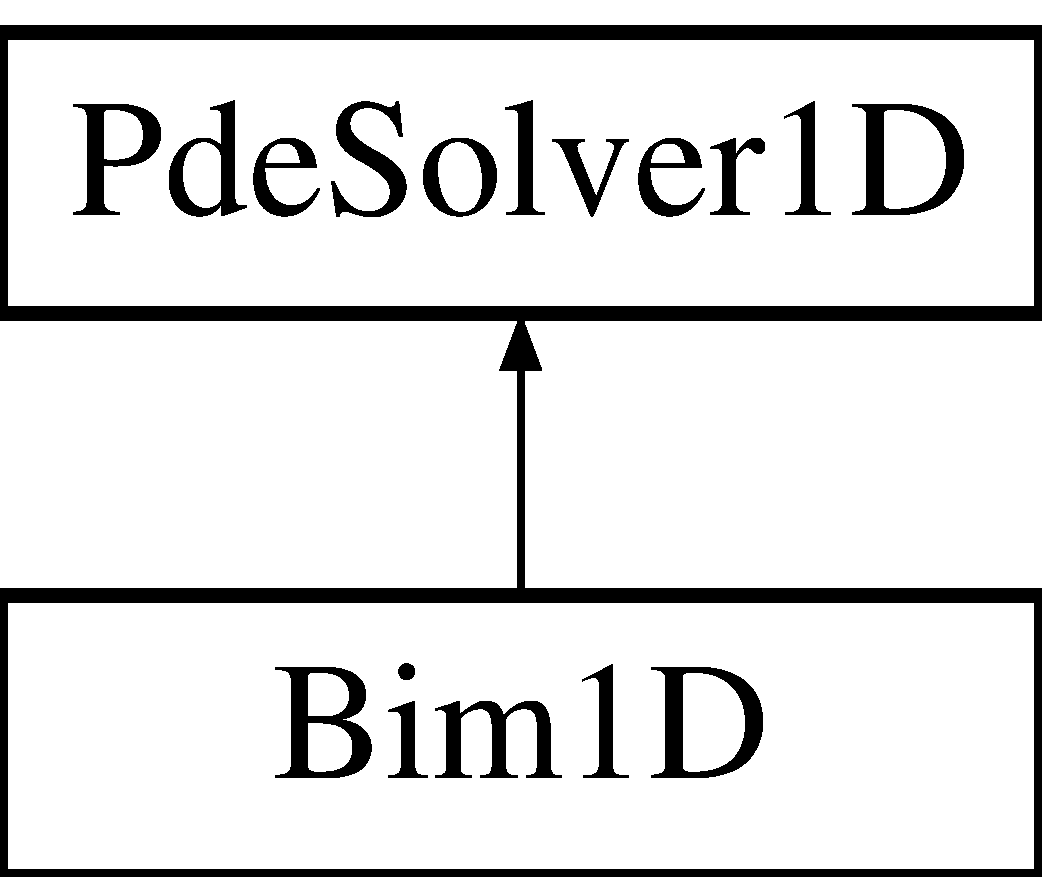
\includegraphics[height=2.000000cm]{classBim1D}
\end{center}
\end{figure}
\subsection*{Public Member Functions}
\begin{DoxyCompactItemize}
\item 
\hypertarget{classBim1D_aaa2cb4f70036268c64965b09be0ee721}{\hyperlink{classBim1D_aaa2cb4f70036268c64965b09be0ee721}{Bim1\-D} ()=delete}\label{classBim1D_aaa2cb4f70036268c64965b09be0ee721}

\begin{DoxyCompactList}\small\item\em Default constructor (deleted since it is required to specify the mesh). \end{DoxyCompactList}\item 
\hyperlink{classBim1D_a54ee6a3d7e3ebf52392f80800e31241c}{Bim1\-D} (\hyperlink{typedefs_8h_aae6cee78ed9cd8f234ed8cb48682548a}{Vector\-Xr} \&)
\begin{DoxyCompactList}\small\item\em Constructor. \end{DoxyCompactList}\item 
\hypertarget{classBim1D_a2fa6995307b37f25bf3c047a959e8b5a}{virtual \hyperlink{classBim1D_a2fa6995307b37f25bf3c047a959e8b5a}{$\sim$\-Bim1\-D} ()=default}\label{classBim1D_a2fa6995307b37f25bf3c047a959e8b5a}

\begin{DoxyCompactList}\small\item\em Destructor (defaulted). \end{DoxyCompactList}\item 
virtual void \hyperlink{classBim1D_a87a3b65a453d6fee3aa04e0b63b3b16d}{assemble\-Adv\-Diff} (const \hyperlink{typedefs_8h_aae6cee78ed9cd8f234ed8cb48682548a}{Vector\-Xr} \&, const \hyperlink{typedefs_8h_aae6cee78ed9cd8f234ed8cb48682548a}{Vector\-Xr} \&, const \hyperlink{typedefs_8h_aae6cee78ed9cd8f234ed8cb48682548a}{Vector\-Xr} \&, const \hyperlink{typedefs_8h_aae6cee78ed9cd8f234ed8cb48682548a}{Vector\-Xr} \&) override
\begin{DoxyCompactList}\small\item\em Assemble the matrix for an advection-\/diffusion term. \end{DoxyCompactList}\item 
virtual void \hyperlink{classBim1D_a9afebaa0bb7d919ece20a533ef000921}{assemble\-Stiff} (const \hyperlink{typedefs_8h_aae6cee78ed9cd8f234ed8cb48682548a}{Vector\-Xr} \&, const \hyperlink{typedefs_8h_aae6cee78ed9cd8f234ed8cb48682548a}{Vector\-Xr} \&) override
\begin{DoxyCompactList}\small\item\em Assemble the matrix for a diffusion term. \end{DoxyCompactList}\item 
virtual void \hyperlink{classBim1D_afd5e07bb246bdacd59eefb7a3396e650}{assemble\-Mass} (const \hyperlink{typedefs_8h_aae6cee78ed9cd8f234ed8cb48682548a}{Vector\-Xr} \&, const \hyperlink{typedefs_8h_aae6cee78ed9cd8f234ed8cb48682548a}{Vector\-Xr} \&) override
\begin{DoxyCompactList}\small\item\em Assemble the matrix for a reaction term. \end{DoxyCompactList}\end{DoxyCompactItemize}
\subsection*{Static Public Member Functions}
\begin{DoxyCompactItemize}
\item 
static \hyperlink{typedefs_8h_aae6cee78ed9cd8f234ed8cb48682548a}{Vector\-Xr} \hyperlink{classBim1D_a303a753f955d8733960429064c425331}{log\-\_\-mean} (const \hyperlink{typedefs_8h_aae6cee78ed9cd8f234ed8cb48682548a}{Vector\-Xr} \&, const \hyperlink{typedefs_8h_aae6cee78ed9cd8f234ed8cb48682548a}{Vector\-Xr} \&)
\begin{DoxyCompactList}\small\item\em Compute the element-\/wise logarithmic mean of two vectors. \end{DoxyCompactList}\item 
static std\-::pair$<$ \hyperlink{typedefs_8h_aae6cee78ed9cd8f234ed8cb48682548a}{Vector\-Xr}, \\*
\hyperlink{typedefs_8h_aae6cee78ed9cd8f234ed8cb48682548a}{Vector\-Xr} $>$ \hyperlink{classBim1D_aefd0ddeec3502f3a505ff18aec525925}{bernoulli} (const \hyperlink{typedefs_8h_aae6cee78ed9cd8f234ed8cb48682548a}{Vector\-Xr} \&)
\begin{DoxyCompactList}\small\item\em Compute the values of the Bernoulli function. \end{DoxyCompactList}\end{DoxyCompactItemize}
\subsection*{Additional Inherited Members}


\subsection{Detailed Description}
Class derived from \hyperlink{classPdeSolver1D}{Pde\-Solver1\-D}, providing a finite volume Box Integration Method (B\-I\-M) solver. 

Matrices are held in a sparse format. 

Definition at line 115 of file solvers.\-h.



\subsection{Constructor \& Destructor Documentation}
\hypertarget{classBim1D_a54ee6a3d7e3ebf52392f80800e31241c}{\index{Bim1\-D@{Bim1\-D}!Bim1\-D@{Bim1\-D}}
\index{Bim1\-D@{Bim1\-D}!Bim1D@{Bim1\-D}}
\subsubsection[{Bim1\-D}]{\setlength{\rightskip}{0pt plus 5cm}{\bf Bim1\-D} (
\begin{DoxyParamCaption}
\item[{{\bf Vector\-Xr} \&}]{mesh}
\end{DoxyParamCaption}
)}}\label{classBim1D_a54ee6a3d7e3ebf52392f80800e31241c}


Constructor. 


\begin{DoxyParams}[1]{Parameters}
\mbox{\tt in}  & {\em mesh} & \-: the mesh coordinates. \\
\hline
\end{DoxyParams}


Definition at line 18 of file solvers.\-cc.



\subsection{Member Function Documentation}
\hypertarget{classBim1D_a303a753f955d8733960429064c425331}{\index{Bim1\-D@{Bim1\-D}!log\-\_\-mean@{log\-\_\-mean}}
\index{log\-\_\-mean@{log\-\_\-mean}!Bim1D@{Bim1\-D}}
\subsubsection[{log\-\_\-mean}]{\setlength{\rightskip}{0pt plus 5cm}{\bf Vector\-Xr} log\-\_\-mean (
\begin{DoxyParamCaption}
\item[{const {\bf Vector\-Xr} \&}]{x1, }
\item[{const {\bf Vector\-Xr} \&}]{x2}
\end{DoxyParamCaption}
)\hspace{0.3cm}{\ttfamily [static]}}}\label{classBim1D_a303a753f955d8733960429064c425331}


Compute the element-\/wise logarithmic mean of two vectors. 

\[ M_{log}(x_1, x_2) = \frac{x_2 - x_1}{\log{x_2} - \log{x_1}} = \frac{x_2 - x_1}{\log\left(\frac{x_2}{x_1}\right)} ~ .\] 
\begin{DoxyParams}[1]{Parameters}
\mbox{\tt in}  & {\em x1} & \-: the first vector; \\
\hline
\mbox{\tt in}  & {\em x2} & \-: the second vector. \\
\hline
\end{DoxyParams}
\begin{DoxyReturn}{Returns}
the vector of the logarithmic means. 
\end{DoxyReturn}


Definition at line 21 of file solvers.\-cc.

\hypertarget{classBim1D_aefd0ddeec3502f3a505ff18aec525925}{\index{Bim1\-D@{Bim1\-D}!bernoulli@{bernoulli}}
\index{bernoulli@{bernoulli}!Bim1D@{Bim1\-D}}
\subsubsection[{bernoulli}]{\setlength{\rightskip}{0pt plus 5cm}std\-::pair$<$ {\bf Vector\-Xr}, {\bf Vector\-Xr} $>$ bernoulli (
\begin{DoxyParamCaption}
\item[{const {\bf Vector\-Xr} \&}]{x}
\end{DoxyParamCaption}
)\hspace{0.3cm}{\ttfamily [static]}}}\label{classBim1D_aefd0ddeec3502f3a505ff18aec525925}


Compute the values of the Bernoulli function. 

\[ \mathfrak{B}(x) = \frac{x}{e^x - 1} ~ .\] 
\begin{DoxyParams}[1]{Parameters}
\mbox{\tt in}  & {\em x} & \-: the vector of the values to compute the Bernoulli function at. \\
\hline
\end{DoxyParams}
\begin{DoxyReturn}{Returns}
the pair $ \left(\mathfrak{B}(x), \mathfrak{B}(-x)\right) $. 
\end{DoxyReturn}


Definition at line 52 of file solvers.\-cc.

\hypertarget{classBim1D_a87a3b65a453d6fee3aa04e0b63b3b16d}{\index{Bim1\-D@{Bim1\-D}!assemble\-Adv\-Diff@{assemble\-Adv\-Diff}}
\index{assemble\-Adv\-Diff@{assemble\-Adv\-Diff}!Bim1D@{Bim1\-D}}
\subsubsection[{assemble\-Adv\-Diff}]{\setlength{\rightskip}{0pt plus 5cm}void assemble\-Adv\-Diff (
\begin{DoxyParamCaption}
\item[{const {\bf Vector\-Xr} \&}]{alpha, }
\item[{const {\bf Vector\-Xr} \&}]{gamma, }
\item[{const {\bf Vector\-Xr} \&}]{eta, }
\item[{const {\bf Vector\-Xr} \&}]{beta}
\end{DoxyParamCaption}
)\hspace{0.3cm}{\ttfamily [override]}, {\ttfamily [virtual]}}}\label{classBim1D_a87a3b65a453d6fee3aa04e0b63b3b16d}


Assemble the matrix for an advection-\/diffusion term. 

Build the Scharfetter-\/\-Gummel stabilized stiffness matrix for\-: $ -\nabla\cdot\left(\alpha\cdot\gamma\left(\eta\nabla u - \beta u\right)\right) = f $.


\begin{DoxyParams}[1]{Parameters}
\mbox{\tt in}  & {\em alpha} & \-: $ \alpha $, an element-\/wise constant function; \\
\hline
\mbox{\tt in}  & {\em gamma} & \-: $ \gamma $, an element-\/wise linear function; \\
\hline
\mbox{\tt in}  & {\em eta} & \-: $ \eta $, an element-\/wise linear function; \\
\hline
\mbox{\tt in}  & {\em beta} & \-: $ \beta $, an element-\/wise constant function. \\
\hline
\end{DoxyParams}


Implements \hyperlink{classPdeSolver1D_a8eef3ec8fa2d444e8d0d1815d81e81f9}{Pde\-Solver1\-D}.



Definition at line 111 of file solvers.\-cc.

\hypertarget{classBim1D_a9afebaa0bb7d919ece20a533ef000921}{\index{Bim1\-D@{Bim1\-D}!assemble\-Stiff@{assemble\-Stiff}}
\index{assemble\-Stiff@{assemble\-Stiff}!Bim1D@{Bim1\-D}}
\subsubsection[{assemble\-Stiff}]{\setlength{\rightskip}{0pt plus 5cm}void assemble\-Stiff (
\begin{DoxyParamCaption}
\item[{const {\bf Vector\-Xr} \&}]{eps, }
\item[{const {\bf Vector\-Xr} \&}]{kappa}
\end{DoxyParamCaption}
)\hspace{0.3cm}{\ttfamily [override]}, {\ttfamily [virtual]}}}\label{classBim1D_a9afebaa0bb7d919ece20a533ef000921}


Assemble the matrix for a diffusion term. 

Build the standard finite element stiffness matrix for the diffusion problem\-: $ -\nabla\cdot\left(\epsilon\cdot\kappa\nabla u\right) = f $.


\begin{DoxyParams}[1]{Parameters}
\mbox{\tt in}  & {\em eps} & \-: $ \epsilon $, an element-\/wise constant function; \\
\hline
\mbox{\tt in}  & {\em kappa} & \-: $ \kappa $, an element-\/wise linear function. \\
\hline
\end{DoxyParams}


Implements \hyperlink{classPdeSolver1D_a0283447d8d645afde9fadb6adf224ee5}{Pde\-Solver1\-D}.



Definition at line 171 of file solvers.\-cc.

\hypertarget{classBim1D_afd5e07bb246bdacd59eefb7a3396e650}{\index{Bim1\-D@{Bim1\-D}!assemble\-Mass@{assemble\-Mass}}
\index{assemble\-Mass@{assemble\-Mass}!Bim1D@{Bim1\-D}}
\subsubsection[{assemble\-Mass}]{\setlength{\rightskip}{0pt plus 5cm}void assemble\-Mass (
\begin{DoxyParamCaption}
\item[{const {\bf Vector\-Xr} \&}]{delta, }
\item[{const {\bf Vector\-Xr} \&}]{zeta}
\end{DoxyParamCaption}
)\hspace{0.3cm}{\ttfamily [override]}, {\ttfamily [virtual]}}}\label{classBim1D_afd5e07bb246bdacd59eefb7a3396e650}


Assemble the matrix for a reaction term. 

Build the lumped finite element mass matrix for the reaction problem\-: $ \delta\cdot\zeta u = f $.


\begin{DoxyParams}[1]{Parameters}
\mbox{\tt in}  & {\em delta} & \-: $ \delta $, an element-\/wise constant function; \\
\hline
\mbox{\tt in}  & {\em zeta} & \-: $ \zeta $, an element-\/wise linear function. \\
\hline
\end{DoxyParams}


Implements \hyperlink{classPdeSolver1D_aa3dadbe748bfb8b897425e46500ab33b}{Pde\-Solver1\-D}.



Definition at line 180 of file solvers.\-cc.



The documentation for this class was generated from the following files\-:\begin{DoxyCompactItemize}
\item 
/home/elauksap/\-Dropbox/\-Progetto-\/\-P\-A\-C\-S/\-C++/\-Source/src/\hyperlink{solvers_8h}{solvers.\-h}\item 
/home/elauksap/\-Dropbox/\-Progetto-\/\-P\-A\-C\-S/\-C++/\-Source/src/\hyperlink{solvers_8cc}{solvers.\-cc}\end{DoxyCompactItemize}

\hypertarget{classCharge}{\section{Charge Class Reference}
\label{classCharge}\index{Charge@{Charge}}
}


Abstract class providing methods to calculate total electric charge (the rhs in the Poisson equation).  




{\ttfamily \#include $<$charge.\-h$>$}

Inheritance diagram for Charge\-:\begin{figure}[H]
\begin{center}
\leavevmode
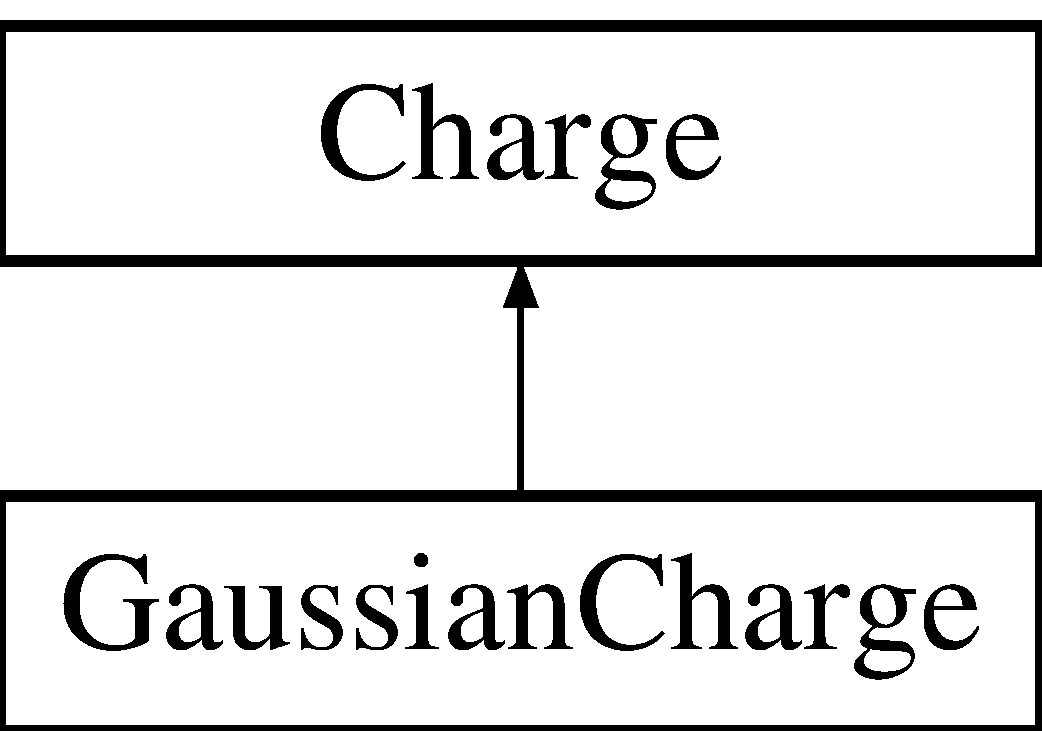
\includegraphics[height=2.000000cm]{classCharge}
\end{center}
\end{figure}
\subsection*{Public Member Functions}
\begin{DoxyCompactItemize}
\item 
\hypertarget{classCharge_ad8bd7ca1f5eb4af83b0457a01aeeb001}{\hyperlink{classCharge_ad8bd7ca1f5eb4af83b0457a01aeeb001}{Charge} ()=delete}\label{classCharge_ad8bd7ca1f5eb4af83b0457a01aeeb001}

\begin{DoxyCompactList}\small\item\em Default constructor (deleted since it is required to specify a \hyperlink{classParamList}{Param\-List} and a \hyperlink{classQuadratureRule}{Quadrature\-Rule}). \end{DoxyCompactList}\item 
\hyperlink{classCharge_a447211f3a5181d4efb8f2c7f1012c32b}{Charge} (const \hyperlink{classParamList}{Param\-List} \&, const \hyperlink{classQuadratureRule}{Quadrature\-Rule} \&)
\begin{DoxyCompactList}\small\item\em Constructor. \end{DoxyCompactList}\item 
\hypertarget{classCharge_ad350b0cd3356862aacbf538e6cffac61}{virtual \hyperlink{classCharge_ad350b0cd3356862aacbf538e6cffac61}{$\sim$\-Charge} ()=default}\label{classCharge_ad350b0cd3356862aacbf538e6cffac61}

\begin{DoxyCompactList}\small\item\em Destructor (defaulted). \end{DoxyCompactList}\item 
virtual \hyperlink{typedefs_8h_aae6cee78ed9cd8f234ed8cb48682548a}{Vector\-Xr} \hyperlink{classCharge_a597abd6d429e1c18935e4806082d67d8}{charge} (const \hyperlink{typedefs_8h_aae6cee78ed9cd8f234ed8cb48682548a}{Vector\-Xr} \&phi)=0
\begin{DoxyCompactList}\small\item\em Compute the total charge. \end{DoxyCompactList}\item 
virtual \hyperlink{typedefs_8h_aae6cee78ed9cd8f234ed8cb48682548a}{Vector\-Xr} \hyperlink{classCharge_acd71b3197f9081512d70d96ac694a3fc}{dcharge} (const \hyperlink{typedefs_8h_aae6cee78ed9cd8f234ed8cb48682548a}{Vector\-Xr} \&phi)=0
\begin{DoxyCompactList}\small\item\em Compute the derivative of the total charge with respect to the electric potential. \end{DoxyCompactList}\end{DoxyCompactItemize}
\subsection*{Protected Attributes}
\begin{DoxyCompactItemize}
\item 
\hypertarget{classCharge_a98166e75a7ce8273bfedf02e87bfd15f}{const \hyperlink{classParamList}{Param\-List} \& \hyperlink{classCharge_a98166e75a7ce8273bfedf02e87bfd15f}{params\-\_\-}}\label{classCharge_a98166e75a7ce8273bfedf02e87bfd15f}

\begin{DoxyCompactList}\small\item\em Parameter list handler. \end{DoxyCompactList}\item 
\hypertarget{classCharge_a37ca7d0fb67d7144675a97f8e4cbdf34}{const \hyperlink{classQuadratureRule}{Quadrature\-Rule} \& \hyperlink{classCharge_a37ca7d0fb67d7144675a97f8e4cbdf34}{rule\-\_\-}}\label{classCharge_a37ca7d0fb67d7144675a97f8e4cbdf34}

\begin{DoxyCompactList}\small\item\em Quadrature rule handler. \end{DoxyCompactList}\end{DoxyCompactItemize}


\subsection{Detailed Description}
Abstract class providing methods to calculate total electric charge (the rhs in the Poisson equation). 

Definition at line 28 of file charge.\-h.



\subsection{Constructor \& Destructor Documentation}
\hypertarget{classCharge_a447211f3a5181d4efb8f2c7f1012c32b}{\index{Charge@{Charge}!Charge@{Charge}}
\index{Charge@{Charge}!Charge@{Charge}}
\subsubsection[{Charge}]{\setlength{\rightskip}{0pt plus 5cm}{\bf Charge} (
\begin{DoxyParamCaption}
\item[{const {\bf Param\-List} \&}]{params, }
\item[{const {\bf Quadrature\-Rule} \&}]{rule}
\end{DoxyParamCaption}
)}}\label{classCharge_a447211f3a5181d4efb8f2c7f1012c32b}


Constructor. 


\begin{DoxyParams}[1]{Parameters}
\mbox{\tt in}  & {\em params} & \-: the list of simulation parameters; \\
\hline
\mbox{\tt in}  & {\em rule} & \-: a quadrature rule. \\
\hline
\end{DoxyParams}


Definition at line 17 of file charge.\-cc.



\subsection{Member Function Documentation}
\hypertarget{classCharge_a597abd6d429e1c18935e4806082d67d8}{\index{Charge@{Charge}!charge@{charge}}
\index{charge@{charge}!Charge@{Charge}}
\subsubsection[{charge}]{\setlength{\rightskip}{0pt plus 5cm}virtual {\bf Vector\-Xr} charge (
\begin{DoxyParamCaption}
\item[{const {\bf Vector\-Xr} \&}]{phi}
\end{DoxyParamCaption}
)\hspace{0.3cm}{\ttfamily [pure virtual]}}}\label{classCharge_a597abd6d429e1c18935e4806082d67d8}


Compute the total charge. 


\begin{DoxyParams}[1]{Parameters}
\mbox{\tt in}  & {\em phi} & \-: the electric potential $ \varphi $. \\
\hline
\end{DoxyParams}
\begin{DoxyReturn}{Returns}
the total charge $ q \left[ C \right] $. 
\end{DoxyReturn}


Implemented in \hyperlink{classExponentialCharge_a97ff25e546dee1ee5fec866b290ec999}{Exponential\-Charge}, and \hyperlink{classGaussianCharge_a97ff25e546dee1ee5fec866b290ec999}{Gaussian\-Charge}.

\hypertarget{classCharge_acd71b3197f9081512d70d96ac694a3fc}{\index{Charge@{Charge}!dcharge@{dcharge}}
\index{dcharge@{dcharge}!Charge@{Charge}}
\subsubsection[{dcharge}]{\setlength{\rightskip}{0pt plus 5cm}virtual {\bf Vector\-Xr} dcharge (
\begin{DoxyParamCaption}
\item[{const {\bf Vector\-Xr} \&}]{phi}
\end{DoxyParamCaption}
)\hspace{0.3cm}{\ttfamily [pure virtual]}}}\label{classCharge_acd71b3197f9081512d70d96ac694a3fc}


Compute the derivative of the total charge with respect to the electric potential. 


\begin{DoxyParams}[1]{Parameters}
\mbox{\tt in}  & {\em phi} & \-: the electric potential $ \varphi $. \\
\hline
\end{DoxyParams}
\begin{DoxyReturn}{Returns}
the derivative\-: $ \frac{\mathrm{d}q}{\mathrm{d}\varphi} \left[ C \cdot V^{-1} \right] $. 
\end{DoxyReturn}


Implemented in \hyperlink{classExponentialCharge_a06f7a60ee2bce4590e2a12286aa0e9eb}{Exponential\-Charge}, and \hyperlink{classGaussianCharge_a06f7a60ee2bce4590e2a12286aa0e9eb}{Gaussian\-Charge}.



The documentation for this class was generated from the following files\-:\begin{DoxyCompactItemize}
\item 
/home/elauksap/\-Dropbox/\-Progetto-\/\-P\-A\-C\-S/\-C++/\-Source/src/\hyperlink{charge_8h}{charge.\-h}\item 
/home/elauksap/\-Dropbox/\-Progetto-\/\-P\-A\-C\-S/\-C++/\-Source/src/\hyperlink{charge_8cc}{charge.\-cc}\end{DoxyCompactItemize}

\hypertarget{classCsvParser}{\section{Csv\-Parser Class Reference}
\label{classCsvParser}\index{Csv\-Parser@{Csv\-Parser}}
}


Class providing methods to read {\bfseries numeric} content from a .csv file and to store it in \hyperlink{index_Eigen}{Eigen} matrices or vectors.  




{\ttfamily \#include $<$csv\-Parser.\-h$>$}

\subsection*{Public Member Functions}
\begin{DoxyCompactItemize}
\item 
\hypertarget{classCsvParser_a9694abc21c2bc6d593a2489f6896ca10}{\hyperlink{classCsvParser_a9694abc21c2bc6d593a2489f6896ca10}{Csv\-Parser} ()=delete}\label{classCsvParser_a9694abc21c2bc6d593a2489f6896ca10}

\begin{DoxyCompactList}\small\item\em Default constructor (deleted since it is required to specify at least a filename). \end{DoxyCompactList}\item 
\hyperlink{classCsvParser_a928811b407ea6816bab9fef75d504301}{Csv\-Parser} (const std\-::string \&, const bool \&=true)
\begin{DoxyCompactList}\small\item\em Constructor\-: load the input file and check its compatibility with the code. \end{DoxyCompactList}\item 
\hypertarget{classCsvParser_a73aa36f7e9a832f184c98873c930e83e}{virtual \hyperlink{classCsvParser_a73aa36f7e9a832f184c98873c930e83e}{$\sim$\-Csv\-Parser} ()}\label{classCsvParser_a73aa36f7e9a832f184c98873c930e83e}

\begin{DoxyCompactList}\small\item\em Destructor\-: close the input file. \end{DoxyCompactList}\item 
\hyperlink{typedefs_8h_aaf38a491cc6d8aeb1c1f53f380789bad}{Row\-Vector\-Xr} \hyperlink{classCsvParser_a480e8570942d68f55cfae439e210e46e}{import\-Row} (const \hyperlink{typedefs_8h_a2c726f8f32697958e9d6c2afecda531d}{Index} \&)
\begin{DoxyCompactList}\small\item\em Method to import a row from the input file. \end{DoxyCompactList}\item 
\hyperlink{typedefs_8h_a81d507f5d0c665fb16966595c9520a55}{Matrix\-Xr} \hyperlink{classCsvParser_a42817812d475d6a42dee592d5854b297}{import\-Rows} (const std\-::initializer\-\_\-list$<$ \hyperlink{typedefs_8h_a2c726f8f32697958e9d6c2afecda531d}{Index} $>$ \&)
\begin{DoxyCompactList}\small\item\em Method to import multiple rows from the input file. \end{DoxyCompactList}\item 
\hyperlink{typedefs_8h_a81d507f5d0c665fb16966595c9520a55}{Matrix\-Xr} \hyperlink{classCsvParser_ad061e2e592b0f2d1b1f33c12fe0424d6}{import\-First\-Rows} (const \hyperlink{typedefs_8h_a2c726f8f32697958e9d6c2afecda531d}{Index} \&)
\begin{DoxyCompactList}\small\item\em Method to import the first {\itshape n\-Rows} rows from the input file. \end{DoxyCompactList}\item 
\hyperlink{typedefs_8h_aae6cee78ed9cd8f234ed8cb48682548a}{Vector\-Xr} \hyperlink{classCsvParser_ade7034e1a9dba4299e53a96d27aa836e}{import\-Col} (const \hyperlink{typedefs_8h_a2c726f8f32697958e9d6c2afecda531d}{Index} \&)
\begin{DoxyCompactList}\small\item\em Method to import a column from the input file. \end{DoxyCompactList}\item 
\hyperlink{typedefs_8h_a81d507f5d0c665fb16966595c9520a55}{Matrix\-Xr} \hyperlink{classCsvParser_a02ae981df8f4b1e9d5878a7be6a0c867}{import\-Cols} (const std\-::initializer\-\_\-list$<$ \hyperlink{typedefs_8h_a2c726f8f32697958e9d6c2afecda531d}{Index} $>$ \&)
\begin{DoxyCompactList}\small\item\em Method to import multiple columns from the input file. \end{DoxyCompactList}\item 
\hyperlink{typedefs_8h_a81d507f5d0c665fb16966595c9520a55}{Matrix\-Xr} \hyperlink{classCsvParser_a98bb8475e310605adc492fdd942d4347}{import\-First\-Cols} (const \hyperlink{typedefs_8h_a2c726f8f32697958e9d6c2afecda531d}{Index} \&)
\begin{DoxyCompactList}\small\item\em Method to import the first {\itshape n\-Cols} columns from the input file. \end{DoxyCompactList}\item 
\hyperlink{typedefs_8h_a060b837c3b4486ee35317744156f3da2}{Real} \hyperlink{classCsvParser_ab55ce0b3da48508e006698bb639d90a2}{import\-Cell} (const \hyperlink{typedefs_8h_a2c726f8f32697958e9d6c2afecda531d}{Index} \&, const \hyperlink{typedefs_8h_a2c726f8f32697958e9d6c2afecda531d}{Index} \&)
\begin{DoxyCompactList}\small\item\em Method to import a single cell from the input file. \end{DoxyCompactList}\item 
\hyperlink{typedefs_8h_a81d507f5d0c665fb16966595c9520a55}{Matrix\-Xr} \hyperlink{classCsvParser_a603c6845e97f53719d61319e45c188a9}{import\-All} ()
\begin{DoxyCompactList}\small\item\em Method to import the whole input file. \end{DoxyCompactList}\end{DoxyCompactItemize}
\begin{Indent}{\bf Getter methods}\par
\begin{DoxyCompactItemize}
\item 
\hypertarget{classCsvParser_ac7ea83f67eb1df8778c2408eae5adfc3}{const \hyperlink{typedefs_8h_a2c726f8f32697958e9d6c2afecda531d}{Index} \& {\bfseries n\-Rows} () const }\label{classCsvParser_ac7ea83f67eb1df8778c2408eae5adfc3}

\item 
\hypertarget{classCsvParser_a883f9a29fb05649de4212acf808dbde4}{const \hyperlink{typedefs_8h_a2c726f8f32697958e9d6c2afecda531d}{Index} \& {\bfseries n\-Cols} () const }\label{classCsvParser_a883f9a29fb05649de4212acf808dbde4}

\end{DoxyCompactItemize}
\end{Indent}
\subsection*{Private Member Functions}
\begin{DoxyCompactItemize}
\item 
\hypertarget{classCsvParser_ad20897c5c8bd47f5d4005989bead0e55}{void \hyperlink{classCsvParser_ad20897c5c8bd47f5d4005989bead0e55}{reset} ()}\label{classCsvParser_ad20897c5c8bd47f5d4005989bead0e55}

\begin{DoxyCompactList}\small\item\em Reset all the flags for {\itshape input\-\_\-} and go back to the beginning of file (possibly by ignoring headers). \end{DoxyCompactList}\end{DoxyCompactItemize}
\subsection*{Private Attributes}
\begin{DoxyCompactItemize}
\item 
\hypertarget{classCsvParser_abd8b856c78fe3ce8b32f1e6b0a390c84}{bool \hyperlink{classCsvParser_abd8b856c78fe3ce8b32f1e6b0a390c84}{has\-Headers\-\_\-}}\label{classCsvParser_abd8b856c78fe3ce8b32f1e6b0a390c84}

\begin{DoxyCompactList}\small\item\em bool to determine if first row contains headers or not. \end{DoxyCompactList}\item 
\hypertarget{classCsvParser_ad62252c05d21acdbb51ce29623efe9da}{\hyperlink{typedefs_8h_a2c726f8f32697958e9d6c2afecda531d}{Index} \hyperlink{classCsvParser_ad62252c05d21acdbb51ce29623efe9da}{n\-Rows\-\_\-}}\label{classCsvParser_ad62252c05d21acdbb51ce29623efe9da}

\begin{DoxyCompactList}\small\item\em Number of rows in the input file. \end{DoxyCompactList}\item 
\hypertarget{classCsvParser_aec28145f095ecbfb8dcec7a7fb90c382}{\hyperlink{typedefs_8h_a2c726f8f32697958e9d6c2afecda531d}{Index} \hyperlink{classCsvParser_aec28145f095ecbfb8dcec7a7fb90c382}{n\-Cols\-\_\-}}\label{classCsvParser_aec28145f095ecbfb8dcec7a7fb90c382}

\begin{DoxyCompactList}\small\item\em Number of columns in the input file. \end{DoxyCompactList}\item 
\hypertarget{classCsvParser_a418665bb33ded4f1ce88bedb60e3ffc0}{std\-::ifstream \hyperlink{classCsvParser_a418665bb33ded4f1ce88bedb60e3ffc0}{input\-\_\-}}\label{classCsvParser_a418665bb33ded4f1ce88bedb60e3ffc0}

\begin{DoxyCompactList}\small\item\em Input stream to {\itshape input\-\_\-filename}. \end{DoxyCompactList}\item 
\hypertarget{classCsvParser_aaeb353f8e1c649830268cfa5635eaa4f}{std\-::string \hyperlink{classCsvParser_aaeb353f8e1c649830268cfa5635eaa4f}{line\-\_\-}}\label{classCsvParser_aaeb353f8e1c649830268cfa5635eaa4f}

\begin{DoxyCompactList}\small\item\em Auxiliary variable to store currently processed line. \end{DoxyCompactList}\item 
\hypertarget{classCsvParser_a650afe260de7540becd03fd198dd1a59}{char \hyperlink{classCsvParser_a650afe260de7540becd03fd198dd1a59}{separator\-\_\-}}\label{classCsvParser_a650afe260de7540becd03fd198dd1a59}

\begin{DoxyCompactList}\small\item\em The separator character detected. \end{DoxyCompactList}\end{DoxyCompactItemize}


\subsection{Detailed Description}
Class providing methods to read {\bfseries numeric} content from a .csv file and to store it in \hyperlink{index_Eigen}{Eigen} matrices or vectors. 

Definition at line 32 of file csv\-Parser.\-h.



\subsection{Constructor \& Destructor Documentation}
\hypertarget{classCsvParser_a928811b407ea6816bab9fef75d504301}{\index{Csv\-Parser@{Csv\-Parser}!Csv\-Parser@{Csv\-Parser}}
\index{Csv\-Parser@{Csv\-Parser}!CsvParser@{Csv\-Parser}}
\subsubsection[{Csv\-Parser}]{\setlength{\rightskip}{0pt plus 5cm}{\bf Csv\-Parser} (
\begin{DoxyParamCaption}
\item[{const std\-::string \&}]{input\-\_\-filename, }
\item[{const bool \&}]{has\-Headers = {\ttfamily true}}
\end{DoxyParamCaption}
)}}\label{classCsvParser_a928811b407ea6816bab9fef75d504301}


Constructor\-: load the input file and check its compatibility with the code. 


\begin{DoxyParams}[1]{Parameters}
\mbox{\tt in}  & {\em input\-\_\-filename} & \-: the name of the input file; \\
\hline
\mbox{\tt in}  & {\em has\-Headers} & \-: bool to specify if first row contains headers or not; if {\bfseries true}, first row is always ignored. \\
\hline
\end{DoxyParams}


Definition at line 22 of file csv\-Parser.\-cc.



\subsection{Member Function Documentation}
\hypertarget{classCsvParser_a480e8570942d68f55cfae439e210e46e}{\index{Csv\-Parser@{Csv\-Parser}!import\-Row@{import\-Row}}
\index{import\-Row@{import\-Row}!CsvParser@{Csv\-Parser}}
\subsubsection[{import\-Row}]{\setlength{\rightskip}{0pt plus 5cm}{\bf Row\-Vector\-Xr} import\-Row (
\begin{DoxyParamCaption}
\item[{const {\bf Index} \&}]{index}
\end{DoxyParamCaption}
)}}\label{classCsvParser_a480e8570942d68f55cfae439e210e46e}


Method to import a row from the input file. 


\begin{DoxyParams}[1]{Parameters}
\mbox{\tt in}  & {\em index} & \-: the row index. \\
\hline
\end{DoxyParams}
\begin{DoxyReturn}{Returns}
a row vector containing the content read. 
\end{DoxyReturn}


Definition at line 93 of file csv\-Parser.\-cc.

\hypertarget{classCsvParser_a42817812d475d6a42dee592d5854b297}{\index{Csv\-Parser@{Csv\-Parser}!import\-Rows@{import\-Rows}}
\index{import\-Rows@{import\-Rows}!CsvParser@{Csv\-Parser}}
\subsubsection[{import\-Rows}]{\setlength{\rightskip}{0pt plus 5cm}{\bf Matrix\-Xr} import\-Rows (
\begin{DoxyParamCaption}
\item[{const std\-::initializer\-\_\-list$<$ {\bf Index} $>$ \&}]{indexes}
\end{DoxyParamCaption}
)}}\label{classCsvParser_a42817812d475d6a42dee592d5854b297}


Method to import multiple rows from the input file. 


\begin{DoxyParams}[1]{Parameters}
\mbox{\tt in}  & {\em indexes} & \-: initializer list containing the row indexes (e.\-g. something like \{1, 3, 4\}). \\
\hline
\end{DoxyParams}
\begin{DoxyReturn}{Returns}
a matrix containing the content read (row by row). 
\end{DoxyReturn}


Definition at line 124 of file csv\-Parser.\-cc.

\hypertarget{classCsvParser_ad061e2e592b0f2d1b1f33c12fe0424d6}{\index{Csv\-Parser@{Csv\-Parser}!import\-First\-Rows@{import\-First\-Rows}}
\index{import\-First\-Rows@{import\-First\-Rows}!CsvParser@{Csv\-Parser}}
\subsubsection[{import\-First\-Rows}]{\setlength{\rightskip}{0pt plus 5cm}{\bf Matrix\-Xr} import\-First\-Rows (
\begin{DoxyParamCaption}
\item[{const {\bf Index} \&}]{n\-Rows}
\end{DoxyParamCaption}
)}}\label{classCsvParser_ad061e2e592b0f2d1b1f33c12fe0424d6}


Method to import the first {\itshape n\-Rows} rows from the input file. 


\begin{DoxyParams}[1]{Parameters}
\mbox{\tt in}  & {\em n\-Rows} & \-: the number of rows to import. \\
\hline
\end{DoxyParams}
\begin{DoxyReturn}{Returns}
a matrix containing the content read (row by row). 
\end{DoxyReturn}


Definition at line 141 of file csv\-Parser.\-cc.

\hypertarget{classCsvParser_ade7034e1a9dba4299e53a96d27aa836e}{\index{Csv\-Parser@{Csv\-Parser}!import\-Col@{import\-Col}}
\index{import\-Col@{import\-Col}!CsvParser@{Csv\-Parser}}
\subsubsection[{import\-Col}]{\setlength{\rightskip}{0pt plus 5cm}{\bf Vector\-Xr} import\-Col (
\begin{DoxyParamCaption}
\item[{const {\bf Index} \&}]{index}
\end{DoxyParamCaption}
)}}\label{classCsvParser_ade7034e1a9dba4299e53a96d27aa836e}


Method to import a column from the input file. 


\begin{DoxyParams}[1]{Parameters}
\mbox{\tt in}  & {\em index} & \-: the column index. \\
\hline
\end{DoxyParams}
\begin{DoxyReturn}{Returns}
a column vector containing the content read. 
\end{DoxyReturn}


Definition at line 155 of file csv\-Parser.\-cc.

\hypertarget{classCsvParser_a02ae981df8f4b1e9d5878a7be6a0c867}{\index{Csv\-Parser@{Csv\-Parser}!import\-Cols@{import\-Cols}}
\index{import\-Cols@{import\-Cols}!CsvParser@{Csv\-Parser}}
\subsubsection[{import\-Cols}]{\setlength{\rightskip}{0pt plus 5cm}{\bf Matrix\-Xr} import\-Cols (
\begin{DoxyParamCaption}
\item[{const std\-::initializer\-\_\-list$<$ {\bf Index} $>$ \&}]{indexes}
\end{DoxyParamCaption}
)}}\label{classCsvParser_a02ae981df8f4b1e9d5878a7be6a0c867}


Method to import multiple columns from the input file. 


\begin{DoxyParams}[1]{Parameters}
\mbox{\tt in}  & {\em indexes} & \-: initializer list containing the column indexes (e.\-g. something like \{1, 3, 4\}). \\
\hline
\end{DoxyParams}
\begin{DoxyReturn}{Returns}
a matrix containing the content read (column by column). 
\end{DoxyReturn}


Definition at line 182 of file csv\-Parser.\-cc.

\hypertarget{classCsvParser_a98bb8475e310605adc492fdd942d4347}{\index{Csv\-Parser@{Csv\-Parser}!import\-First\-Cols@{import\-First\-Cols}}
\index{import\-First\-Cols@{import\-First\-Cols}!CsvParser@{Csv\-Parser}}
\subsubsection[{import\-First\-Cols}]{\setlength{\rightskip}{0pt plus 5cm}{\bf Matrix\-Xr} import\-First\-Cols (
\begin{DoxyParamCaption}
\item[{const {\bf Index} \&}]{n\-Cols}
\end{DoxyParamCaption}
)}}\label{classCsvParser_a98bb8475e310605adc492fdd942d4347}


Method to import the first {\itshape n\-Cols} columns from the input file. 


\begin{DoxyParams}[1]{Parameters}
\mbox{\tt in}  & {\em n\-Cols} & \-: the number of columns to import. \\
\hline
\end{DoxyParams}
\begin{DoxyReturn}{Returns}
a matrix containing the content read (column by column). 
\end{DoxyReturn}


Definition at line 199 of file csv\-Parser.\-cc.

\hypertarget{classCsvParser_ab55ce0b3da48508e006698bb639d90a2}{\index{Csv\-Parser@{Csv\-Parser}!import\-Cell@{import\-Cell}}
\index{import\-Cell@{import\-Cell}!CsvParser@{Csv\-Parser}}
\subsubsection[{import\-Cell}]{\setlength{\rightskip}{0pt plus 5cm}{\bf Real} import\-Cell (
\begin{DoxyParamCaption}
\item[{const {\bf Index} \&}]{row\-Index, }
\item[{const {\bf Index} \&}]{col\-Index}
\end{DoxyParamCaption}
)}}\label{classCsvParser_ab55ce0b3da48508e006698bb639d90a2}


Method to import a single cell from the input file. 


\begin{DoxyParams}[1]{Parameters}
\mbox{\tt in}  & {\em row\-Index} & \-: the cell row index. \\
\hline
\mbox{\tt in}  & {\em col\-Index} & \-: the cell column index. \\
\hline
\end{DoxyParams}
\begin{DoxyReturn}{Returns}
a scalar containing the value read. 
\end{DoxyReturn}


Definition at line 213 of file csv\-Parser.\-cc.

\hypertarget{classCsvParser_a603c6845e97f53719d61319e45c188a9}{\index{Csv\-Parser@{Csv\-Parser}!import\-All@{import\-All}}
\index{import\-All@{import\-All}!CsvParser@{Csv\-Parser}}
\subsubsection[{import\-All}]{\setlength{\rightskip}{0pt plus 5cm}{\bf Matrix\-Xr} import\-All (
\begin{DoxyParamCaption}
{}
\end{DoxyParamCaption}
)}}\label{classCsvParser_a603c6845e97f53719d61319e45c188a9}


Method to import the whole input file. 

\begin{DoxyReturn}{Returns}
a matrix containing the content read (cell by cell). 
\end{DoxyReturn}


Definition at line 221 of file csv\-Parser.\-cc.



The documentation for this class was generated from the following files\-:\begin{DoxyCompactItemize}
\item 
/home/elauksap/\-Dropbox/\-Progetto-\/\-P\-A\-C\-S/\-C++/\-Source/src/\hyperlink{csvParser_8h}{csv\-Parser.\-h}\item 
/home/elauksap/\-Dropbox/\-Progetto-\/\-P\-A\-C\-S/\-C++/\-Source/src/\hyperlink{csvParser_8cc}{csv\-Parser.\-cc}\end{DoxyCompactItemize}

\hypertarget{classDosModel}{\section{Dos\-Model Class Reference}
\label{classDosModel}\index{Dos\-Model@{Dos\-Model}}
}


Class providing methods to process a simulation to extract the Density of States starting from a parameter list.  




{\ttfamily \#include $<$dos\-Model.\-h$>$}



Collaboration diagram for Dos\-Model\-:\nopagebreak
\begin{figure}[H]
\begin{center}
\leavevmode
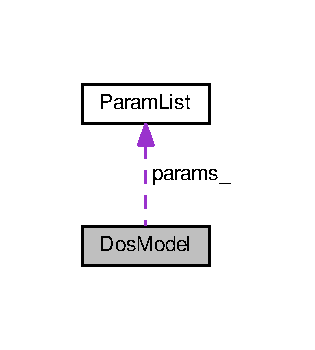
\includegraphics[width=151pt]{classDosModel__coll__graph}
\end{center}
\end{figure}
\subsection*{Public Member Functions}
\begin{DoxyCompactItemize}
\item 
\hypertarget{classDosModel_a500b55ef4d49a883dbe2ea137e85c839}{\hyperlink{classDosModel_a500b55ef4d49a883dbe2ea137e85c839}{Dos\-Model} ()}\label{classDosModel_a500b55ef4d49a883dbe2ea137e85c839}

\begin{DoxyCompactList}\small\item\em Default constructor. \end{DoxyCompactList}\item 
\hyperlink{classDosModel_a34d929790447adf8aae840519e1c8284}{Dos\-Model} (const \hyperlink{classParamList}{Param\-List} \&)
\begin{DoxyCompactList}\small\item\em Explicit conversion constructor. \end{DoxyCompactList}\item 
\hypertarget{classDosModel_a5361d0f34ccc062eef4564226f765aee}{virtual \hyperlink{classDosModel_a5361d0f34ccc062eef4564226f765aee}{$\sim$\-Dos\-Model} ()=default}\label{classDosModel_a5361d0f34ccc062eef4564226f765aee}

\begin{DoxyCompactList}\small\item\em Destructor (defaulted). \end{DoxyCompactList}\item 
\hypertarget{classDosModel_a5fd763c7e4ba5d643fdaa061ff3c506a}{const \hyperlink{classParamList}{Param\-List} \& \hyperlink{classDosModel_a5fd763c7e4ba5d643fdaa061ff3c506a}{params} () const }\label{classDosModel_a5fd763c7e4ba5d643fdaa061ff3c506a}

\begin{DoxyCompactList}\small\item\em Getter method. \end{DoxyCompactList}\item 
void \hyperlink{classDosModel_a8c3fc92853bec19ee326ceaf3fb0dd9c}{simulate} (const Get\-Pot \&, const std\-::string \&, const std\-::string \&, const std\-::string \&, const std\-::string \&)
\begin{DoxyCompactList}\small\item\em Perform the simulation. \end{DoxyCompactList}\item 
void \hyperlink{classDosModel_a7c242ffcdb811bb6378ac14fa113c18f}{post\-\_\-process} (const Get\-Pot \&, const std\-::string \&, std\-::ostream \&, std\-::ostream \&, const \hyperlink{typedefs_8h_a060b837c3b4486ee35317744156f3da2}{Real} \&, const \hyperlink{typedefs_8h_a060b837c3b4486ee35317744156f3da2}{Real} \&, const \hyperlink{typedefs_8h_aae6cee78ed9cd8f234ed8cb48682548a}{Vector\-Xr} \&, const \hyperlink{typedefs_8h_aae6cee78ed9cd8f234ed8cb48682548a}{Vector\-Xr} \&, const \hyperlink{typedefs_8h_aae6cee78ed9cd8f234ed8cb48682548a}{Vector\-Xr} \&, const \hyperlink{typedefs_8h_aae6cee78ed9cd8f234ed8cb48682548a}{Vector\-Xr} \&)
\begin{DoxyCompactList}\small\item\em Perform post-\/processing. \end{DoxyCompactList}\item 
void \hyperlink{classDosModel_a26e64253688b5b51ffc54013bf3bc553}{gnuplot\-\_\-commands} (const std\-::string \&, std\-::ostream \&) const 
\begin{DoxyCompactList}\small\item\em Defines commands to generate \hyperlink{index_Gnuplot}{Gnuplot} output files. \end{DoxyCompactList}\item 
void \hyperlink{classDosModel_aa614583c066c644e83085beaad05279d}{save\-\_\-plot} (const std\-::string \&, const std\-::string \&, const std\-::string \&, const std\-::string \&) const 
\begin{DoxyCompactList}\small\item\em Save the \hyperlink{index_Gnuplot}{Gnuplot} output files. \end{DoxyCompactList}\end{DoxyCompactItemize}
\subsection*{Private Attributes}
\begin{DoxyCompactItemize}
\item 
\hypertarget{classDosModel_aef7436a220692b5b863db4e9d8b870a3}{bool \hyperlink{classDosModel_aef7436a220692b5b863db4e9d8b870a3}{initialized\-\_\-}}\label{classDosModel_aef7436a220692b5b863db4e9d8b870a3}

\begin{DoxyCompactList}\small\item\em bool to determine if \hyperlink{classDosModel}{Dos\-Model} {\itshape param\-\_\-} has been properly initialized. \end{DoxyCompactList}\item 
\hypertarget{classDosModel_a4deb2401e648f5ad79e0aab68343a96b}{\hyperlink{classParamList}{Param\-List} \hyperlink{classDosModel_a4deb2401e648f5ad79e0aab68343a96b}{params\-\_\-}}\label{classDosModel_a4deb2401e648f5ad79e0aab68343a96b}

\begin{DoxyCompactList}\small\item\em The parameter list. \end{DoxyCompactList}\item 
\hypertarget{classDosModel_afd8e6e3c2312d733b446fce08daf48e9}{\hyperlink{typedefs_8h_a060b837c3b4486ee35317744156f3da2}{Real} \hyperlink{classDosModel_afd8e6e3c2312d733b446fce08daf48e9}{V\-\_\-shift\-\_\-}}\label{classDosModel_afd8e6e3c2312d733b446fce08daf48e9}

\begin{DoxyCompactList}\small\item\em Peak shift between experimental data and simulated values $ [V] $. \end{DoxyCompactList}\end{DoxyCompactItemize}


\subsection{Detailed Description}
Class providing methods to process a simulation to extract the Density of States starting from a parameter list. 

Definition at line 42 of file dos\-Model.\-h.



\subsection{Constructor \& Destructor Documentation}
\hypertarget{classDosModel_a34d929790447adf8aae840519e1c8284}{\index{Dos\-Model@{Dos\-Model}!Dos\-Model@{Dos\-Model}}
\index{Dos\-Model@{Dos\-Model}!DosModel@{Dos\-Model}}
\subsubsection[{Dos\-Model}]{\setlength{\rightskip}{0pt plus 5cm}{\bf Dos\-Model} (
\begin{DoxyParamCaption}
\item[{const {\bf Param\-List} \&}]{params}
\end{DoxyParamCaption}
)\hspace{0.3cm}{\ttfamily [explicit]}}}\label{classDosModel_a34d929790447adf8aae840519e1c8284}


Explicit conversion constructor. 


\begin{DoxyParams}[1]{Parameters}
\mbox{\tt in}  & {\em params} & \-: a parameter list. \\
\hline
\end{DoxyParams}


Definition at line 24 of file dos\-Model.\-cc.



\subsection{Member Function Documentation}
\hypertarget{classDosModel_a8c3fc92853bec19ee326ceaf3fb0dd9c}{\index{Dos\-Model@{Dos\-Model}!simulate@{simulate}}
\index{simulate@{simulate}!DosModel@{Dos\-Model}}
\subsubsection[{simulate}]{\setlength{\rightskip}{0pt plus 5cm}void simulate (
\begin{DoxyParamCaption}
\item[{const Get\-Pot \&}]{config, }
\item[{const std\-::string \&}]{input\-\_\-experim, }
\item[{const std\-::string \&}]{output\-\_\-directory, }
\item[{const std\-::string \&}]{output\-\_\-plot\-\_\-subdir, }
\item[{const std\-::string \&}]{output\-\_\-filename}
\end{DoxyParamCaption}
)}}\label{classDosModel_a8c3fc92853bec19ee326ceaf3fb0dd9c}


Perform the simulation. 


\begin{DoxyParams}[1]{Parameters}
\mbox{\tt in}  & {\em config} & \-: the Get\-Pot configuration object; \\
\hline
\mbox{\tt in}  & {\em input\-\_\-experim} & \-: the file containing experimental data; \\
\hline
\mbox{\tt in}  & {\em output\-\_\-directory} & \-: directory where to store output files; \\
\hline
\mbox{\tt in}  & {\em output\-\_\-plot\-\_\-subdir} & \-: sub-\/directory where to store \hyperlink{index_Gnuplot}{Gnuplot} files; \\
\hline
\mbox{\tt in}  & {\em output\-\_\-filename} & \-: prefix for the output filename. \\
\hline
\end{DoxyParams}


Definition at line 27 of file dos\-Model.\-cc.

\hypertarget{classDosModel_a7c242ffcdb811bb6378ac14fa113c18f}{\index{Dos\-Model@{Dos\-Model}!post\-\_\-process@{post\-\_\-process}}
\index{post\-\_\-process@{post\-\_\-process}!DosModel@{Dos\-Model}}
\subsubsection[{post\-\_\-process}]{\setlength{\rightskip}{0pt plus 5cm}void post\-\_\-process (
\begin{DoxyParamCaption}
\item[{const Get\-Pot \&}]{config, }
\item[{const std\-::string \&}]{input\-\_\-experim, }
\item[{std\-::ostream \&}]{output\-\_\-fitting, }
\item[{std\-::ostream \&}]{output\-\_\-\-C\-V, }
\item[{const {\bf Real} \&}]{A\-\_\-semic, }
\item[{const {\bf Real} \&}]{C\-\_\-sb, }
\item[{const {\bf Vector\-Xr} \&}]{x\-\_\-semic, }
\item[{const {\bf Vector\-Xr} \&}]{dens, }
\item[{const {\bf Vector\-Xr} \&}]{V\-\_\-simulated, }
\item[{const {\bf Vector\-Xr} \&}]{C\-\_\-simulated}
\end{DoxyParamCaption}
)}}\label{classDosModel_a7c242ffcdb811bb6378ac14fa113c18f}


Perform post-\/processing. 


\begin{DoxyParams}[1]{Parameters}
\mbox{\tt in}  & {\em config} & \-: the Get\-Pot configuration object; \\
\hline
\mbox{\tt in}  & {\em input\-\_\-experim} & \-: the file containing experimental data; \\
\hline
\mbox{\tt out}  & {\em output\-\_\-fitting} & \-: output file containing infos about fitting experimental data; \\
\hline
\mbox{\tt out}  & {\em output\-\_\-\-C\-V} & \-: output file containing infos about capacitance-\/voltage data; \\
\hline
\mbox{\tt in}  & {\em A\-\_\-semic} & \-: area of the semiconductor; \\
\hline
\mbox{\tt in}  & {\em C\-\_\-sb} & \-: stray border capacitance (see \hyperlink{classParamList}{Param\-List}); \\
\hline
\mbox{\tt in}  & {\em x\-\_\-semic} & \-: the mesh corresponding to the semiconductor domain; \\
\hline
\mbox{\tt in}  & {\em dens} & \-: charge density $ \left[ C \cdot m^{-3} \right] $; \\
\hline
\mbox{\tt in}  & {\em V\-\_\-simulated} & \-: simulated voltage values; \\
\hline
\mbox{\tt in}  & {\em C\-\_\-simulated} & \-: simulated capacitance values. \\
\hline
\end{DoxyParams}


Definition at line 273 of file dos\-Model.\-cc.

\hypertarget{classDosModel_a26e64253688b5b51ffc54013bf3bc553}{\index{Dos\-Model@{Dos\-Model}!gnuplot\-\_\-commands@{gnuplot\-\_\-commands}}
\index{gnuplot\-\_\-commands@{gnuplot\-\_\-commands}!DosModel@{Dos\-Model}}
\subsubsection[{gnuplot\-\_\-commands}]{\setlength{\rightskip}{0pt plus 5cm}void gnuplot\-\_\-commands (
\begin{DoxyParamCaption}
\item[{const std\-::string \&}]{output\-\_\-\-C\-V\-\_\-filename, }
\item[{std\-::ostream \&}]{os}
\end{DoxyParamCaption}
) const}}\label{classDosModel_a26e64253688b5b51ffc54013bf3bc553}


Defines commands to generate \hyperlink{index_Gnuplot}{Gnuplot} output files. 


\begin{DoxyParams}[1]{Parameters}
\mbox{\tt in}  & {\em output\-\_\-\-C\-V\-\_\-filename} & \-: output C\-V filename; \\
\hline
\mbox{\tt out}  & {\em os} & \-: output stream. \\
\hline
\end{DoxyParams}


Definition at line 364 of file dos\-Model.\-cc.

\hypertarget{classDosModel_aa614583c066c644e83085beaad05279d}{\index{Dos\-Model@{Dos\-Model}!save\-\_\-plot@{save\-\_\-plot}}
\index{save\-\_\-plot@{save\-\_\-plot}!DosModel@{Dos\-Model}}
\subsubsection[{save\-\_\-plot}]{\setlength{\rightskip}{0pt plus 5cm}void save\-\_\-plot (
\begin{DoxyParamCaption}
\item[{const std\-::string \&}]{output\-\_\-directory, }
\item[{const std\-::string \&}]{output\-\_\-plot\-\_\-subdir, }
\item[{const std\-::string \&}]{output\-\_\-\-C\-V\-\_\-filename, }
\item[{const std\-::string \&}]{output\-\_\-filename}
\end{DoxyParamCaption}
) const}}\label{classDosModel_aa614583c066c644e83085beaad05279d}


Save the \hyperlink{index_Gnuplot}{Gnuplot} output files. 


\begin{DoxyParams}[1]{Parameters}
\mbox{\tt in}  & {\em output\-\_\-directory} & \-: directory where to store output files; \\
\hline
\mbox{\tt in}  & {\em output\-\_\-plot\-\_\-subdir} & \-: sub-\/directory where to store \hyperlink{index_Gnuplot}{Gnuplot} files; \\
\hline
\mbox{\tt in}  & {\em output\-\_\-\-C\-V\-\_\-filename} & \-: output C\-V filename; \\
\hline
\mbox{\tt in}  & {\em output\-\_\-filename} & \-: prefix for the output filename. \\
\hline
\end{DoxyParams}


Definition at line 398 of file dos\-Model.\-cc.



The documentation for this class was generated from the following files\-:\begin{DoxyCompactItemize}
\item 
Dos\-Extraction/src/\hyperlink{dosModel_8h}{dos\-Model.\-h}\item 
Dos\-Extraction/src/\hyperlink{dosModel_8cc}{dos\-Model.\-cc}\end{DoxyCompactItemize}

\hypertarget{classGaussHermiteRule}{\section{Gauss\-Hermite\-Rule Class Reference}
\label{classGaussHermiteRule}\index{Gauss\-Hermite\-Rule@{Gauss\-Hermite\-Rule}}
}


Class derived from \hyperlink{classQuadratureRule}{Quadrature\-Rule} providing the Gauss-\/\-Hermite quadrature rule.  




{\ttfamily \#include $<$quadrature\-Rule.\-h$>$}



Inheritance diagram for Gauss\-Hermite\-Rule\-:\nopagebreak
\begin{figure}[H]
\begin{center}
\leavevmode
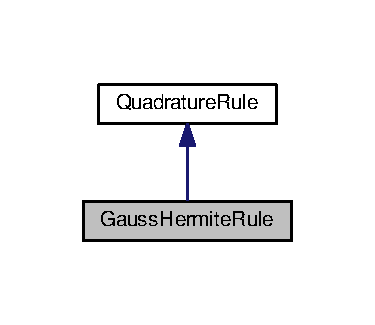
\includegraphics[width=180pt]{classGaussHermiteRule__inherit__graph}
\end{center}
\end{figure}


Collaboration diagram for Gauss\-Hermite\-Rule\-:\nopagebreak
\begin{figure}[H]
\begin{center}
\leavevmode
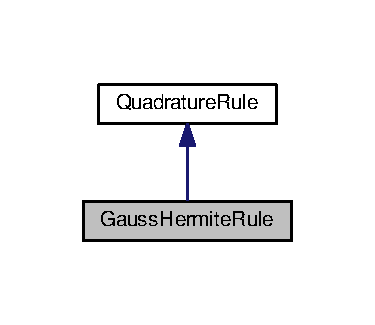
\includegraphics[width=180pt]{classGaussHermiteRule__coll__graph}
\end{center}
\end{figure}
\subsection*{Public Member Functions}
\begin{DoxyCompactItemize}
\item 
\hypertarget{classGaussHermiteRule_a82318908e412ac924a27d7c816c5e89d}{\hyperlink{classGaussHermiteRule_a82318908e412ac924a27d7c816c5e89d}{Gauss\-Hermite\-Rule} ()=delete}\label{classGaussHermiteRule_a82318908e412ac924a27d7c816c5e89d}

\begin{DoxyCompactList}\small\item\em Default constructor (deleted since it is required to specify the number of nodes). \end{DoxyCompactList}\item 
\hyperlink{classGaussHermiteRule_a650e19b8ef2851cdc955a1201b76f9b5}{Gauss\-Hermite\-Rule} (const \hyperlink{typedefs_8h_a2c726f8f32697958e9d6c2afecda531d}{Index} \&)
\begin{DoxyCompactList}\small\item\em Constructor. \end{DoxyCompactList}\item 
\hypertarget{classGaussHermiteRule_ade51ec8543da3071631a6e1dbf1ac9f7}{virtual \hyperlink{classGaussHermiteRule_ade51ec8543da3071631a6e1dbf1ac9f7}{$\sim$\-Gauss\-Hermite\-Rule} ()=default}\label{classGaussHermiteRule_ade51ec8543da3071631a6e1dbf1ac9f7}

\begin{DoxyCompactList}\small\item\em Destructor (defaulted). \end{DoxyCompactList}\item 
\hypertarget{classGaussHermiteRule_ae5502fed0f3128dce83d1280a834ffac}{virtual void \hyperlink{classGaussHermiteRule_ae5502fed0f3128dce83d1280a834ffac}{apply} () override}\label{classGaussHermiteRule_ae5502fed0f3128dce83d1280a834ffac}

\begin{DoxyCompactList}\small\item\em Apply the quadrature rule in order to compute the nodes and weights. \end{DoxyCompactList}\item 
virtual void \hyperlink{classGaussHermiteRule_a6265ae995213bef29d216da947f5f692}{apply} (const Get\-Pot \&) override
\begin{DoxyCompactList}\small\item\em Apply the quadrature rule reading parameters from a configuration file. \end{DoxyCompactList}\item 
\hypertarget{classGaussHermiteRule_a5a21a96592fcd473df6739c72c083063}{void \hyperlink{classGaussHermiteRule_a5a21a96592fcd473df6739c72c083063}{apply\-\_\-iterative\-\_\-algorithm} (const \hyperlink{typedefs_8h_a2c726f8f32697958e9d6c2afecda531d}{Index} \&=1000, const \hyperlink{typedefs_8h_a060b837c3b4486ee35317744156f3da2}{Real} \&=1.\-0e-\/14)}\label{classGaussHermiteRule_a5a21a96592fcd473df6739c72c083063}

\begin{DoxyCompactList}\small\item\em Compute nodes and weights using an adapted version of the algorithm presented in\-: \par
William H. Press, Saul A. Teukolsky, William T. Vetterling, and Brian P. Flannery. 2007. \par
Numerical Recipes\-: The Art of Scientific Computing (3rd edition). \par
Cambridge University Press, New York, N\-Y, U\-S\-A. \end{DoxyCompactList}\item 
\hypertarget{classGaussHermiteRule_add3939f72a845e748c388220bb1ad934}{void \hyperlink{classGaussHermiteRule_add3939f72a845e748c388220bb1ad934}{apply\-\_\-using\-\_\-eigendecomposition} ()}\label{classGaussHermiteRule_add3939f72a845e748c388220bb1ad934}

\begin{DoxyCompactList}\small\item\em Compute nodes and weights using an eigendecomposition-\/based algorithm. \end{DoxyCompactList}\end{DoxyCompactItemize}
\subsection*{Additional Inherited Members}


\subsection{Detailed Description}
Class derived from \hyperlink{classQuadratureRule}{Quadrature\-Rule} providing the Gauss-\/\-Hermite quadrature rule. 

Compute nodes and weights for the {\itshape n\-Nodes\-\_\-}-\/points approximation of\-: \[ \int_{-\infty}^{+\infty} w(x)f(x)~\mathrm{d}x \] where $ w(x) = e^{-x^2} $. 

Definition at line 94 of file quadrature\-Rule.\-h.



\subsection{Constructor \& Destructor Documentation}
\hypertarget{classGaussHermiteRule_a650e19b8ef2851cdc955a1201b76f9b5}{\index{Gauss\-Hermite\-Rule@{Gauss\-Hermite\-Rule}!Gauss\-Hermite\-Rule@{Gauss\-Hermite\-Rule}}
\index{Gauss\-Hermite\-Rule@{Gauss\-Hermite\-Rule}!GaussHermiteRule@{Gauss\-Hermite\-Rule}}
\subsubsection[{Gauss\-Hermite\-Rule}]{\setlength{\rightskip}{0pt plus 5cm}{\bf Gauss\-Hermite\-Rule} (
\begin{DoxyParamCaption}
\item[{const {\bf Index} \&}]{n\-Nodes}
\end{DoxyParamCaption}
)}}\label{classGaussHermiteRule_a650e19b8ef2851cdc955a1201b76f9b5}


Constructor. 


\begin{DoxyParams}[1]{Parameters}
\mbox{\tt in}  & {\em n\-Nodes} & \-: the number of nodes to be used for the quadrature rule. \\
\hline
\end{DoxyParams}


Definition at line 28 of file quadrature\-Rule.\-cc.



\subsection{Member Function Documentation}
\hypertarget{classGaussHermiteRule_a6265ae995213bef29d216da947f5f692}{\index{Gauss\-Hermite\-Rule@{Gauss\-Hermite\-Rule}!apply@{apply}}
\index{apply@{apply}!GaussHermiteRule@{Gauss\-Hermite\-Rule}}
\subsubsection[{apply}]{\setlength{\rightskip}{0pt plus 5cm}void apply (
\begin{DoxyParamCaption}
\item[{const Get\-Pot \&}]{config}
\end{DoxyParamCaption}
)\hspace{0.3cm}{\ttfamily [override]}, {\ttfamily [virtual]}}}\label{classGaussHermiteRule_a6265ae995213bef29d216da947f5f692}


Apply the quadrature rule reading parameters from a configuration file. 


\begin{DoxyParams}[1]{Parameters}
\mbox{\tt in}  & {\em config} & \-: the Get\-Pot configuration object. \\
\hline
\end{DoxyParams}


Implements \hyperlink{classQuadratureRule_a0eac623f625d4faa872b1b031db76a75}{Quadrature\-Rule}.



Definition at line 36 of file quadrature\-Rule.\-cc.



The documentation for this class was generated from the following files\-:\begin{DoxyCompactItemize}
\item 
Dos\-Extraction/src/\hyperlink{quadratureRule_8h}{quadrature\-Rule.\-h}\item 
Dos\-Extraction/src/\hyperlink{quadratureRule_8cc}{quadrature\-Rule.\-cc}\end{DoxyCompactItemize}

\hypertarget{classGaussianCharge}{\section{Gaussian\-Charge Class Reference}
\label{classGaussianCharge}\index{Gaussian\-Charge@{Gaussian\-Charge}}
}


Class derived from \hyperlink{classCharge}{Charge}, under the hypothesis that Density of States is a combination of gaussians.  




{\ttfamily \#include $<$charge.\-h$>$}

Inheritance diagram for Gaussian\-Charge\-:\begin{figure}[H]
\begin{center}
\leavevmode
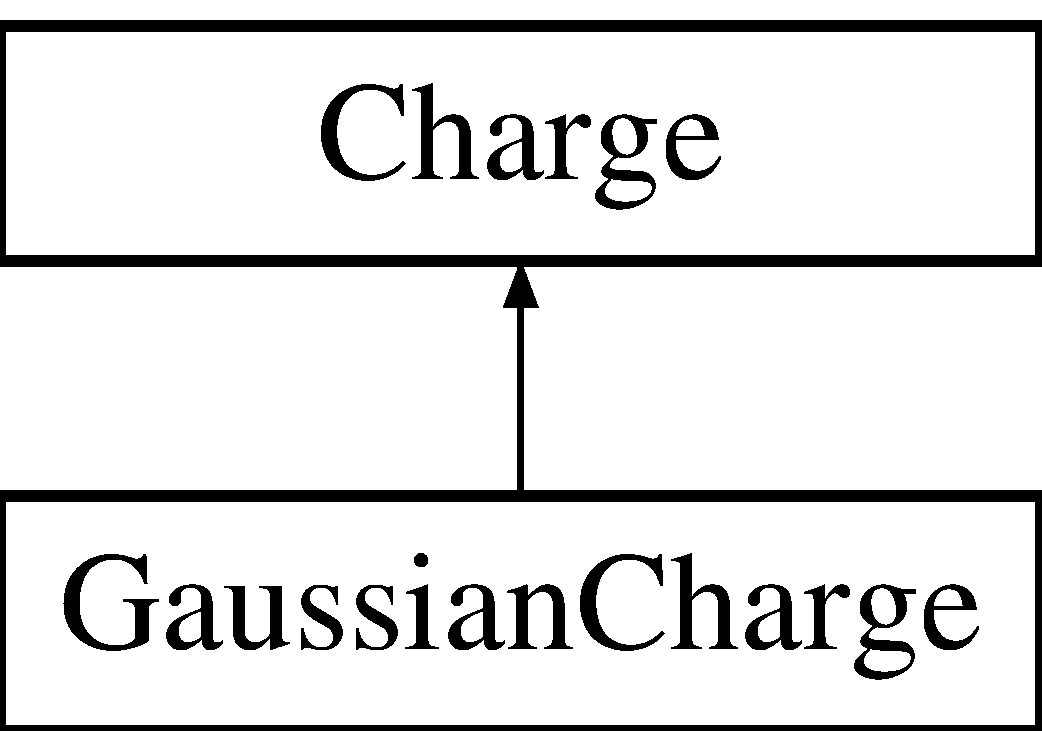
\includegraphics[height=2.000000cm]{classGaussianCharge}
\end{center}
\end{figure}
\subsection*{Public Member Functions}
\begin{DoxyCompactItemize}
\item 
\hypertarget{classGaussianCharge_a860db9bf8bccf98756f1f6bd60de5463}{\hyperlink{classGaussianCharge_a860db9bf8bccf98756f1f6bd60de5463}{Gaussian\-Charge} ()=delete}\label{classGaussianCharge_a860db9bf8bccf98756f1f6bd60de5463}

\begin{DoxyCompactList}\small\item\em Default constructor (deleted since it is required to specify a \hyperlink{classParamList}{Param\-List} and a \hyperlink{classQuadratureRule}{Quadrature\-Rule}). \end{DoxyCompactList}\item 
\hyperlink{classGaussianCharge_a3e5ff9c43a3deb7861ea10435de4bb55}{Gaussian\-Charge} (const \hyperlink{classParamList}{Param\-List} \&, const \hyperlink{classQuadratureRule}{Quadrature\-Rule} \&)
\begin{DoxyCompactList}\small\item\em Constructor. \end{DoxyCompactList}\item 
\hypertarget{classGaussianCharge_ab64872dfef0abc7d116d65373496ac33}{virtual \hyperlink{classGaussianCharge_ab64872dfef0abc7d116d65373496ac33}{$\sim$\-Gaussian\-Charge} ()=default}\label{classGaussianCharge_ab64872dfef0abc7d116d65373496ac33}

\begin{DoxyCompactList}\small\item\em Destructor (defaulted). \end{DoxyCompactList}\item 
virtual \hyperlink{typedefs_8h_aae6cee78ed9cd8f234ed8cb48682548a}{Vector\-Xr} \hyperlink{classGaussianCharge_a97ff25e546dee1ee5fec866b290ec999}{charge} (const \hyperlink{typedefs_8h_aae6cee78ed9cd8f234ed8cb48682548a}{Vector\-Xr} \&) override
\begin{DoxyCompactList}\small\item\em Compute the total charge. \end{DoxyCompactList}\item 
virtual \hyperlink{typedefs_8h_aae6cee78ed9cd8f234ed8cb48682548a}{Vector\-Xr} \hyperlink{classGaussianCharge_a06f7a60ee2bce4590e2a12286aa0e9eb}{dcharge} (const \hyperlink{typedefs_8h_aae6cee78ed9cd8f234ed8cb48682548a}{Vector\-Xr} \&) override
\begin{DoxyCompactList}\small\item\em Compute the derivative of the total charge with respect to the electric potential. \end{DoxyCompactList}\end{DoxyCompactItemize}
\subsection*{Private Member Functions}
\begin{DoxyCompactItemize}
\item 
\hyperlink{typedefs_8h_a060b837c3b4486ee35317744156f3da2}{Real} \hyperlink{classGaussianCharge_a91f27044b2f7ced7c2330153bb9da652}{n\-\_\-approx} (const \hyperlink{typedefs_8h_a060b837c3b4486ee35317744156f3da2}{Real} \&, const \hyperlink{typedefs_8h_a060b837c3b4486ee35317744156f3da2}{Real} \&, const \hyperlink{typedefs_8h_a060b837c3b4486ee35317744156f3da2}{Real} \&) const 
\begin{DoxyCompactList}\small\item\em Compute electrons density (per unit volume). \end{DoxyCompactList}\item 
\hyperlink{typedefs_8h_a060b837c3b4486ee35317744156f3da2}{Real} \hyperlink{classGaussianCharge_ab5ce245792f1b0d7c2038ebc75bbc758}{dn\-\_\-approx} (const \hyperlink{typedefs_8h_a060b837c3b4486ee35317744156f3da2}{Real} \&, const \hyperlink{typedefs_8h_a060b837c3b4486ee35317744156f3da2}{Real} \&, const \hyperlink{typedefs_8h_a060b837c3b4486ee35317744156f3da2}{Real} \&) const 
\begin{DoxyCompactList}\small\item\em Compute the approximate derivative of electrons density (per unit volume) with respect to the electric potential. \end{DoxyCompactList}\end{DoxyCompactItemize}
\subsection*{Additional Inherited Members}


\subsection{Detailed Description}
Class derived from \hyperlink{classCharge}{Charge}, under the hypothesis that Density of States is a combination of gaussians. 

Provide methods to compute total electric charge and its derivative under the hypothesis that Density of States is a linear combination of multiple gaussians, whose parameters are read from a \hyperlink{classParamList}{Param\-List} object, of the form\-: \[ \frac{N_0}{\sqrt{2\pi\sigma^2}}\exp\left(-\frac{\left(\cdot\right)^2}{2\sigma^2}\right) ~ . \] 

Definition at line 71 of file charge.\-h.



\subsection{Constructor \& Destructor Documentation}
\hypertarget{classGaussianCharge_a3e5ff9c43a3deb7861ea10435de4bb55}{\index{Gaussian\-Charge@{Gaussian\-Charge}!Gaussian\-Charge@{Gaussian\-Charge}}
\index{Gaussian\-Charge@{Gaussian\-Charge}!GaussianCharge@{Gaussian\-Charge}}
\subsubsection[{Gaussian\-Charge}]{\setlength{\rightskip}{0pt plus 5cm}{\bf Gaussian\-Charge} (
\begin{DoxyParamCaption}
\item[{const {\bf Param\-List} \&}]{params, }
\item[{const {\bf Quadrature\-Rule} \&}]{rule}
\end{DoxyParamCaption}
)}}\label{classGaussianCharge_a3e5ff9c43a3deb7861ea10435de4bb55}


Constructor. 


\begin{DoxyParams}[1]{Parameters}
\mbox{\tt in}  & {\em params} & \-: the list of simulation parameters; \\
\hline
\mbox{\tt in}  & {\em rule} & \-: a quadrature rule. \\
\hline
\end{DoxyParams}


Definition at line 17 of file charge.\-cc.



\subsection{Member Function Documentation}
\hypertarget{classGaussianCharge_a97ff25e546dee1ee5fec866b290ec999}{\index{Gaussian\-Charge@{Gaussian\-Charge}!charge@{charge}}
\index{charge@{charge}!GaussianCharge@{Gaussian\-Charge}}
\subsubsection[{charge}]{\setlength{\rightskip}{0pt plus 5cm}{\bf Vector\-Xr} charge (
\begin{DoxyParamCaption}
\item[{const {\bf Vector\-Xr} \&}]{phi}
\end{DoxyParamCaption}
)\hspace{0.3cm}{\ttfamily [override]}, {\ttfamily [virtual]}}}\label{classGaussianCharge_a97ff25e546dee1ee5fec866b290ec999}


Compute the total charge. 


\begin{DoxyParams}[1]{Parameters}
\mbox{\tt in}  & {\em phi} & \-: the electric potential $ \varphi $. \\
\hline
\end{DoxyParams}
\begin{DoxyReturn}{Returns}
the total charge $ q \left[ C \right] $. 
\end{DoxyReturn}


Implements \hyperlink{classCharge_a597abd6d429e1c18935e4806082d67d8}{Charge}.



Definition at line 48 of file charge.\-cc.

\hypertarget{classGaussianCharge_a06f7a60ee2bce4590e2a12286aa0e9eb}{\index{Gaussian\-Charge@{Gaussian\-Charge}!dcharge@{dcharge}}
\index{dcharge@{dcharge}!GaussianCharge@{Gaussian\-Charge}}
\subsubsection[{dcharge}]{\setlength{\rightskip}{0pt plus 5cm}{\bf Vector\-Xr} dcharge (
\begin{DoxyParamCaption}
\item[{const {\bf Vector\-Xr} \&}]{phi}
\end{DoxyParamCaption}
)\hspace{0.3cm}{\ttfamily [override]}, {\ttfamily [virtual]}}}\label{classGaussianCharge_a06f7a60ee2bce4590e2a12286aa0e9eb}


Compute the derivative of the total charge with respect to the electric potential. 


\begin{DoxyParams}[1]{Parameters}
\mbox{\tt in}  & {\em phi} & \-: the electric potential $ \varphi $. \\
\hline
\end{DoxyParams}
\begin{DoxyReturn}{Returns}
the derivative\-: $ \frac{\mathrm{d}q}{\mathrm{d}\varphi} \left[ C \cdot V^{-1} \right] $. 
\end{DoxyReturn}


Implements \hyperlink{classCharge_acd71b3197f9081512d70d96ac694a3fc}{Charge}.



Definition at line 75 of file charge.\-cc.

\hypertarget{classGaussianCharge_a91f27044b2f7ced7c2330153bb9da652}{\index{Gaussian\-Charge@{Gaussian\-Charge}!n\-\_\-approx@{n\-\_\-approx}}
\index{n\-\_\-approx@{n\-\_\-approx}!GaussianCharge@{Gaussian\-Charge}}
\subsubsection[{n\-\_\-approx}]{\setlength{\rightskip}{0pt plus 5cm}{\bf Real} n\-\_\-approx (
\begin{DoxyParamCaption}
\item[{const {\bf Real} \&}]{phi, }
\item[{const {\bf Real} \&}]{N0, }
\item[{const {\bf Real} \&}]{sigma}
\end{DoxyParamCaption}
) const\hspace{0.3cm}{\ttfamily [private]}}}\label{classGaussianCharge_a91f27044b2f7ced7c2330153bb9da652}


Compute electrons density (per unit volume). 


\begin{DoxyParams}[1]{Parameters}
\mbox{\tt in}  & {\em phi} & \-: the electric potential $ \varphi $; \\
\hline
\mbox{\tt in}  & {\em N0} & \-: the gaussian mean $ N_0 $; \\
\hline
\mbox{\tt in}  & {\em sigma} & \-: the gaussian standard deviation $ \sigma $. \\
\hline
\end{DoxyParams}
\begin{DoxyReturn}{Returns}
the electrons density $ n(\varphi) \left[ m^{-3} \right] $. 
\end{DoxyReturn}


Definition at line 20 of file charge.\-cc.

\hypertarget{classGaussianCharge_ab5ce245792f1b0d7c2038ebc75bbc758}{\index{Gaussian\-Charge@{Gaussian\-Charge}!dn\-\_\-approx@{dn\-\_\-approx}}
\index{dn\-\_\-approx@{dn\-\_\-approx}!GaussianCharge@{Gaussian\-Charge}}
\subsubsection[{dn\-\_\-approx}]{\setlength{\rightskip}{0pt plus 5cm}{\bf Real} dn\-\_\-approx (
\begin{DoxyParamCaption}
\item[{const {\bf Real} \&}]{phi, }
\item[{const {\bf Real} \&}]{N0, }
\item[{const {\bf Real} \&}]{sigma}
\end{DoxyParamCaption}
) const\hspace{0.3cm}{\ttfamily [private]}}}\label{classGaussianCharge_ab5ce245792f1b0d7c2038ebc75bbc758}


Compute the approximate derivative of electrons density (per unit volume) with respect to the electric potential. 


\begin{DoxyParams}[1]{Parameters}
\mbox{\tt in}  & {\em phi} & \-: the electric potential $ \varphi $; \\
\hline
\mbox{\tt in}  & {\em N0} & \-: the gaussian mean $ N_0 $; \\
\hline
\mbox{\tt in}  & {\em sigma} & \-: the gaussian standard deviation $ \sigma $. \\
\hline
\end{DoxyParams}
\begin{DoxyReturn}{Returns}
the derivative\-: $ \frac{\mathrm{d}n}{\mathrm{d}\varphi} \left[ m^{-3} \cdot V^{-1} \right] $. 
\end{DoxyReturn}


Definition at line 34 of file charge.\-cc.



The documentation for this class was generated from the following files\-:\begin{DoxyCompactItemize}
\item 
/home/elauksap/\-Dropbox/\-Progetto-\/\-P\-A\-C\-S/\-C++/\-Source/src/\hyperlink{charge_8h}{charge.\-h}\item 
/home/elauksap/\-Dropbox/\-Progetto-\/\-P\-A\-C\-S/\-C++/\-Source/src/\hyperlink{charge_8cc}{charge.\-cc}\end{DoxyCompactItemize}

\hypertarget{classNonLinearPoisson1D}{\section{Non\-Linear\-Poisson1\-D Class Reference}
\label{classNonLinearPoisson1D}\index{Non\-Linear\-Poisson1\-D@{Non\-Linear\-Poisson1\-D}}
}


Provide a solver for a non-\/linear Poisson equation.  




{\ttfamily \#include $<$solvers.\-h$>$}

\subsection*{Public Member Functions}
\begin{DoxyCompactItemize}
\item 
\hypertarget{classNonLinearPoisson1D_ad4d805d47a62331707176ad2693499f3}{\hyperlink{classNonLinearPoisson1D_ad4d805d47a62331707176ad2693499f3}{Non\-Linear\-Poisson1\-D} ()=delete}\label{classNonLinearPoisson1D_ad4d805d47a62331707176ad2693499f3}

\begin{DoxyCompactList}\small\item\em Default constructor (deleted since it is required to specify the solver to be used). \end{DoxyCompactList}\item 
\hyperlink{classNonLinearPoisson1D_ac6c77988b843e0bd9df82c97b7da7cf6}{Non\-Linear\-Poisson1\-D} (const \hyperlink{classPdeSolver1D}{Pde\-Solver1\-D} \&, const \hyperlink{typedefs_8h_a2c726f8f32697958e9d6c2afecda531d}{Index} \&=100, const \hyperlink{typedefs_8h_a060b837c3b4486ee35317744156f3da2}{Real} \&=1.\-0e-\/6)
\begin{DoxyCompactList}\small\item\em Constructor. \end{DoxyCompactList}\item 
\hypertarget{classNonLinearPoisson1D_a1452123e4787361491d2f54c46794df9}{virtual \hyperlink{classNonLinearPoisson1D_a1452123e4787361491d2f54c46794df9}{$\sim$\-Non\-Linear\-Poisson1\-D} ()=default}\label{classNonLinearPoisson1D_a1452123e4787361491d2f54c46794df9}

\begin{DoxyCompactList}\small\item\em Destructor (defaulted). \end{DoxyCompactList}\item 
void \hyperlink{classNonLinearPoisson1D_a54768475940b34c5e39583a3635cf63b}{apply} (const \hyperlink{typedefs_8h_aae6cee78ed9cd8f234ed8cb48682548a}{Vector\-Xr} \&, const \hyperlink{typedefs_8h_aae6cee78ed9cd8f234ed8cb48682548a}{Vector\-Xr} \&, \hyperlink{classCharge}{Charge} \&)
\begin{DoxyCompactList}\small\item\em Apply a Newton method to the equation and then discretize it using the solver specified. \end{DoxyCompactList}\end{DoxyCompactItemize}
\begin{Indent}{\bf Getter methods}\par
\begin{DoxyCompactItemize}
\item 
\hypertarget{classNonLinearPoisson1D_a49da0d6a457d7d2d996926ea813ec55f}{const \hyperlink{typedefs_8h_aae6cee78ed9cd8f234ed8cb48682548a}{Vector\-Xr} \& {\bfseries phi} () const }\label{classNonLinearPoisson1D_a49da0d6a457d7d2d996926ea813ec55f}

\item 
\hypertarget{classNonLinearPoisson1D_a146128a8e8cc2cad80edb7883e4823b8}{const \hyperlink{typedefs_8h_aae6cee78ed9cd8f234ed8cb48682548a}{Vector\-Xr} \& {\bfseries norm} () const }\label{classNonLinearPoisson1D_a146128a8e8cc2cad80edb7883e4823b8}

\item 
\hypertarget{classNonLinearPoisson1D_af46d2aa1358eab6b5d547cf40ba8a720}{const \hyperlink{typedefs_8h_a060b837c3b4486ee35317744156f3da2}{Real} \& {\bfseries q\-Tot} () const }\label{classNonLinearPoisson1D_af46d2aa1358eab6b5d547cf40ba8a720}

\item 
\hypertarget{classNonLinearPoisson1D_a341de5204baac856de6f8b6ed3721414}{const \hyperlink{typedefs_8h_a060b837c3b4486ee35317744156f3da2}{Real} \& {\bfseries c\-Tot} () const }\label{classNonLinearPoisson1D_a341de5204baac856de6f8b6ed3721414}

\end{DoxyCompactItemize}
\end{Indent}
\subsection*{Private Member Functions}
\begin{DoxyCompactItemize}
\item 
\hyperlink{typedefs_8h_a6d3b7db3fa8171d0e743df848524c269}{Sparse\-Xr} \hyperlink{classNonLinearPoisson1D_aeb48e911a352f4115f872f28a188b10a}{compute\-Jac} (const \hyperlink{typedefs_8h_aae6cee78ed9cd8f234ed8cb48682548a}{Vector\-Xr} \&) const 
\begin{DoxyCompactList}\small\item\em Compute the Jacobi matrix. \end{DoxyCompactList}\end{DoxyCompactItemize}
\subsection*{Private Attributes}
\begin{DoxyCompactItemize}
\item 
\hypertarget{classNonLinearPoisson1D_aca4acc679876b21bdbf4c09c589aed69}{const \hyperlink{classPdeSolver1D}{Pde\-Solver1\-D} \& \hyperlink{classNonLinearPoisson1D_aca4acc679876b21bdbf4c09c589aed69}{solver\-\_\-}}\label{classNonLinearPoisson1D_aca4acc679876b21bdbf4c09c589aed69}

\begin{DoxyCompactList}\small\item\em Solver handler. \end{DoxyCompactList}\item 
\hypertarget{classNonLinearPoisson1D_a6154a48301e532ef10ef6f1ceb6fa1c6}{\hyperlink{typedefs_8h_a2c726f8f32697958e9d6c2afecda531d}{Index} \hyperlink{classNonLinearPoisson1D_a6154a48301e532ef10ef6f1ceb6fa1c6}{max\-Iterations\-No\-\_\-}}\label{classNonLinearPoisson1D_a6154a48301e532ef10ef6f1ceb6fa1c6}

\begin{DoxyCompactList}\small\item\em Maximum number of iterations. \end{DoxyCompactList}\item 
\hypertarget{classNonLinearPoisson1D_a23d2944fdb4ac7f255b13aaa685af25d}{\hyperlink{typedefs_8h_a060b837c3b4486ee35317744156f3da2}{Real} \hyperlink{classNonLinearPoisson1D_a23d2944fdb4ac7f255b13aaa685af25d}{tolerance\-\_\-}}\label{classNonLinearPoisson1D_a23d2944fdb4ac7f255b13aaa685af25d}

\begin{DoxyCompactList}\small\item\em Tolerance. \end{DoxyCompactList}\item 
\hypertarget{classNonLinearPoisson1D_ad7990f1c65d985ae84833b7dde37f359}{\hyperlink{typedefs_8h_aae6cee78ed9cd8f234ed8cb48682548a}{Vector\-Xr} \hyperlink{classNonLinearPoisson1D_ad7990f1c65d985ae84833b7dde37f359}{phi\-\_\-}}\label{classNonLinearPoisson1D_ad7990f1c65d985ae84833b7dde37f359}

\begin{DoxyCompactList}\small\item\em The electric potential. \end{DoxyCompactList}\item 
\hypertarget{classNonLinearPoisson1D_a114ea11ef7ef7b96a627aced27fbe066}{\hyperlink{typedefs_8h_aae6cee78ed9cd8f234ed8cb48682548a}{Vector\-Xr} \hyperlink{classNonLinearPoisson1D_a114ea11ef7ef7b96a627aced27fbe066}{norm\-\_\-}}\label{classNonLinearPoisson1D_a114ea11ef7ef7b96a627aced27fbe066}

\begin{DoxyCompactList}\small\item\em Vector holding $ L^\infty $-\/norm errors for each iteration. \end{DoxyCompactList}\item 
\hypertarget{classNonLinearPoisson1D_a5fa713b8efdf7b2651478e560ae70074}{\hyperlink{typedefs_8h_a060b837c3b4486ee35317744156f3da2}{Real} \hyperlink{classNonLinearPoisson1D_a5fa713b8efdf7b2651478e560ae70074}{q\-Tot\-\_\-}}\label{classNonLinearPoisson1D_a5fa713b8efdf7b2651478e560ae70074}

\begin{DoxyCompactList}\small\item\em Total charge. \end{DoxyCompactList}\item 
\hypertarget{classNonLinearPoisson1D_a4edec5e6395e5a862df829a223323533}{\hyperlink{typedefs_8h_a060b837c3b4486ee35317744156f3da2}{Real} \hyperlink{classNonLinearPoisson1D_a4edec5e6395e5a862df829a223323533}{c\-Tot\-\_\-}}\label{classNonLinearPoisson1D_a4edec5e6395e5a862df829a223323533}

\begin{DoxyCompactList}\small\item\em Total capacitance. \end{DoxyCompactList}\end{DoxyCompactItemize}


\subsection{Detailed Description}
Provide a solver for a non-\/linear Poisson equation. 

A Newton method is applied in order to solve\-: \[ -\frac{\mathrm{d}}{\mathrm{d}z} \left(\epsilon(z) \cdot \frac{\mathrm{d}\varphi}{\mathrm{d}z}(z) \right) = - q \cdot \frac{N_0}{\sqrt{\pi}} \int_{-\infty}^{+\infty} \exp\left(-\alpha^2\right) \left( 1 + \exp\left( \frac{\sqrt{2}\sigma\alpha - q\varphi(z)}{K_B \cdot T} \right) \right)^{-1} \mathrm{d}\alpha ~ . \] 

Definition at line 189 of file solvers.\-h.



\subsection{Constructor \& Destructor Documentation}
\hypertarget{classNonLinearPoisson1D_ac6c77988b843e0bd9df82c97b7da7cf6}{\index{Non\-Linear\-Poisson1\-D@{Non\-Linear\-Poisson1\-D}!Non\-Linear\-Poisson1\-D@{Non\-Linear\-Poisson1\-D}}
\index{Non\-Linear\-Poisson1\-D@{Non\-Linear\-Poisson1\-D}!NonLinearPoisson1D@{Non\-Linear\-Poisson1\-D}}
\subsubsection[{Non\-Linear\-Poisson1\-D}]{\setlength{\rightskip}{0pt plus 5cm}{\bf Non\-Linear\-Poisson1\-D} (
\begin{DoxyParamCaption}
\item[{const {\bf Pde\-Solver1\-D} \&}]{solver, }
\item[{const {\bf Index} \&}]{max\-Iterations\-No = {\ttfamily 100}, }
\item[{const {\bf Real} \&}]{tolerance = {\ttfamily 1.0e-\/6}}
\end{DoxyParamCaption}
)}}\label{classNonLinearPoisson1D_ac6c77988b843e0bd9df82c97b7da7cf6}


Constructor. 


\begin{DoxyParams}[1]{Parameters}
\mbox{\tt in}  & {\em solver} & \-: the solver to be used; \\
\hline
\mbox{\tt in}  & {\em max\-Iterations\-No} & \-: maximum number of iterations desired; \\
\hline
\mbox{\tt in}  & {\em tolerance} & \-: tolerance desired. \\
\hline
\end{DoxyParams}


Definition at line 199 of file solvers.\-cc.



\subsection{Member Function Documentation}
\hypertarget{classNonLinearPoisson1D_a54768475940b34c5e39583a3635cf63b}{\index{Non\-Linear\-Poisson1\-D@{Non\-Linear\-Poisson1\-D}!apply@{apply}}
\index{apply@{apply}!NonLinearPoisson1D@{Non\-Linear\-Poisson1\-D}}
\subsubsection[{apply}]{\setlength{\rightskip}{0pt plus 5cm}void apply (
\begin{DoxyParamCaption}
\item[{const {\bf Vector\-Xr} \&}]{mesh, }
\item[{const {\bf Vector\-Xr} \&}]{init\-\_\-guess, }
\item[{{\bf Charge} \&}]{charge\-\_\-fun}
\end{DoxyParamCaption}
)}}\label{classNonLinearPoisson1D_a54768475940b34c5e39583a3635cf63b}


Apply a Newton method to the equation and then discretize it using the solver specified. 


\begin{DoxyParams}[1]{Parameters}
\mbox{\tt in}  & {\em mesh} & \-: the mesh; \\
\hline
\mbox{\tt in}  & {\em init\-\_\-guess} & \-: initial guess for the Newton algorithm; \\
\hline
\mbox{\tt in}  & {\em charge\-\_\-fun} & \-: an object of class \hyperlink{classCharge}{Charge} specifying how to compute total electric charge. \\
\hline
\end{DoxyParams}


Definition at line 206 of file solvers.\-cc.

\hypertarget{classNonLinearPoisson1D_aeb48e911a352f4115f872f28a188b10a}{\index{Non\-Linear\-Poisson1\-D@{Non\-Linear\-Poisson1\-D}!compute\-Jac@{compute\-Jac}}
\index{compute\-Jac@{compute\-Jac}!NonLinearPoisson1D@{Non\-Linear\-Poisson1\-D}}
\subsubsection[{compute\-Jac}]{\setlength{\rightskip}{0pt plus 5cm}{\bf Sparse\-Xr} compute\-Jac (
\begin{DoxyParamCaption}
\item[{const {\bf Vector\-Xr} \&}]{x}
\end{DoxyParamCaption}
) const\hspace{0.3cm}{\ttfamily [private]}}}\label{classNonLinearPoisson1D_aeb48e911a352f4115f872f28a188b10a}


Compute the Jacobi matrix. 


\begin{DoxyParams}[1]{Parameters}
\mbox{\tt in}  & {\em x} & \-: the vector where to start from. \\
\hline
\end{DoxyParams}
\begin{DoxyReturn}{Returns}
the Jacobi matrix in a sparse format. 
\end{DoxyReturn}


Definition at line 327 of file solvers.\-cc.



The documentation for this class was generated from the following files\-:\begin{DoxyCompactItemize}
\item 
/home/elauksap/\-Dropbox/\-Progetto-\/\-P\-A\-C\-S/\-C++/\-Source/src/\hyperlink{solvers_8h}{solvers.\-h}\item 
/home/elauksap/\-Dropbox/\-Progetto-\/\-P\-A\-C\-S/\-C++/\-Source/src/\hyperlink{solvers_8cc}{solvers.\-cc}\end{DoxyCompactItemize}

\hypertarget{classParamList}{\section{Param\-List Class Reference}
\label{classParamList}\index{Param\-List@{Param\-List}}
}


Class providing methods to handle a list of parameters.  




{\ttfamily \#include $<$param\-List.\-h$>$}

\subsection*{Public Member Functions}
\begin{DoxyCompactItemize}
\item 
\hypertarget{classParamList_a9e4b0ea6081bb500861f231f0b4f7900}{\hyperlink{classParamList_a9e4b0ea6081bb500861f231f0b4f7900}{Param\-List} ()=default}\label{classParamList_a9e4b0ea6081bb500861f231f0b4f7900}

\begin{DoxyCompactList}\small\item\em Default constructor (defaulted). \end{DoxyCompactList}\item 
\hyperlink{classParamList_a05bb961ce49e684edbae5f3f07f8b128}{Param\-List} (const Row\-Vector\-Xd \&)
\begin{DoxyCompactList}\small\item\em Explicit conversion constructor. \end{DoxyCompactList}\item 
\hypertarget{classParamList_a454ef9f83c9777b5c33cf273d88b3e5d}{virtual \hyperlink{classParamList_a454ef9f83c9777b5c33cf273d88b3e5d}{$\sim$\-Param\-List} ()=default}\label{classParamList_a454ef9f83c9777b5c33cf273d88b3e5d}

\begin{DoxyCompactList}\small\item\em Destructor (defaulted). \end{DoxyCompactList}\end{DoxyCompactItemize}
\begin{Indent}{\bf Getter methods}\par
\begin{DoxyCompactItemize}
\item 
\hypertarget{classParamList_a012be3a46bf086c10c0b8906b1c0ece1}{const unsigned \& {\bfseries simulation\-No} () const }\label{classParamList_a012be3a46bf086c10c0b8906b1c0ece1}

\item 
\hypertarget{classParamList_aaa4ab91dd1fb090f0d91a4c703e8c55a}{const double \& {\bfseries t\-\_\-semic} () const }\label{classParamList_aaa4ab91dd1fb090f0d91a4c703e8c55a}

\item 
\hypertarget{classParamList_a186672cc6a2eec77e726ab8337791822}{const double \& {\bfseries t\-\_\-ins} () const }\label{classParamList_a186672cc6a2eec77e726ab8337791822}

\item 
\hypertarget{classParamList_a4375bbd2e7ad0cede170a5ceb3f14bd0}{const double \& {\bfseries eps\-\_\-semic} () const }\label{classParamList_a4375bbd2e7ad0cede170a5ceb3f14bd0}

\item 
\hypertarget{classParamList_a26c5e5f7e2f9768a5dfb927ab2f27b0c}{const double \& {\bfseries eps\-\_\-ins} () const }\label{classParamList_a26c5e5f7e2f9768a5dfb927ab2f27b0c}

\item 
\hypertarget{classParamList_adcd107e7354e9fc5b74af7315fa7df80}{const double \& {\bfseries Wf} () const }\label{classParamList_adcd107e7354e9fc5b74af7315fa7df80}

\item 
\hypertarget{classParamList_a7bb2ca3a9d5d0c39b2236a9bcb3e0815}{const double \& {\bfseries Ea} () const }\label{classParamList_a7bb2ca3a9d5d0c39b2236a9bcb3e0815}

\item 
\hypertarget{classParamList_a208a97deee7c9c07aa4a24563c116b43}{const double \& {\bfseries N0} () const }\label{classParamList_a208a97deee7c9c07aa4a24563c116b43}

\item 
\hypertarget{classParamList_aeab76c5d57194aecd33538540db7c42f}{const double \& {\bfseries sigma} () const }\label{classParamList_aeab76c5d57194aecd33538540db7c42f}

\item 
\hypertarget{classParamList_af17ca56cc73a7ebadb577308bd5b7ad6}{const double \& {\bfseries N0\-\_\-2} () const }\label{classParamList_af17ca56cc73a7ebadb577308bd5b7ad6}

\item 
\hypertarget{classParamList_a03509dfdb825a9db22105c2c2f9122ec}{const double \& {\bfseries sigma\-\_\-2} () const }\label{classParamList_a03509dfdb825a9db22105c2c2f9122ec}

\item 
\hypertarget{classParamList_a3ddf4428e2ef5b0ad3199187e820c582}{const double \& {\bfseries shift\-\_\-2} () const }\label{classParamList_a3ddf4428e2ef5b0ad3199187e820c582}

\item 
\hypertarget{classParamList_a5573f39ac103cf79727df751baec7af1}{const double \& {\bfseries N0\-\_\-3} () const }\label{classParamList_a5573f39ac103cf79727df751baec7af1}

\item 
\hypertarget{classParamList_a779cb4e9540379d2d763afbf8d6a8fa3}{const double \& {\bfseries sigma\-\_\-3} () const }\label{classParamList_a779cb4e9540379d2d763afbf8d6a8fa3}

\item 
\hypertarget{classParamList_a3977144dd3e1ac373da145391578b7e5}{const double \& {\bfseries shift\-\_\-3} () const }\label{classParamList_a3977144dd3e1ac373da145391578b7e5}

\item 
\hypertarget{classParamList_a4a9f96c52dd0b88a9a92c30b5b426ee7}{const double \& {\bfseries N0\-\_\-4} () const }\label{classParamList_a4a9f96c52dd0b88a9a92c30b5b426ee7}

\item 
\hypertarget{classParamList_a80741ba0bb1d3c300c21f5fcdfd43b9b}{const double \& {\bfseries sigma\-\_\-4} () const }\label{classParamList_a80741ba0bb1d3c300c21f5fcdfd43b9b}

\item 
\hypertarget{classParamList_a2af165f84bee384e5ed821b738318ae6}{const double \& {\bfseries shift\-\_\-4} () const }\label{classParamList_a2af165f84bee384e5ed821b738318ae6}

\item 
\hypertarget{classParamList_a1fe4b7cc4dd74cd606cd56e169b20895}{const unsigned \& {\bfseries n\-Nodes} () const }\label{classParamList_a1fe4b7cc4dd74cd606cd56e169b20895}

\item 
\hypertarget{classParamList_a2b24c2a804454b17375c9dc66a9e0d1e}{const unsigned \& {\bfseries n\-Steps} () const }\label{classParamList_a2b24c2a804454b17375c9dc66a9e0d1e}

\item 
\hypertarget{classParamList_a03a84bf036de99a3c042a8cf6e0afbc6}{const double \& {\bfseries V\-\_\-min} () const }\label{classParamList_a03a84bf036de99a3c042a8cf6e0afbc6}

\item 
\hypertarget{classParamList_a40098aaedd201eda959d14af3e61c85b}{const double \& {\bfseries V\-\_\-max} () const }\label{classParamList_a40098aaedd201eda959d14af3e61c85b}

\end{DoxyCompactItemize}
\end{Indent}
\subsection*{Private Attributes}
\begin{DoxyCompactItemize}
\item 
\hypertarget{classParamList_af9bb206ec2cb223298bf327f49a66dbb}{unsigned \hyperlink{classParamList_af9bb206ec2cb223298bf327f49a66dbb}{simulation\-No\-\_\-}}\label{classParamList_af9bb206ec2cb223298bf327f49a66dbb}

\begin{DoxyCompactList}\small\item\em Index of the simulation. \end{DoxyCompactList}\item 
\hypertarget{classParamList_a6426d12d32a3ce5d29b3e07d0d38135e}{double \hyperlink{classParamList_a6426d12d32a3ce5d29b3e07d0d38135e}{t\-\_\-semic\-\_\-}}\label{classParamList_a6426d12d32a3ce5d29b3e07d0d38135e}

\begin{DoxyCompactList}\small\item\em Semiconductor layer thickness $ \left[ m \right] $. \end{DoxyCompactList}\item 
\hypertarget{classParamList_a717b3f1de64266eaceab61126bef1a66}{double \hyperlink{classParamList_a717b3f1de64266eaceab61126bef1a66}{t\-\_\-ins\-\_\-}}\label{classParamList_a717b3f1de64266eaceab61126bef1a66}

\begin{DoxyCompactList}\small\item\em Insulator layer thickness $ \left[ m \right] $. \end{DoxyCompactList}\item 
\hypertarget{classParamList_a7fa983e3f32d938c0cd7a484175e96d3}{double \hyperlink{classParamList_a7fa983e3f32d938c0cd7a484175e96d3}{eps\-\_\-semic\-\_\-}}\label{classParamList_a7fa983e3f32d938c0cd7a484175e96d3}

\begin{DoxyCompactList}\small\item\em Semiconductor layer relative electrical permittivity $ \left[ ~ \right] $. \end{DoxyCompactList}\item 
\hypertarget{classParamList_ab41bd9f20128245949cd8cb145041bac}{double \hyperlink{classParamList_ab41bd9f20128245949cd8cb145041bac}{eps\-\_\-ins\-\_\-}}\label{classParamList_ab41bd9f20128245949cd8cb145041bac}

\begin{DoxyCompactList}\small\item\em Insulator layer relative electrical permittivity $ \left[ ~ \right] $. \end{DoxyCompactList}\item 
\hypertarget{classParamList_abdbc36c238ba50f2a0e2bc72298f5752}{double \hyperlink{classParamList_abdbc36c238ba50f2a0e2bc72298f5752}{Wf\-\_\-}}\label{classParamList_abdbc36c238ba50f2a0e2bc72298f5752}

\begin{DoxyCompactList}\small\item\em Work-\/function $ \left[ V \right] $. \end{DoxyCompactList}\item 
\hypertarget{classParamList_ad6c06799c99e628d22b697bc5977a598}{double \hyperlink{classParamList_ad6c06799c99e628d22b697bc5977a598}{Ea\-\_\-}}\label{classParamList_ad6c06799c99e628d22b697bc5977a598}

\begin{DoxyCompactList}\small\item\em Electron affinity $ \left[ V \right] $. \end{DoxyCompactList}\item 
\hypertarget{classParamList_ab02f44dcc57ae9925ef021ac2856ed0b}{double \hyperlink{classParamList_ab02f44dcc57ae9925ef021ac2856ed0b}{N0\-\_\-}}\label{classParamList_ab02f44dcc57ae9925ef021ac2856ed0b}

\begin{DoxyCompactList}\small\item\em 1st gaussian mean $ \left[ m^{-3} \right] $. \end{DoxyCompactList}\item 
\hypertarget{classParamList_a497f69dd5195462ce23e591069b4232f}{double \hyperlink{classParamList_a497f69dd5195462ce23e591069b4232f}{sigma\-\_\-}}\label{classParamList_a497f69dd5195462ce23e591069b4232f}

\begin{DoxyCompactList}\small\item\em 1st gaussian standard deviation (normalized by $ K_B \cdot T $) $ \left[ ~ \right] $. \end{DoxyCompactList}\item 
\hypertarget{classParamList_a6ebf9f469e500f05185919e534c6f6d4}{double \hyperlink{classParamList_a6ebf9f469e500f05185919e534c6f6d4}{N0\-\_\-2\-\_\-}}\label{classParamList_a6ebf9f469e500f05185919e534c6f6d4}

\begin{DoxyCompactList}\small\item\em 2nd gaussian mean. \end{DoxyCompactList}\item 
\hypertarget{classParamList_a1743ba1b8d56ae8f3ab9256e6f8b62bd}{double \hyperlink{classParamList_a1743ba1b8d56ae8f3ab9256e6f8b62bd}{sigma\-\_\-2\-\_\-}}\label{classParamList_a1743ba1b8d56ae8f3ab9256e6f8b62bd}

\begin{DoxyCompactList}\small\item\em 2nd gaussian standard deviation. \end{DoxyCompactList}\item 
\hypertarget{classParamList_a9ae72a20f59400fc96f9e33ed21dfb39}{double \hyperlink{classParamList_a9ae72a20f59400fc96f9e33ed21dfb39}{shift\-\_\-2\-\_\-}}\label{classParamList_a9ae72a20f59400fc96f9e33ed21dfb39}

\begin{DoxyCompactList}\small\item\em 2nd gaussian shift with respect to the 1st gaussian electric potential. \end{DoxyCompactList}\item 
\hypertarget{classParamList_afa2f537bf13e1e3105ec91f9282c6dc6}{double \hyperlink{classParamList_afa2f537bf13e1e3105ec91f9282c6dc6}{N0\-\_\-3\-\_\-}}\label{classParamList_afa2f537bf13e1e3105ec91f9282c6dc6}

\begin{DoxyCompactList}\small\item\em 3rd gaussian mean. \end{DoxyCompactList}\item 
\hypertarget{classParamList_a049c8b36c29fb765c363cf05610ca9e2}{double \hyperlink{classParamList_a049c8b36c29fb765c363cf05610ca9e2}{sigma\-\_\-3\-\_\-}}\label{classParamList_a049c8b36c29fb765c363cf05610ca9e2}

\begin{DoxyCompactList}\small\item\em 3rd gaussian standard deviation. \end{DoxyCompactList}\item 
\hypertarget{classParamList_a29c887174f28cfa06e7ea7fd80185bd7}{double \hyperlink{classParamList_a29c887174f28cfa06e7ea7fd80185bd7}{shift\-\_\-3\-\_\-}}\label{classParamList_a29c887174f28cfa06e7ea7fd80185bd7}

\begin{DoxyCompactList}\small\item\em 3rd gaussian shift with respect to the 1st gaussian electric potential. \end{DoxyCompactList}\item 
\hypertarget{classParamList_a2c548ad5a69cd791b80ba623accf50b3}{double \hyperlink{classParamList_a2c548ad5a69cd791b80ba623accf50b3}{N0\-\_\-4\-\_\-}}\label{classParamList_a2c548ad5a69cd791b80ba623accf50b3}

\begin{DoxyCompactList}\small\item\em 4th gaussian mean. \end{DoxyCompactList}\item 
\hypertarget{classParamList_a8c6b6653287d435a1dce5f3ce3819352}{double \hyperlink{classParamList_a8c6b6653287d435a1dce5f3ce3819352}{sigma\-\_\-4\-\_\-}}\label{classParamList_a8c6b6653287d435a1dce5f3ce3819352}

\begin{DoxyCompactList}\small\item\em 4th gaussian standard deviation. \end{DoxyCompactList}\item 
\hypertarget{classParamList_a966625893d78fcd3c8e989792b500617}{double \hyperlink{classParamList_a966625893d78fcd3c8e989792b500617}{shift\-\_\-4\-\_\-}}\label{classParamList_a966625893d78fcd3c8e989792b500617}

\begin{DoxyCompactList}\small\item\em 4th gaussian shift with respect to the 1st gaussian electric potential. \end{DoxyCompactList}\item 
\hypertarget{classParamList_a8f4bb43717322579edc12974700aec98}{unsigned \hyperlink{classParamList_a8f4bb43717322579edc12974700aec98}{n\-Nodes\-\_\-}}\label{classParamList_a8f4bb43717322579edc12974700aec98}

\begin{DoxyCompactList}\small\item\em No. of nodes that form the mesh. \end{DoxyCompactList}\item 
\hypertarget{classParamList_af3118b388e4eb4a7ae9831c7aa947f84}{unsigned \hyperlink{classParamList_af3118b388e4eb4a7ae9831c7aa947f84}{n\-Steps\-\_\-}}\label{classParamList_af3118b388e4eb4a7ae9831c7aa947f84}

\begin{DoxyCompactList}\small\item\em No. of steps to simulate. \end{DoxyCompactList}\item 
\hypertarget{classParamList_ac4ae07e3255e2b3f4049da61d0b582ad}{double \hyperlink{classParamList_ac4ae07e3255e2b3f4049da61d0b582ad}{V\-\_\-min\-\_\-}}\label{classParamList_ac4ae07e3255e2b3f4049da61d0b582ad}

\begin{DoxyCompactList}\small\item\em Minimum voltage $ \left[ V \right] $. \end{DoxyCompactList}\item 
\hypertarget{classParamList_adfe385de93c027c018dbb12b622e9d26}{double \hyperlink{classParamList_adfe385de93c027c018dbb12b622e9d26}{V\-\_\-max\-\_\-}}\label{classParamList_adfe385de93c027c018dbb12b622e9d26}

\begin{DoxyCompactList}\small\item\em Maximum voltage $ \left[ V \right] $. \end{DoxyCompactList}\end{DoxyCompactItemize}
\subsection*{Friends}
\begin{DoxyCompactItemize}
\item 
\hypertarget{classParamList_a6be33a81953be5c0377a00dec7d5b1d3}{class {\bfseries Gaussian\-Charge}}\label{classParamList_a6be33a81953be5c0377a00dec7d5b1d3}

\item 
\hypertarget{classParamList_a0200762a1ea62a10cc0aed231c12f279}{class {\bfseries Dos\-Model}}\label{classParamList_a0200762a1ea62a10cc0aed231c12f279}

\end{DoxyCompactItemize}


\subsection{Detailed Description}
Class providing methods to handle a list of parameters. 

It can include up to 4 gaussians, later combined to compute total charge. 

Definition at line 25 of file param\-List.\-h.



\subsection{Constructor \& Destructor Documentation}
\hypertarget{classParamList_a05bb961ce49e684edbae5f3f07f8b128}{\index{Param\-List@{Param\-List}!Param\-List@{Param\-List}}
\index{Param\-List@{Param\-List}!ParamList@{Param\-List}}
\subsubsection[{Param\-List}]{\setlength{\rightskip}{0pt plus 5cm}{\bf Param\-List} (
\begin{DoxyParamCaption}
\item[{const Row\-Vector\-Xd \&}]{list}
\end{DoxyParamCaption}
)\hspace{0.3cm}{\ttfamily [explicit]}}}\label{classParamList_a05bb961ce49e684edbae5f3f07f8b128}


Explicit conversion constructor. 


\begin{DoxyParams}[1]{Parameters}
\mbox{\tt in}  & {\em list} & \-: a row vector containing a parameters list (for example got by a \hyperlink{classCsvParser}{Csv\-Parser} object). Parameters should be sorted in the same order as specified above. \\
\hline
\end{DoxyParams}


Definition at line 3 of file param\-List.\-c++.



The documentation for this class was generated from the following files\-:\begin{DoxyCompactItemize}
\item 
/home/\-Data/\-Dropbox/\-Progetto-\/\-P\-A\-C\-S/\-C++/\-Source/src/\hyperlink{paramList_8h}{param\-List.\-h}\item 
/home/\-Data/\-Dropbox/\-Progetto-\/\-P\-A\-C\-S/\-C++/\-Source/src/param\-List.\-c++\end{DoxyCompactItemize}

\hypertarget{classPdeSolver1D}{\section{Pde\-Solver1\-D Class Reference}
\label{classPdeSolver1D}\index{Pde\-Solver1\-D@{Pde\-Solver1\-D}}
}


Abstract class providing methods to assemble matrices to solve one-\/dimensional P\-D\-Es.  




{\ttfamily \#include $<$solvers.\-h$>$}

Inheritance diagram for Pde\-Solver1\-D\-:\begin{figure}[H]
\begin{center}
\leavevmode
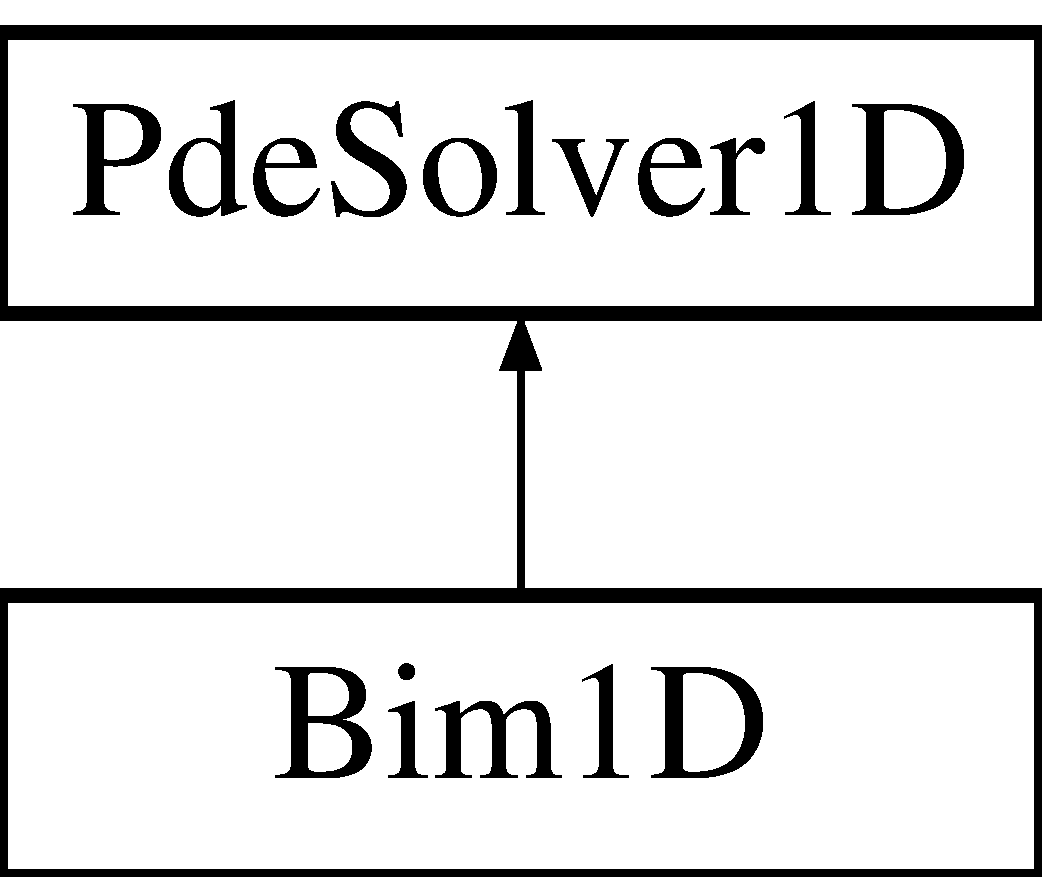
\includegraphics[height=2.000000cm]{classPdeSolver1D}
\end{center}
\end{figure}
\subsection*{Public Member Functions}
\begin{DoxyCompactItemize}
\item 
\hypertarget{classPdeSolver1D_a9e578d43e38517bade5c0911b7906e73}{\hyperlink{classPdeSolver1D_a9e578d43e38517bade5c0911b7906e73}{Pde\-Solver1\-D} ()=delete}\label{classPdeSolver1D_a9e578d43e38517bade5c0911b7906e73}

\begin{DoxyCompactList}\small\item\em Default constructor (deleted since it is required to specify the mesh). \end{DoxyCompactList}\item 
\hyperlink{classPdeSolver1D_a2fb4efbf180a22aa8d8404765a3a7aa5}{Pde\-Solver1\-D} (Vector\-Xd \&)
\begin{DoxyCompactList}\small\item\em Constructor. \end{DoxyCompactList}\item 
\hypertarget{classPdeSolver1D_ae52bcba084b9cc8daa575e3f06d9271a}{virtual \hyperlink{classPdeSolver1D_ae52bcba084b9cc8daa575e3f06d9271a}{$\sim$\-Pde\-Solver1\-D} ()=default}\label{classPdeSolver1D_ae52bcba084b9cc8daa575e3f06d9271a}

\begin{DoxyCompactList}\small\item\em Destructor (defaulted). \end{DoxyCompactList}\item 
virtual void \hyperlink{classPdeSolver1D_aa325f9e11f8b91cb22afca860888300d}{assemble\-Adv\-Diff} (const Vector\-Xd \&alpha, const Vector\-Xd \&gamma, const Vector\-Xd \&eta, const Vector\-Xd \&beta)=0
\begin{DoxyCompactList}\small\item\em Assemble the matrix for an advection-\/diffusion term. \end{DoxyCompactList}\item 
virtual void \hyperlink{classPdeSolver1D_af75110b5d68e91b62cfc3e7e4e969a32}{assemble\-Stiff} (const Vector\-Xd \&eps, const Vector\-Xd \&kappa)=0
\begin{DoxyCompactList}\small\item\em Assemble the matrix for a diffusion term. \end{DoxyCompactList}\item 
virtual void \hyperlink{classPdeSolver1D_aca065bfba5136470a4caf30fd7927e37}{assemble\-Mass} (const Vector\-Xd \&delta, const Vector\-Xd \&zeta)=0
\begin{DoxyCompactList}\small\item\em Assemble the matrix for a reaction term. \end{DoxyCompactList}\end{DoxyCompactItemize}
\begin{Indent}{\bf Getter methods.}\par
\begin{DoxyCompactItemize}
\item 
\hypertarget{classPdeSolver1D_a30abfde92c6d3c03a976287e968ed310}{const \hyperlink{typedefs_8h_a86edf437f454f4dd79d5422366403b7f}{Sparse\-Xd} \& {\bfseries Adv\-Diff} () const }\label{classPdeSolver1D_a30abfde92c6d3c03a976287e968ed310}

\item 
\hypertarget{classPdeSolver1D_ae27e38d5d2568ffdac3d4fd6b8399386}{const \hyperlink{typedefs_8h_a86edf437f454f4dd79d5422366403b7f}{Sparse\-Xd} \& {\bfseries Stiff} () const }\label{classPdeSolver1D_ae27e38d5d2568ffdac3d4fd6b8399386}

\item 
\hypertarget{classPdeSolver1D_ad68939b3aa2acb790cd4df84ea80b931}{const \hyperlink{typedefs_8h_a86edf437f454f4dd79d5422366403b7f}{Sparse\-Xd} \& {\bfseries Mass} () const }\label{classPdeSolver1D_ad68939b3aa2acb790cd4df84ea80b931}

\end{DoxyCompactItemize}
\end{Indent}
\subsection*{Protected Attributes}
\begin{DoxyCompactItemize}
\item 
\hypertarget{classPdeSolver1D_ac0185cf9f8cdf64273950a48d63df3f7}{Vector\-Xd \hyperlink{classPdeSolver1D_ac0185cf9f8cdf64273950a48d63df3f7}{mesh\-\_\-}}\label{classPdeSolver1D_ac0185cf9f8cdf64273950a48d63df3f7}

\begin{DoxyCompactList}\small\item\em The mesh. \end{DoxyCompactList}\item 
\hypertarget{classPdeSolver1D_a8f4bb43717322579edc12974700aec98}{unsigned \hyperlink{classPdeSolver1D_a8f4bb43717322579edc12974700aec98}{n\-Nodes\-\_\-}}\label{classPdeSolver1D_a8f4bb43717322579edc12974700aec98}

\begin{DoxyCompactList}\small\item\em No. of nodes that form the mesh. \end{DoxyCompactList}\item 
\hypertarget{classPdeSolver1D_a2febd884c8758db9fd346a40d81671eb}{\hyperlink{typedefs_8h_a86edf437f454f4dd79d5422366403b7f}{Sparse\-Xd} \hyperlink{classPdeSolver1D_a2febd884c8758db9fd346a40d81671eb}{Adv\-Diff\-\_\-}}\label{classPdeSolver1D_a2febd884c8758db9fd346a40d81671eb}

\begin{DoxyCompactList}\small\item\em Matrix for an advection-\/diffusion term. \end{DoxyCompactList}\item 
\hypertarget{classPdeSolver1D_a63de5de1757c8bc5cd0941030f9794e3}{\hyperlink{typedefs_8h_a86edf437f454f4dd79d5422366403b7f}{Sparse\-Xd} \hyperlink{classPdeSolver1D_a63de5de1757c8bc5cd0941030f9794e3}{Stiff\-\_\-}}\label{classPdeSolver1D_a63de5de1757c8bc5cd0941030f9794e3}

\begin{DoxyCompactList}\small\item\em Stiffness matrix. \end{DoxyCompactList}\item 
\hypertarget{classPdeSolver1D_aa0e70aa868721f4bbf1fe7ec57e097a9}{\hyperlink{typedefs_8h_a86edf437f454f4dd79d5422366403b7f}{Sparse\-Xd} \hyperlink{classPdeSolver1D_aa0e70aa868721f4bbf1fe7ec57e097a9}{Mass\-\_\-}}\label{classPdeSolver1D_aa0e70aa868721f4bbf1fe7ec57e097a9}

\begin{DoxyCompactList}\small\item\em Mass matrix. \end{DoxyCompactList}\end{DoxyCompactItemize}
\subsection*{Friends}
\begin{DoxyCompactItemize}
\item 
\hypertarget{classPdeSolver1D_a77f1c8533ec7e07072fed14bad6ae1a8}{class {\bfseries Non\-Linear\-Poisson1\-D}}\label{classPdeSolver1D_a77f1c8533ec7e07072fed14bad6ae1a8}

\end{DoxyCompactItemize}


\subsection{Detailed Description}
Abstract class providing methods to assemble matrices to solve one-\/dimensional P\-D\-Es. 

Matrices are held in a sparse format. 

\subsection{Constructor \& Destructor Documentation}
\hypertarget{classPdeSolver1D_a2fb4efbf180a22aa8d8404765a3a7aa5}{\index{Pde\-Solver1\-D@{Pde\-Solver1\-D}!Pde\-Solver1\-D@{Pde\-Solver1\-D}}
\index{Pde\-Solver1\-D@{Pde\-Solver1\-D}!PdeSolver1D@{Pde\-Solver1\-D}}
\subsubsection[{Pde\-Solver1\-D}]{\setlength{\rightskip}{0pt plus 5cm}{\bf Pde\-Solver1\-D} (
\begin{DoxyParamCaption}
\item[{Vector\-Xd \&}]{mesh}
\end{DoxyParamCaption}
)}}\label{classPdeSolver1D_a2fb4efbf180a22aa8d8404765a3a7aa5}


Constructor. 


\begin{DoxyParams}[1]{Parameters}
\mbox{\tt in}  & {\em mesh} & \-: the mesh. \\
\hline
\end{DoxyParams}


\subsection{Member Function Documentation}
\hypertarget{classPdeSolver1D_aa325f9e11f8b91cb22afca860888300d}{\index{Pde\-Solver1\-D@{Pde\-Solver1\-D}!assemble\-Adv\-Diff@{assemble\-Adv\-Diff}}
\index{assemble\-Adv\-Diff@{assemble\-Adv\-Diff}!PdeSolver1D@{Pde\-Solver1\-D}}
\subsubsection[{assemble\-Adv\-Diff}]{\setlength{\rightskip}{0pt plus 5cm}virtual void assemble\-Adv\-Diff (
\begin{DoxyParamCaption}
\item[{const Vector\-Xd \&}]{alpha, }
\item[{const Vector\-Xd \&}]{gamma, }
\item[{const Vector\-Xd \&}]{eta, }
\item[{const Vector\-Xd \&}]{beta}
\end{DoxyParamCaption}
)\hspace{0.3cm}{\ttfamily [pure virtual]}}}\label{classPdeSolver1D_aa325f9e11f8b91cb22afca860888300d}


Assemble the matrix for an advection-\/diffusion term. 

Build the matrix for the advection-\/diffusion problem\-: $ -\nabla\cdot\left(\alpha\cdot\gamma\left(\eta\nabla u - \beta u\right)\right) = f $.


\begin{DoxyParams}[1]{Parameters}
\mbox{\tt in}  & {\em alpha} & \-: $ \alpha $, an element-\/wise constant function; \\
\hline
\mbox{\tt in}  & {\em gamma} & \-: $ \gamma $, an element-\/wise linear function; \\
\hline
\mbox{\tt in}  & {\em eta} & \-: $ \eta $, an element-\/wise linear function; \\
\hline
\mbox{\tt in}  & {\em beta} & \-: $ \beta $, an element-\/wise constant function. \\
\hline
\end{DoxyParams}


Implemented in \hyperlink{classBim1D_a70f740fd42f21c2284f4c67c94b36ef3}{Bim1\-D}.

\hypertarget{classPdeSolver1D_af75110b5d68e91b62cfc3e7e4e969a32}{\index{Pde\-Solver1\-D@{Pde\-Solver1\-D}!assemble\-Stiff@{assemble\-Stiff}}
\index{assemble\-Stiff@{assemble\-Stiff}!PdeSolver1D@{Pde\-Solver1\-D}}
\subsubsection[{assemble\-Stiff}]{\setlength{\rightskip}{0pt plus 5cm}virtual void assemble\-Stiff (
\begin{DoxyParamCaption}
\item[{const Vector\-Xd \&}]{eps, }
\item[{const Vector\-Xd \&}]{kappa}
\end{DoxyParamCaption}
)\hspace{0.3cm}{\ttfamily [pure virtual]}}}\label{classPdeSolver1D_af75110b5d68e91b62cfc3e7e4e969a32}


Assemble the matrix for a diffusion term. 

Build the matrix for the diffusion problem\-: $ -\nabla\cdot\left(\epsilon\cdot\kappa\nabla u\right) = f $.


\begin{DoxyParams}[1]{Parameters}
\mbox{\tt in}  & {\em eps} & \-: $ \epsilon $, an element-\/wise constant function; \\
\hline
\mbox{\tt in}  & {\em kappa} & \-: $ \kappa $, an element-\/wise linear function. \\
\hline
\end{DoxyParams}


Implemented in \hyperlink{classBim1D_ad16a59cddd56a41185163574507dfdef}{Bim1\-D}.

\hypertarget{classPdeSolver1D_aca065bfba5136470a4caf30fd7927e37}{\index{Pde\-Solver1\-D@{Pde\-Solver1\-D}!assemble\-Mass@{assemble\-Mass}}
\index{assemble\-Mass@{assemble\-Mass}!PdeSolver1D@{Pde\-Solver1\-D}}
\subsubsection[{assemble\-Mass}]{\setlength{\rightskip}{0pt plus 5cm}virtual void assemble\-Mass (
\begin{DoxyParamCaption}
\item[{const Vector\-Xd \&}]{delta, }
\item[{const Vector\-Xd \&}]{zeta}
\end{DoxyParamCaption}
)\hspace{0.3cm}{\ttfamily [pure virtual]}}}\label{classPdeSolver1D_aca065bfba5136470a4caf30fd7927e37}


Assemble the matrix for a reaction term. 

Build the mass matrix for the reaction problem\-: $ \delta\cdot\zeta u = f $.


\begin{DoxyParams}[1]{Parameters}
\mbox{\tt in}  & {\em delta} & \-: $ \delta $, an element-\/wise constant function; \\
\hline
\mbox{\tt in}  & {\em zeta} & \-: $ \zeta $, an element-\/wise linear function. \\
\hline
\end{DoxyParams}


Implemented in \hyperlink{classBim1D_aa99f58d5ec1d53891b11ea81adec6b92}{Bim1\-D}.



The documentation for this class was generated from the following files\-:\begin{DoxyCompactItemize}
\item 
/home/\-Data/\-Dropbox/\-Progetto-\/\-P\-A\-C\-S/\-C++/\-Source/src/\hyperlink{solvers_8h}{solvers.\-h}\item 
/home/\-Data/\-Dropbox/\-Progetto-\/\-P\-A\-C\-S/\-C++/\-Source/src/solvers.\-c++\end{DoxyCompactItemize}

\hypertarget{classQuadratureRule}{\section{Quadrature\-Rule Class Reference}
\label{classQuadratureRule}\index{Quadrature\-Rule@{Quadrature\-Rule}}
}


Abstract class providing a quadrature rule.  




{\ttfamily \#include $<$quadrature\-Rule.\-h$>$}

Inheritance diagram for Quadrature\-Rule\-:\begin{figure}[H]
\begin{center}
\leavevmode
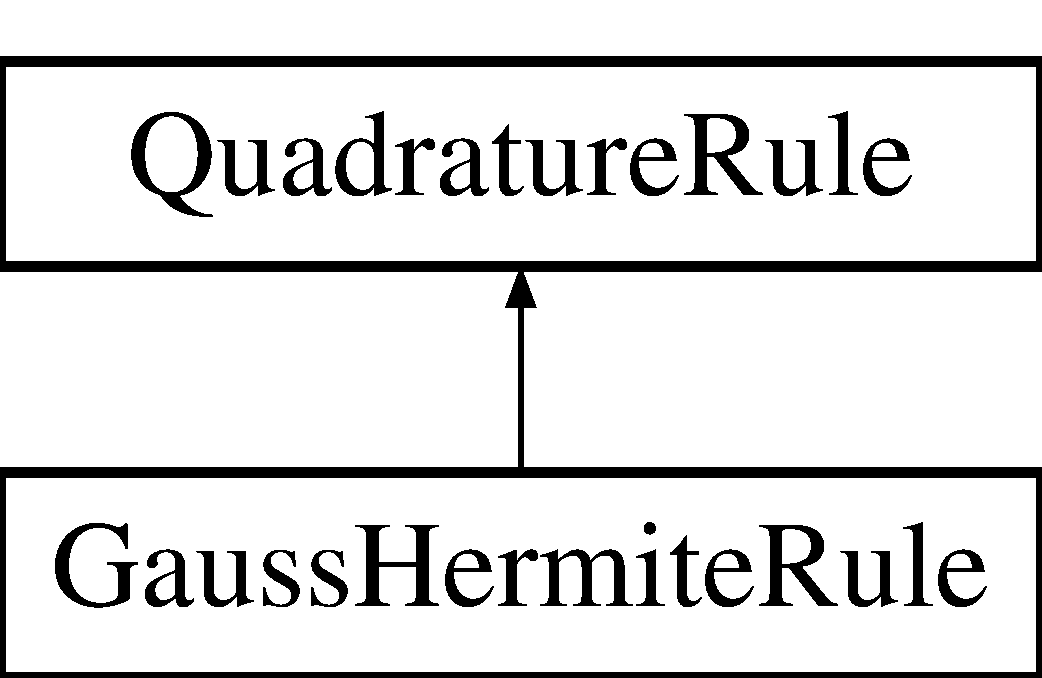
\includegraphics[height=2.000000cm]{classQuadratureRule}
\end{center}
\end{figure}
\subsection*{Public Member Functions}
\begin{DoxyCompactItemize}
\item 
\hypertarget{classQuadratureRule_ac7fb9aaf8e3f9eae03235f68a935880a}{\hyperlink{classQuadratureRule_ac7fb9aaf8e3f9eae03235f68a935880a}{Quadrature\-Rule} ()=delete}\label{classQuadratureRule_ac7fb9aaf8e3f9eae03235f68a935880a}

\begin{DoxyCompactList}\small\item\em Default constructor (deleted since it is required to specify the number of nodes). \end{DoxyCompactList}\item 
\hyperlink{classQuadratureRule_a1d658803a64ae7aa2d9a59754483f8a0}{Quadrature\-Rule} (const \hyperlink{typedefs_8h_a2c726f8f32697958e9d6c2afecda531d}{Index} \&)
\begin{DoxyCompactList}\small\item\em Constructor. \end{DoxyCompactList}\item 
\hypertarget{classQuadratureRule_a80e11fbb08b332f2d4c56740cb63ac4e}{virtual \hyperlink{classQuadratureRule_a80e11fbb08b332f2d4c56740cb63ac4e}{$\sim$\-Quadrature\-Rule} ()=default}\label{classQuadratureRule_a80e11fbb08b332f2d4c56740cb63ac4e}

\begin{DoxyCompactList}\small\item\em Destructor (defaulted). \end{DoxyCompactList}\item 
\hypertarget{classQuadratureRule_ae8035f1283a63c55fbbfb4e786db8a98}{virtual void \hyperlink{classQuadratureRule_ae8035f1283a63c55fbbfb4e786db8a98}{apply} ()=0}\label{classQuadratureRule_ae8035f1283a63c55fbbfb4e786db8a98}

\begin{DoxyCompactList}\small\item\em Apply the quadrature rule in order to compute the nodes and weights. \end{DoxyCompactList}\end{DoxyCompactItemize}
\begin{Indent}{\bf Getter methods}\par
\begin{DoxyCompactItemize}
\item 
\hypertarget{classQuadratureRule_a32e8457e19f3f8f4096e82a0cd759a03}{const \hyperlink{typedefs_8h_a2c726f8f32697958e9d6c2afecda531d}{Index} \& {\bfseries n\-Nodes} () const }\label{classQuadratureRule_a32e8457e19f3f8f4096e82a0cd759a03}

\item 
\hypertarget{classQuadratureRule_ac955b3953fe9174d6c9c4c9f519b4858}{const \hyperlink{typedefs_8h_aae6cee78ed9cd8f234ed8cb48682548a}{Vector\-Xr} \& {\bfseries nodes} () const }\label{classQuadratureRule_ac955b3953fe9174d6c9c4c9f519b4858}

\item 
\hypertarget{classQuadratureRule_a34502030990595ad6c2ededfb52383ae}{const \hyperlink{typedefs_8h_aae6cee78ed9cd8f234ed8cb48682548a}{Vector\-Xr} \& {\bfseries weights} () const }\label{classQuadratureRule_a34502030990595ad6c2ededfb52383ae}

\end{DoxyCompactItemize}
\end{Indent}
\subsection*{Protected Attributes}
\begin{DoxyCompactItemize}
\item 
\hypertarget{classQuadratureRule_a574676917a0d7d70140f4ed29bb1e8b4}{\hyperlink{typedefs_8h_a2c726f8f32697958e9d6c2afecda531d}{Index} \hyperlink{classQuadratureRule_a574676917a0d7d70140f4ed29bb1e8b4}{n\-Nodes\-\_\-}}\label{classQuadratureRule_a574676917a0d7d70140f4ed29bb1e8b4}

\begin{DoxyCompactList}\small\item\em Number of nodes of quadrature. \end{DoxyCompactList}\item 
\hypertarget{classQuadratureRule_af96d558adb075a6049017281e98fbed3}{\hyperlink{typedefs_8h_aae6cee78ed9cd8f234ed8cb48682548a}{Vector\-Xr} \hyperlink{classQuadratureRule_af96d558adb075a6049017281e98fbed3}{nodes\-\_\-}}\label{classQuadratureRule_af96d558adb075a6049017281e98fbed3}

\begin{DoxyCompactList}\small\item\em Vector containing the computed nodes coordinates. \end{DoxyCompactList}\item 
\hypertarget{classQuadratureRule_a35b6b677135284647f99765144b3af7a}{\hyperlink{typedefs_8h_aae6cee78ed9cd8f234ed8cb48682548a}{Vector\-Xr} \hyperlink{classQuadratureRule_a35b6b677135284647f99765144b3af7a}{weights\-\_\-}}\label{classQuadratureRule_a35b6b677135284647f99765144b3af7a}

\begin{DoxyCompactList}\small\item\em Vector containing the computed weights. \end{DoxyCompactList}\end{DoxyCompactItemize}
\subsection*{Friends}
\begin{DoxyCompactItemize}
\item 
\hypertarget{classQuadratureRule_a6be33a81953be5c0377a00dec7d5b1d3}{class {\bfseries Gaussian\-Charge}}\label{classQuadratureRule_a6be33a81953be5c0377a00dec7d5b1d3}

\end{DoxyCompactItemize}


\subsection{Detailed Description}
Abstract class providing a quadrature rule. 

Approximate the integral\-: \[ \int_{a}^{b} f(x)~\mathrm{d}x \] with the finite sum\-: \[ \sum_{i=1}^{nNodes\_} w_i \cdot f(x_i) \] where $ \{x_i\}_{i=1}^{nNodes\_} $ and $ \{w_i\}_{i=1}^{nNodes\_} $ are called respectively nodes and weights. 

Definition at line 29 of file quadrature\-Rule.\-h.



\subsection{Constructor \& Destructor Documentation}
\hypertarget{classQuadratureRule_a1d658803a64ae7aa2d9a59754483f8a0}{\index{Quadrature\-Rule@{Quadrature\-Rule}!Quadrature\-Rule@{Quadrature\-Rule}}
\index{Quadrature\-Rule@{Quadrature\-Rule}!QuadratureRule@{Quadrature\-Rule}}
\subsubsection[{Quadrature\-Rule}]{\setlength{\rightskip}{0pt plus 5cm}{\bf Quadrature\-Rule} (
\begin{DoxyParamCaption}
\item[{const {\bf Index} \&}]{n\-Nodes}
\end{DoxyParamCaption}
)}}\label{classQuadratureRule_a1d658803a64ae7aa2d9a59754483f8a0}


Constructor. 


\begin{DoxyParams}[1]{Parameters}
\mbox{\tt in}  & {\em n\-Nodes} & \-: the number of nodes to be used for the quadrature rule. \\
\hline
\end{DoxyParams}


Definition at line 5 of file quadrature\-Rule.\-c++.



The documentation for this class was generated from the following files\-:\begin{DoxyCompactItemize}
\item 
/home/elauksap/\-Dropbox/\-Progetto-\/\-P\-A\-C\-S/\-C++/\-Source/src/\hyperlink{quadratureRule_8h}{quadrature\-Rule.\-h}\item 
/home/elauksap/\-Dropbox/\-Progetto-\/\-P\-A\-C\-S/\-C++/\-Source/src/quadrature\-Rule.\-c++\end{DoxyCompactItemize}

\chapter{File Documentation}
\hypertarget{simulate__dos_8c_09_09}{\section{/home/elauksap/\-Dropbox/\-Progetto-\/\-P\-A\-C\-S/\-C++/\-Source/test/simulate\-\_\-dos.c++ File Reference}
\label{simulate__dos_8c_09_09}\index{/home/elauksap/\-Dropbox/\-Progetto-\/\-P\-A\-C\-S/\-C++/\-Source/test/simulate\-\_\-dos.\-c++@{/home/elauksap/\-Dropbox/\-Progetto-\/\-P\-A\-C\-S/\-C++/\-Source/test/simulate\-\_\-dos.\-c++}}
}


A test file.  


{\ttfamily \#include \char`\"{}src/dos\-Model.\-h\char`\"{}}\\*
\subsection*{Functions}
\begin{DoxyCompactItemize}
\item 
\hypertarget{simulate__dos_8c_09_09_abb42499d73e7c21855b75ac125b8da84}{int \hyperlink{simulate__dos_8c_09_09_abb42499d73e7c21855b75ac125b8da84}{main} (const int argc, const char $\ast$const $\ast$argv, const char $\ast$const $\ast$envp)}\label{simulate__dos_8c_09_09_abb42499d73e7c21855b75ac125b8da84}

\begin{DoxyCompactList}\small\item\em The {\bfseries main} function. \end{DoxyCompactList}\end{DoxyCompactItemize}


\subsection{Detailed Description}
A test file. \begin{DoxyAuthor}{Author}
Pasquale Claudio Africa \href{mailto:pasquale.africa@gmail.com}{\tt pasquale.\-africa@gmail.\-com} 
\end{DoxyAuthor}
\begin{DoxyDate}{Date}
2014 
\end{DoxyDate}


Definition in file \hyperlink{simulate__dos_8c_09_09_source}{simulate\-\_\-dos.\-c++}.


\hypertarget{charge_8h}{\section{/home/elauksap/\-Dropbox/\-Progetto-\/\-P\-A\-C\-S/\-C++/\-Source/src/charge.h File Reference}
\label{charge_8h}\index{/home/elauksap/\-Dropbox/\-Progetto-\/\-P\-A\-C\-S/\-C++/\-Source/src/charge.\-h@{/home/elauksap/\-Dropbox/\-Progetto-\/\-P\-A\-C\-S/\-C++/\-Source/src/charge.\-h}}
}


Classes for computing total electric charge.  


{\ttfamily \#include \char`\"{}param\-List.\-h\char`\"{}}\\*
{\ttfamily \#include \char`\"{}quadrature\-Rule.\-h\char`\"{}}\\*
{\ttfamily \#include \char`\"{}typedefs.\-h\char`\"{}}\\*
\subsection*{Classes}
\begin{DoxyCompactItemize}
\item 
class \hyperlink{classCharge}{Charge}
\begin{DoxyCompactList}\small\item\em Abstract class providing methods to calculate total electric charge (the rhs in the Poisson equation). \end{DoxyCompactList}\item 
class \hyperlink{classGaussianCharge}{Gaussian\-Charge}
\begin{DoxyCompactList}\small\item\em Class derived from \hyperlink{classCharge}{Charge}, under the hypothesis that Density of States is a combination of gaussians. \end{DoxyCompactList}\item 
class \hyperlink{classExponentialCharge}{Exponential\-Charge}
\begin{DoxyCompactList}\small\item\em Class derived from \hyperlink{classCharge}{Charge}, under the hypothesis that Density of States is a single exponential. \end{DoxyCompactList}\end{DoxyCompactItemize}


\subsection{Detailed Description}
Classes for computing total electric charge. \begin{DoxyAuthor}{Author}
Pasquale Claudio Africa \href{mailto:pasquale.africa@gmail.com}{\tt pasquale.\-africa@gmail.\-com} 
\end{DoxyAuthor}
\begin{DoxyDate}{Date}
2014
\end{DoxyDate}
\begin{DoxyCopyright}{Copyright}
Copyright © 2014 Pasquale Claudio Africa. All rights reserved. 

This project is released under the G\-N\-U General Public License. 
\end{DoxyCopyright}


Definition in file \hyperlink{charge_8h_source}{charge.\-h}.


\hypertarget{csvParser_8h}{\section{/home/elauksap/\-Dropbox/\-Progetto-\/\-P\-A\-C\-S/\-C++/\-Source/src/csv\-Parser.h File Reference}
\label{csvParser_8h}\index{/home/elauksap/\-Dropbox/\-Progetto-\/\-P\-A\-C\-S/\-C++/\-Source/src/csv\-Parser.\-h@{/home/elauksap/\-Dropbox/\-Progetto-\/\-P\-A\-C\-S/\-C++/\-Source/src/csv\-Parser.\-h}}
}


Tools to store content from a .csv file in matrices or vectors.  


{\ttfamily \#include \char`\"{}typedefs.\-h\char`\"{}}\\*
{\ttfamily \#include $<$string$>$}\\*
{\ttfamily \#include $<$fstream$>$}\\*
{\ttfamily \#include $<$sstream$>$}\\*
{\ttfamily \#include $<$utility$>$}\\*
\subsection*{Classes}
\begin{DoxyCompactItemize}
\item 
class \hyperlink{classCsvParser}{Csv\-Parser}
\begin{DoxyCompactList}\small\item\em Class providing methods to read {\bfseries numeric} content from a .csv file and to store it in \hyperlink{index_Eigen}{Eigen} matrices or vectors. \end{DoxyCompactList}\end{DoxyCompactItemize}


\subsection{Detailed Description}
Tools to store content from a .csv file in matrices or vectors. \begin{DoxyAuthor}{Author}
Pasquale Claudio Africa \href{mailto:pasquale.africa@gmail.com}{\tt pasquale.\-africa@gmail.\-com} 
\end{DoxyAuthor}
\begin{DoxyDate}{Date}
2014
\end{DoxyDate}
\begin{DoxyCopyright}{Copyright}
Copyright © 2014 Pasquale Claudio Africa. All rights reserved. 

This project is released under the G\-N\-U General Public License. 
\end{DoxyCopyright}


Definition in file \hyperlink{csvParser_8h_source}{csv\-Parser.\-h}.


\hypertarget{dosModel_8h}{\section{/home/elauksap/\-Dropbox/\-Progetto-\/\-P\-A\-C\-S/\-C++/\-Source/src/dos\-Model.h File Reference}
\label{dosModel_8h}\index{/home/elauksap/\-Dropbox/\-Progetto-\/\-P\-A\-C\-S/\-C++/\-Source/src/dos\-Model.\-h@{/home/elauksap/\-Dropbox/\-Progetto-\/\-P\-A\-C\-S/\-C++/\-Source/src/dos\-Model.\-h}}
}


Mathematical model for Density of States extraction.  


{\ttfamily \#include \char`\"{}charge.\-h\char`\"{}}\\*
{\ttfamily \#include \char`\"{}csv\-Parser.\-h\char`\"{}}\\*
{\ttfamily \#include \char`\"{}factory.\-h\char`\"{}}\\*
{\ttfamily \#include \char`\"{}numerics.\-h\char`\"{}}\\*
{\ttfamily \#include \char`\"{}param\-List.\-h\char`\"{}}\\*
{\ttfamily \#include \char`\"{}quadrature\-Rule.\-h\char`\"{}}\\*
{\ttfamily \#include \char`\"{}solvers.\-h\char`\"{}}\\*
{\ttfamily \#include \char`\"{}typedefs.\-h\char`\"{}}\\*
{\ttfamily \#include \char`\"{}gnuplot-\/iostream.\-h\char`\"{}}\\*
{\ttfamily \#include $<$chrono$>$}\\*
{\ttfamily \#include $<$limits$>$}\\*
\subsection*{Classes}
\begin{DoxyCompactItemize}
\item 
class \hyperlink{classDosModel}{Dos\-Model}
\begin{DoxyCompactList}\small\item\em Class providing methods to process a simulation to extract the Density of States starting from a parameter list. \end{DoxyCompactList}\end{DoxyCompactItemize}


\subsection{Detailed Description}
Mathematical model for Density of States extraction. \begin{DoxyAuthor}{Author}
Pasquale Claudio Africa \href{mailto:pasquale.africa@gmail.com}{\tt pasquale.\-africa@gmail.\-com} 
\end{DoxyAuthor}
\begin{DoxyDate}{Date}
2014
\end{DoxyDate}
\begin{DoxyCopyright}{Copyright}
Copyright © 2014 Pasquale Claudio Africa. All rights reserved. 

This project is released under the G\-N\-U General Public License. 
\end{DoxyCopyright}


Definition in file \hyperlink{dosModel_8h_source}{dos\-Model.\-h}.


\hypertarget{numerics_8h}{\section{/home/\-Data/\-Dropbox/\-Progetto-\/\-P\-A\-C\-S/\-C++/\-Source/src/numerics.h File Reference}
\label{numerics_8h}\index{/home/\-Data/\-Dropbox/\-Progetto-\/\-P\-A\-C\-S/\-C++/\-Source/src/numerics.\-h@{/home/\-Data/\-Dropbox/\-Progetto-\/\-P\-A\-C\-S/\-C++/\-Source/src/numerics.\-h}}
}


Generic numeric algorithms.  


{\ttfamily \#include \char`\"{}typedefs.\-h\char`\"{}}\\*
{\ttfamily \#include $<$limits$>$}\\*
\subsection*{Namespaces}
\begin{DoxyCompactItemize}
\item 
\hyperlink{namespacenumerics}{numerics}
\begin{DoxyCompactList}\small\item\em Namespace for generic numeric algorithms. \end{DoxyCompactList}\end{DoxyCompactItemize}
\subsection*{Functions}
\begin{DoxyCompactItemize}
\item 
{\footnotesize template$<$typename Scalar\-Type $>$ }\\\hyperlink{typedefs_8h_ac264e7346c0c88c8a573518d1e8f8c3d}{Vector\-X}$<$ Scalar\-Type $>$ \hyperlink{namespacenumerics_a1633aabded7159bb15bbf573bf9e12c5}{sort} (const \hyperlink{typedefs_8h_ac264e7346c0c88c8a573518d1e8f8c3d}{Vector\-X}$<$ Scalar\-Type $>$ \&vector)
\begin{DoxyCompactList}\small\item\em Function to sort \hyperlink{index_Eigen}{Eigen} vectors. \end{DoxyCompactList}\item 
{\footnotesize template$<$typename Scalar\-Type $>$ }\\\hyperlink{typedefs_8h_af38b14e4434227fa8e1b41e0d6632171}{Vector\-Xpair}$<$ Scalar\-Type $>$ \hyperlink{namespacenumerics_a510fe73118ce8c79570ac87fa3e7df47}{sort\-\_\-pair} (const \hyperlink{typedefs_8h_ac264e7346c0c88c8a573518d1e8f8c3d}{Vector\-X}$<$ Scalar\-Type $>$ \&vector)
\begin{DoxyCompactList}\small\item\em Function to sort \hyperlink{index_Eigen}{Eigen} vectors, keeping track of indexes. \end{DoxyCompactList}\item 
\hyperlink{typedefs_8h_a060b837c3b4486ee35317744156f3da2}{Real} \hyperlink{namespacenumerics_a41daad9dd743c914a195298bda0c0269}{trapz} (const \hyperlink{typedefs_8h_aae6cee78ed9cd8f234ed8cb48682548a}{Vector\-Xr} \&x, const \hyperlink{typedefs_8h_aae6cee78ed9cd8f234ed8cb48682548a}{Vector\-Xr} \&y)
\begin{DoxyCompactList}\small\item\em Function to compute approximate integral of {\itshape y} with spacing increment specified by {\itshape x}, using trapezoidal rule. \end{DoxyCompactList}\item 
\hyperlink{typedefs_8h_a060b837c3b4486ee35317744156f3da2}{Real} \hyperlink{namespacenumerics_a24c140740098eaaa477d8ec263fbb441}{trapz} (const \hyperlink{typedefs_8h_aae6cee78ed9cd8f234ed8cb48682548a}{Vector\-Xr} \&y)
\begin{DoxyCompactList}\small\item\em Compute the approximate integral of {\itshape y} with unit spacing, using trapezoidal rule. \end{DoxyCompactList}\item 
\hyperlink{typedefs_8h_aae6cee78ed9cd8f234ed8cb48682548a}{Vector\-Xr} \hyperlink{namespacenumerics_a8ba4a40c596ac41f1438a34c1e91d19d}{deriv} (const \hyperlink{typedefs_8h_aae6cee78ed9cd8f234ed8cb48682548a}{Vector\-Xr} \&, const \hyperlink{typedefs_8h_aae6cee78ed9cd8f234ed8cb48682548a}{Vector\-Xr} \&)
\begin{DoxyCompactList}\small\item\em Compute the numeric derivative\-: $ \frac{\mathrm{d}y}{\mathrm{d}x} $. \end{DoxyCompactList}\item 
\hyperlink{typedefs_8h_a060b837c3b4486ee35317744156f3da2}{Real} \hyperlink{namespacenumerics_a05cd7efecfbd0a2771993848352e2e2d}{interp1} (const \hyperlink{typedefs_8h_aae6cee78ed9cd8f234ed8cb48682548a}{Vector\-Xr} \&, const \hyperlink{typedefs_8h_aae6cee78ed9cd8f234ed8cb48682548a}{Vector\-Xr} \&, const \hyperlink{typedefs_8h_a060b837c3b4486ee35317744156f3da2}{Real} \&)
\begin{DoxyCompactList}\small\item\em Linear 1\-D interpolation. Interpolate {\itshape y}, defined at points {\itshape x}, at the point {\itshape x\-New}. \end{DoxyCompactList}\item 
\hyperlink{typedefs_8h_aae6cee78ed9cd8f234ed8cb48682548a}{Vector\-Xr} \hyperlink{namespacenumerics_a5056bae21df918a09efaf5fb45300bff}{interp1} (const \hyperlink{typedefs_8h_aae6cee78ed9cd8f234ed8cb48682548a}{Vector\-Xr} \&, const \hyperlink{typedefs_8h_aae6cee78ed9cd8f234ed8cb48682548a}{Vector\-Xr} \&, const \hyperlink{typedefs_8h_aae6cee78ed9cd8f234ed8cb48682548a}{Vector\-Xr} \&)
\begin{DoxyCompactList}\small\item\em Linear 1\-D interpolation. Interpolate {\itshape y}, defined at points {\itshape x}, at the points {\itshape x\-New}. \end{DoxyCompactList}\item 
\hyperlink{typedefs_8h_a060b837c3b4486ee35317744156f3da2}{Real} \hyperlink{namespacenumerics_a7beb6807c580a205d0c23b4a9b23213f}{error\-\_\-\-L2} (const \hyperlink{typedefs_8h_aae6cee78ed9cd8f234ed8cb48682548a}{Vector\-Xr} \&, const \hyperlink{typedefs_8h_aae6cee78ed9cd8f234ed8cb48682548a}{Vector\-Xr} \&, const \hyperlink{typedefs_8h_aae6cee78ed9cd8f234ed8cb48682548a}{Vector\-Xr} \&, const \hyperlink{typedefs_8h_a060b837c3b4486ee35317744156f3da2}{Real} \&)
\begin{DoxyCompactList}\small\item\em Compute the $ L^2 $-\/norm error between simulated and interpolated values, using {\itshape trapz}. \end{DoxyCompactList}\end{DoxyCompactItemize}


\subsection{Detailed Description}
Generic numeric algorithms. \begin{DoxyAuthor}{Author}
Pasquale Claudio Africa \href{mailto:pasquale.africa@gmail.com}{\tt pasquale.\-africa@gmail.\-com} 
\end{DoxyAuthor}
\begin{DoxyDate}{Date}
2014 
\end{DoxyDate}


Definition in file \hyperlink{numerics_8h_source}{numerics.\-h}.


\hypertarget{paramList_8h}{\section{/home/elauksap/\-Dropbox/\-Progetto-\/\-P\-A\-C\-S/\-C++/\-Source/src/param\-List.h File Reference}
\label{paramList_8h}\index{/home/elauksap/\-Dropbox/\-Progetto-\/\-P\-A\-C\-S/\-C++/\-Source/src/param\-List.\-h@{/home/elauksap/\-Dropbox/\-Progetto-\/\-P\-A\-C\-S/\-C++/\-Source/src/param\-List.\-h}}
}


List of simulation parameters.  


{\ttfamily \#include \char`\"{}typedefs.\-h\char`\"{}}\\*
\subsection*{Classes}
\begin{DoxyCompactItemize}
\item 
class \hyperlink{classParamList}{Param\-List}
\begin{DoxyCompactList}\small\item\em Class providing methods to handle a list of parameters. \end{DoxyCompactList}\end{DoxyCompactItemize}


\subsection{Detailed Description}
List of simulation parameters. \begin{DoxyAuthor}{Author}
Pasquale Claudio Africa \href{mailto:pasquale.africa@gmail.com}{\tt pasquale.\-africa@gmail.\-com} 
\end{DoxyAuthor}
\begin{DoxyDate}{Date}
2014
\end{DoxyDate}
\begin{DoxyCopyright}{Copyright}
Copyright © 2014 Pasquale Claudio Africa. All rights reserved. 

This project is released under the G\-N\-U General Public License. 
\end{DoxyCopyright}


Definition in file \hyperlink{paramList_8h_source}{param\-List.\-h}.


\hypertarget{physicalConstants_8h}{\section{Dos\-Extraction/src/physical\-Constants.h File Reference}
\label{physicalConstants_8h}\index{Dos\-Extraction/src/physical\-Constants.\-h@{Dos\-Extraction/src/physical\-Constants.\-h}}
}


Physical constants.  


This graph shows which files directly or indirectly include this file\-:\nopagebreak
\begin{figure}[H]
\begin{center}
\leavevmode
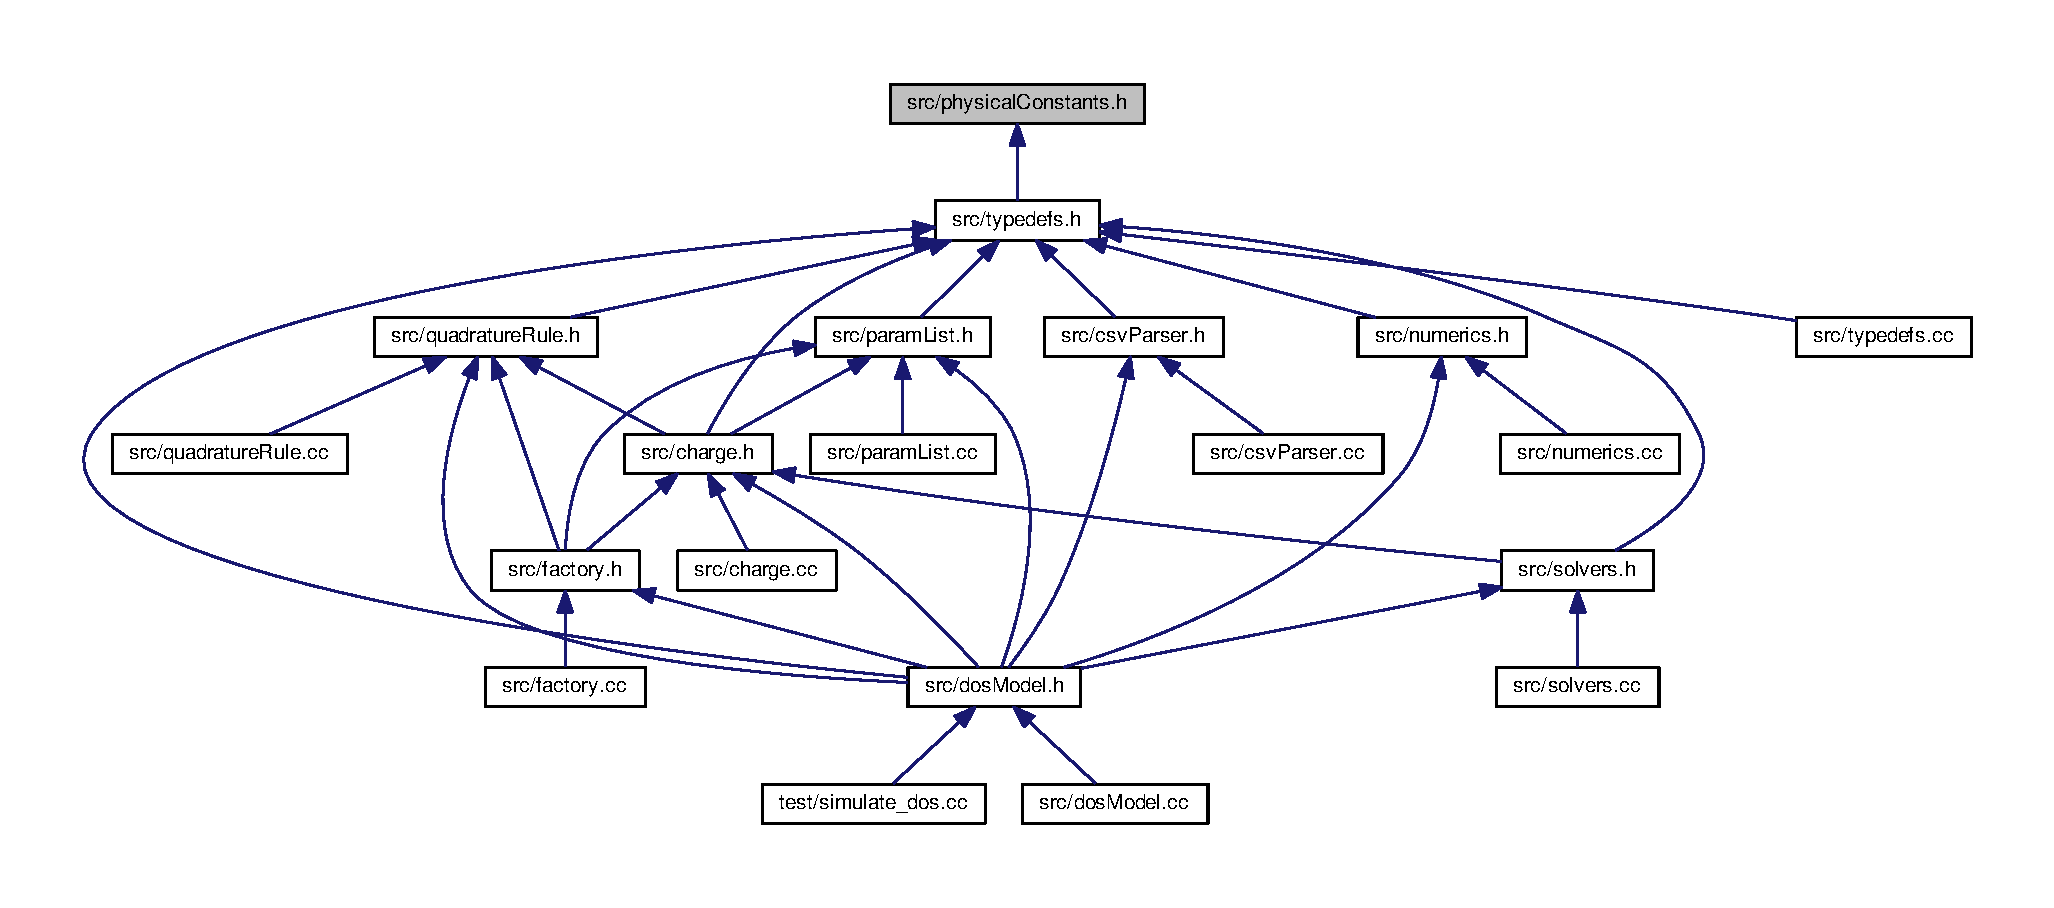
\includegraphics[width=350pt]{physicalConstants_8h__dep__incl}
\end{center}
\end{figure}
\subsection*{Namespaces}
\begin{DoxyCompactItemize}
\item 
\hyperlink{namespaceconstants}{constants}
\begin{DoxyCompactList}\small\item\em Numerical constants. \end{DoxyCompactList}\end{DoxyCompactItemize}
\subsection*{Variables}
\begin{DoxyCompactItemize}
\item 
\hypertarget{namespaceconstants_a791181f54af6cd7794fe58fec8e4ce97}{const \hyperlink{typedefs_8h_a060b837c3b4486ee35317744156f3da2}{Real} \hyperlink{namespaceconstants_a791181f54af6cd7794fe58fec8e4ce97}{Q} = 1.\-60217653000000e-\/19}\label{namespaceconstants_a791181f54af6cd7794fe58fec8e4ce97}

\begin{DoxyCompactList}\small\item\em Electron charge $ \left[ C \right] $. \end{DoxyCompactList}\item 
\hypertarget{namespaceconstants_a6af60c0507d9627b476d85e3275b161e}{const \hyperlink{typedefs_8h_a060b837c3b4486ee35317744156f3da2}{Real} \hyperlink{namespaceconstants_a6af60c0507d9627b476d85e3275b161e}{Q2} = Q $\ast$ Q}\label{namespaceconstants_a6af60c0507d9627b476d85e3275b161e}

\begin{DoxyCompactList}\small\item\em Electron charge squared $ \left[ C^2 \right] $. \end{DoxyCompactList}\item 
\hypertarget{namespaceconstants_a02b04d1da9b8254ea609a8334de09da7}{const \hyperlink{typedefs_8h_a060b837c3b4486ee35317744156f3da2}{Real} \hyperlink{namespaceconstants_a02b04d1da9b8254ea609a8334de09da7}{K\-\_\-\-B} = 1.\-38065050000000e-\/23}\label{namespaceconstants_a02b04d1da9b8254ea609a8334de09da7}

\begin{DoxyCompactList}\small\item\em Boltzmann's constant $ \left[ J \cdot K^{-1} \right] $. \end{DoxyCompactList}\item 
\hypertarget{namespaceconstants_a1be297a9c9ca81f310b848dbe6c5525d}{const \hyperlink{typedefs_8h_a060b837c3b4486ee35317744156f3da2}{Real} \hyperlink{namespaceconstants_a1be297a9c9ca81f310b848dbe6c5525d}{E\-P\-S0} = 8.\-854187817e-\/12}\label{namespaceconstants_a1be297a9c9ca81f310b848dbe6c5525d}

\begin{DoxyCompactList}\small\item\em Vacuum electrical permittivity $ \left[ C \cdot V^{-1} \cdot m^{-1} \right] $. \end{DoxyCompactList}\item 
\hypertarget{namespaceconstants_a7edd24c94138918da1001d874cbe3232}{const \hyperlink{typedefs_8h_a060b837c3b4486ee35317744156f3da2}{Real} \hyperlink{namespaceconstants_a7edd24c94138918da1001d874cbe3232}{T} = 300}\label{namespaceconstants_a7edd24c94138918da1001d874cbe3232}

\begin{DoxyCompactList}\small\item\em Reference temperature $ \left[ K \right] $. \end{DoxyCompactList}\item 
\hypertarget{namespaceconstants_ac3177292376f63989fb17af38575b97f}{const \hyperlink{typedefs_8h_a060b837c3b4486ee35317744156f3da2}{Real} \hyperlink{namespaceconstants_ac3177292376f63989fb17af38575b97f}{V\-\_\-\-T\-H} = K\-\_\-\-B $\ast$ T / Q}\label{namespaceconstants_ac3177292376f63989fb17af38575b97f}

\begin{DoxyCompactList}\small\item\em Treshold voltage $ \left[ V \right] $. \end{DoxyCompactList}\end{DoxyCompactItemize}


\subsection{Detailed Description}
Physical constants. \begin{DoxyAuthor}{Author}
Pasquale Claudio Africa \href{mailto:pasquale.africa@gmail.com}{\tt pasquale.\-africa@gmail.\-com} 
\end{DoxyAuthor}
\begin{DoxyDate}{Date}
2014
\end{DoxyDate}
This file is part of the \char`\"{}\-Dos\-Extraction\char`\"{} project.

\begin{DoxyCopyright}{Copyright}
Copyright © 2014 Pasquale Claudio Africa. All rights reserved. 

This project is released under the G\-N\-U General Public License. 
\end{DoxyCopyright}


Definition in file \hyperlink{physicalConstants_8h_source}{physical\-Constants.\-h}.


\hypertarget{quadratureRule_8h}{\section{Dos\-Extraction/src/quadrature\-Rule.h File Reference}
\label{quadratureRule_8h}\index{Dos\-Extraction/src/quadrature\-Rule.\-h@{Dos\-Extraction/src/quadrature\-Rule.\-h}}
}


Quadrature rules.  


{\ttfamily \#include \char`\"{}typedefs.\-h\char`\"{}}\\*
Include dependency graph for quadrature\-Rule.\-h\-:\nopagebreak
\begin{figure}[H]
\begin{center}
\leavevmode
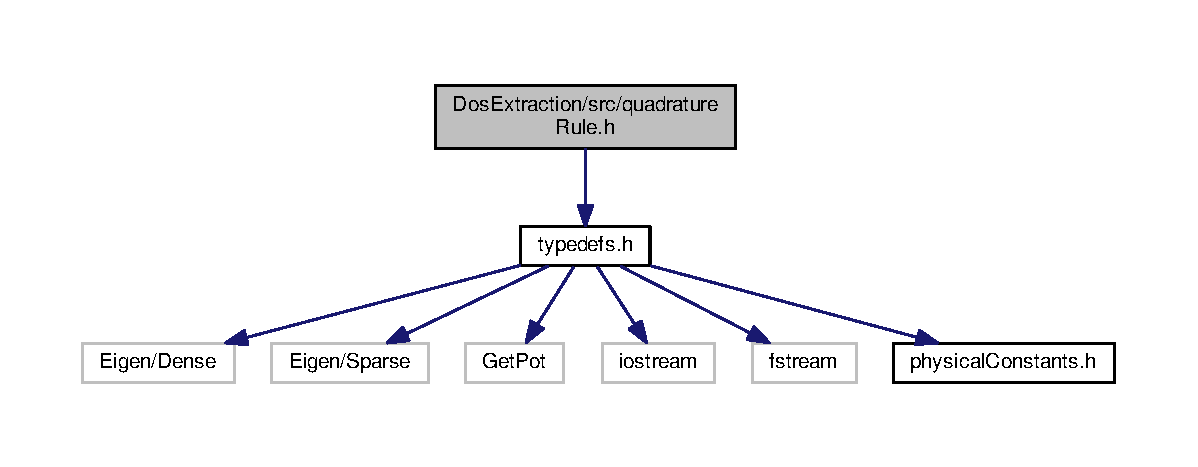
\includegraphics[width=350pt]{quadratureRule_8h__incl}
\end{center}
\end{figure}
This graph shows which files directly or indirectly include this file\-:\nopagebreak
\begin{figure}[H]
\begin{center}
\leavevmode
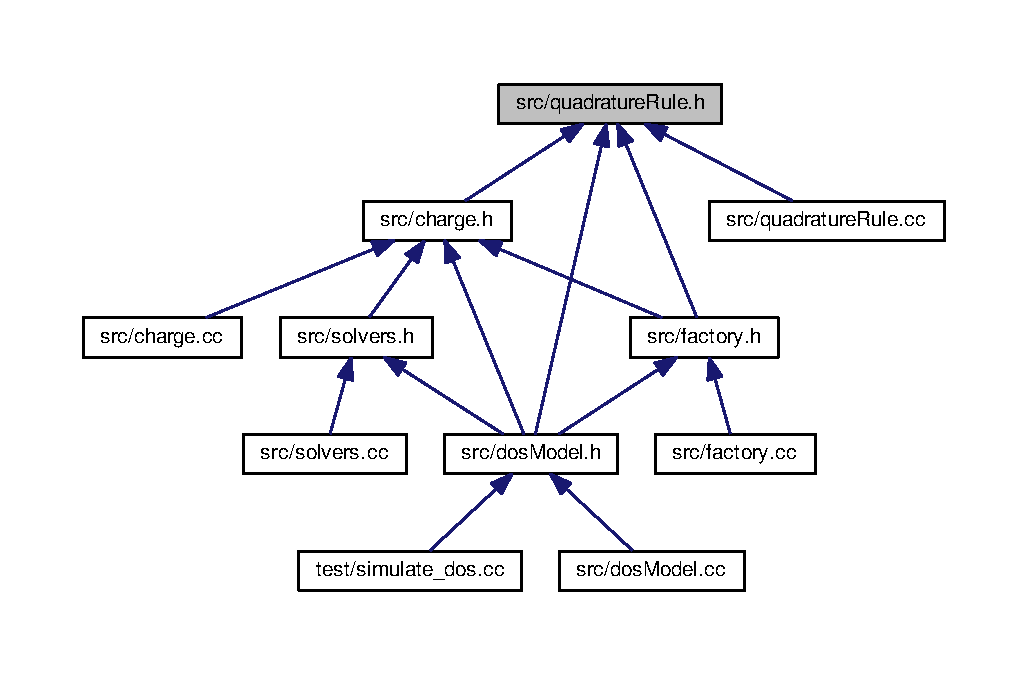
\includegraphics[width=350pt]{quadratureRule_8h__dep__incl}
\end{center}
\end{figure}
\subsection*{Classes}
\begin{DoxyCompactItemize}
\item 
class \hyperlink{classQuadratureRule}{Quadrature\-Rule}
\begin{DoxyCompactList}\small\item\em Abstract class providing a quadrature rule. \end{DoxyCompactList}\item 
class \hyperlink{classGaussHermiteRule}{Gauss\-Hermite\-Rule}
\begin{DoxyCompactList}\small\item\em Class derived from \hyperlink{classQuadratureRule}{Quadrature\-Rule} providing the Gauss-\/\-Hermite quadrature rule. \end{DoxyCompactList}\item 
class \hyperlink{classGaussLaguerreRule}{Gauss\-Laguerre\-Rule}
\begin{DoxyCompactList}\small\item\em Class derived from \hyperlink{classQuadratureRule}{Quadrature\-Rule} providing the Gauss-\/\-Laguerre quadrature rule. \end{DoxyCompactList}\end{DoxyCompactItemize}


\subsection{Detailed Description}
Quadrature rules. \begin{DoxyAuthor}{Author}
Pasquale Claudio Africa \href{mailto:pasquale.africa@gmail.com}{\tt pasquale.\-africa@gmail.\-com} 
\end{DoxyAuthor}
\begin{DoxyDate}{Date}
2014
\end{DoxyDate}
\begin{DoxyCopyright}{Copyright}
Copyright © 2014 Pasquale Claudio Africa. All rights reserved. 

This project is released under the G\-N\-U General Public License. 
\end{DoxyCopyright}


Definition in file \hyperlink{quadratureRule_8h_source}{quadrature\-Rule.\-h}.


\hypertarget{solvers_8h}{\section{Dos\-Extraction/src/solvers.h File Reference}
\label{solvers_8h}\index{Dos\-Extraction/src/solvers.\-h@{Dos\-Extraction/src/solvers.\-h}}
}


Generic solvers for P\-D\-Es.  


{\ttfamily \#include \char`\"{}charge.\-h\char`\"{}}\\*
{\ttfamily \#include \char`\"{}typedefs.\-h\char`\"{}}\\*
{\ttfamily \#include $<$utility$>$}\\*
{\ttfamily \#include $<$limits$>$}\\*
Include dependency graph for solvers.\-h\-:\nopagebreak
\begin{figure}[H]
\begin{center}
\leavevmode
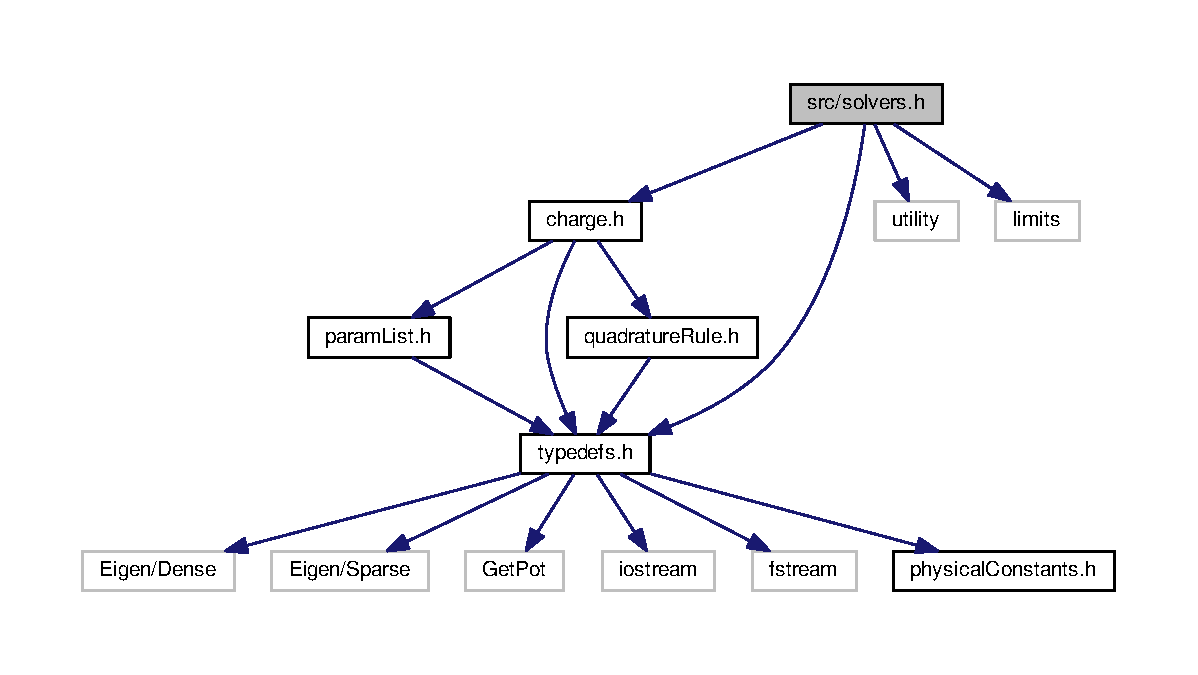
\includegraphics[width=350pt]{solvers_8h__incl}
\end{center}
\end{figure}
This graph shows which files directly or indirectly include this file\-:\nopagebreak
\begin{figure}[H]
\begin{center}
\leavevmode
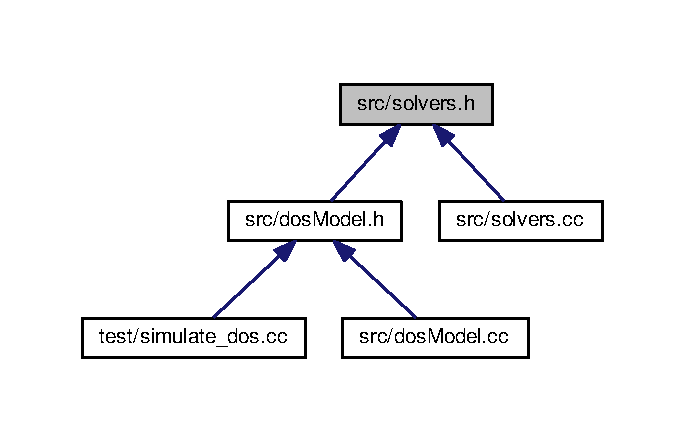
\includegraphics[width=329pt]{solvers_8h__dep__incl}
\end{center}
\end{figure}
\subsection*{Classes}
\begin{DoxyCompactItemize}
\item 
class \hyperlink{classPdeSolver1D}{Pde\-Solver1\-D}
\begin{DoxyCompactList}\small\item\em Abstract class providing methods to assemble matrices to solve one-\/dimensional P\-D\-Es. \end{DoxyCompactList}\item 
class \hyperlink{classBim1D}{Bim1\-D}
\begin{DoxyCompactList}\small\item\em Class derived from \hyperlink{classPdeSolver1D}{Pde\-Solver1\-D}, providing a finite volume Box Integration Method (B\-I\-M) solver. \end{DoxyCompactList}\item 
class \hyperlink{classNonLinearPoisson1D}{Non\-Linear\-Poisson1\-D}
\begin{DoxyCompactList}\small\item\em Provide a solver for a non-\/linear Poisson equation. \end{DoxyCompactList}\end{DoxyCompactItemize}


\subsection{Detailed Description}
Generic solvers for P\-D\-Es. \begin{DoxyAuthor}{Author}
Pasquale Claudio Africa \href{mailto:pasquale.africa@gmail.com}{\tt pasquale.\-africa@gmail.\-com} 
\end{DoxyAuthor}
\begin{DoxyDate}{Date}
2014
\end{DoxyDate}
\begin{DoxyCopyright}{Copyright}
Copyright © 2014 Pasquale Claudio Africa. All rights reserved. 

This project is released under the G\-N\-U General Public License. 
\end{DoxyCopyright}


Definition in file \hyperlink{solvers_8h_source}{solvers.\-h}.


\hypertarget{typedefs_8h}{\section{Dos\-Extraction/src/typedefs.h File Reference}
\label{typedefs_8h}\index{Dos\-Extraction/src/typedefs.\-h@{Dos\-Extraction/src/typedefs.\-h}}
}


Typedefs and utility functions.  


{\ttfamily \#include $<$Eigen/\-Dense$>$}\\*
{\ttfamily \#include $<$Eigen/\-Sparse$>$}\\*
{\ttfamily \#include \char`\"{}Get\-Pot\char`\"{}}\\*
{\ttfamily \#include $<$gnuplot-\/iostream.\-h$>$}\\*
{\ttfamily \#include $<$iostream$>$}\\*
{\ttfamily \#include $<$fstream$>$}\\*
{\ttfamily \#include \char`\"{}physical\-Constants.\-h\char`\"{}}\\*
Include dependency graph for typedefs.\-h\-:
\nopagebreak
\begin{figure}[H]
\begin{center}
\leavevmode
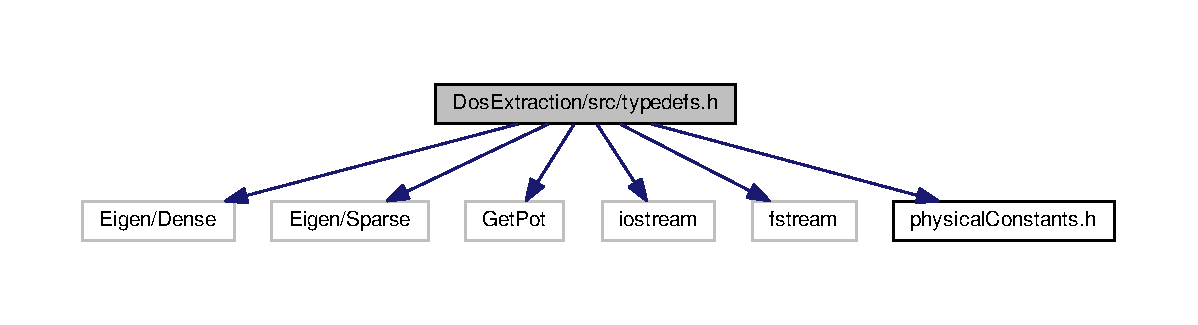
\includegraphics[width=350pt]{typedefs_8h__incl}
\end{center}
\end{figure}
This graph shows which files directly or indirectly include this file\-:\nopagebreak
\begin{figure}[H]
\begin{center}
\leavevmode
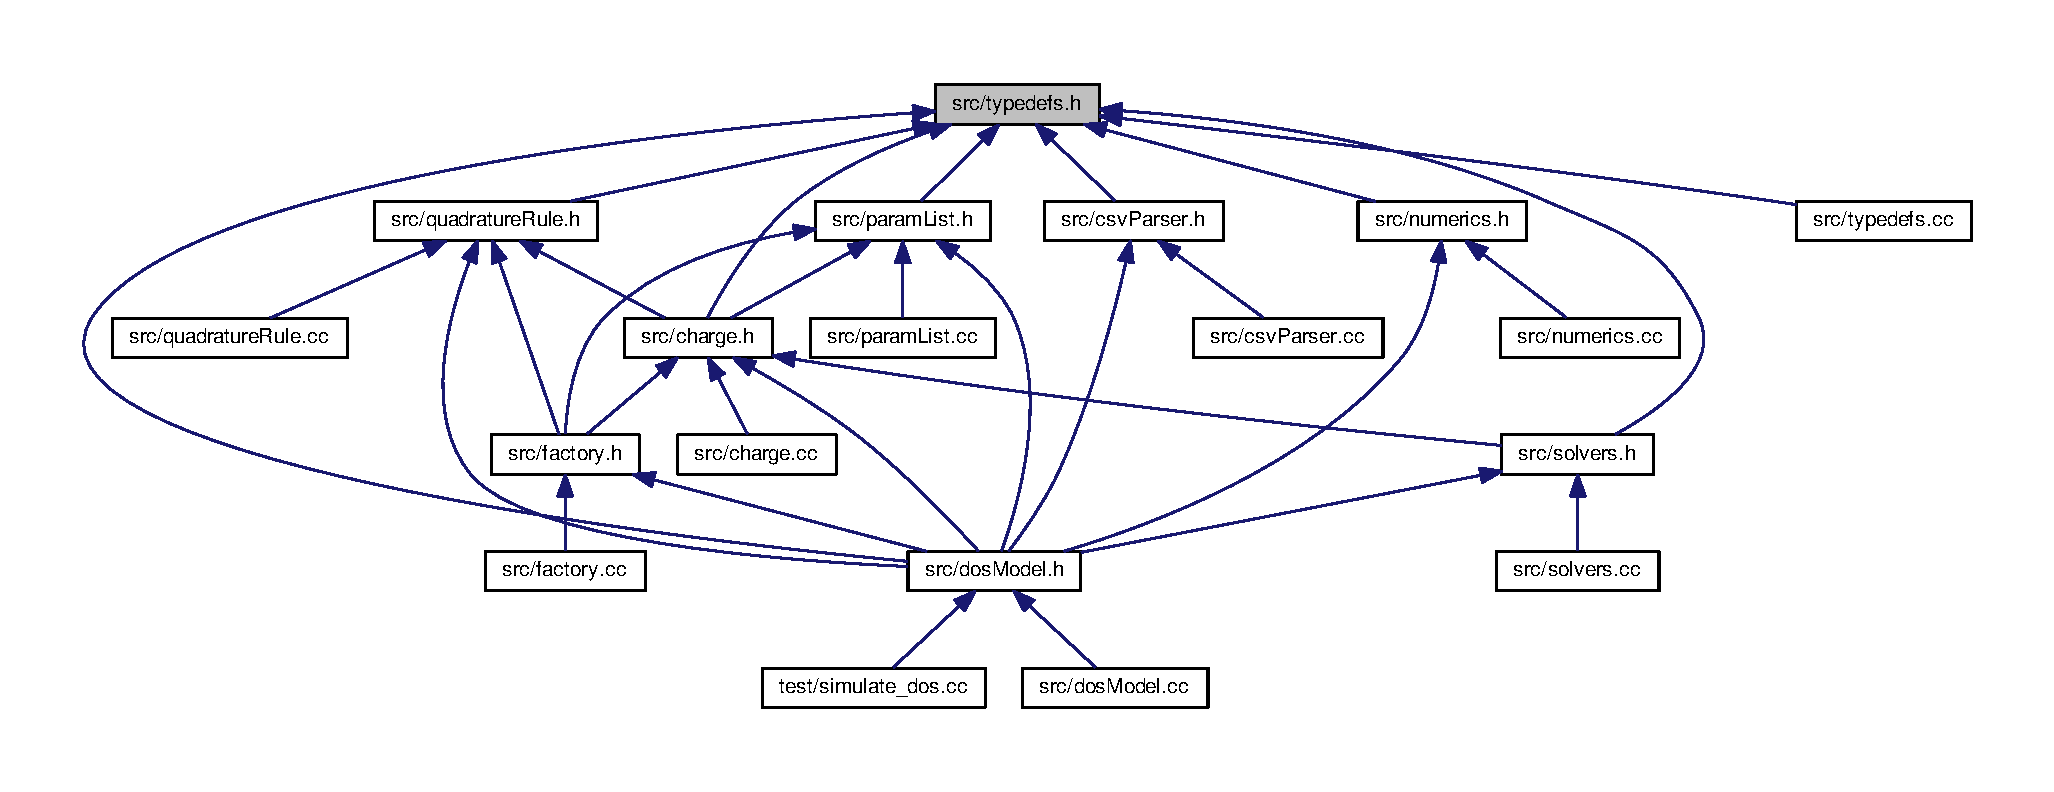
\includegraphics[width=350pt]{typedefs_8h__dep__incl}
\end{center}
\end{figure}
\subsection*{Namespaces}
\begin{DoxyCompactItemize}
\item 
\hyperlink{namespaceconstants}{constants}
\begin{DoxyCompactList}\small\item\em Numerical constants. \end{DoxyCompactList}\item 
\hyperlink{namespaceutility}{utility}
\begin{DoxyCompactList}\small\item\em Namespace for utilities and auxiliary functions. \end{DoxyCompactList}\end{DoxyCompactItemize}
\subsection*{Macros}
\begin{DoxyCompactItemize}
\item 
\hypertarget{typedefs_8h_a060b837c3b4486ee35317744156f3da2}{\#define \hyperlink{typedefs_8h_a060b837c3b4486ee35317744156f3da2}{Real}~double}\label{typedefs_8h_a060b837c3b4486ee35317744156f3da2}

\begin{DoxyCompactList}\small\item\em Pre-\/processor macro for real numbers. \end{DoxyCompactList}\item 
\hypertarget{typedefs_8h_a2c726f8f32697958e9d6c2afecda531d}{\#define \hyperlink{typedefs_8h_a2c726f8f32697958e9d6c2afecda531d}{Index}~ptrdiff\-\_\-t}\label{typedefs_8h_a2c726f8f32697958e9d6c2afecda531d}

\begin{DoxyCompactList}\small\item\em Pre-\/processor macro for indexing variables. \end{DoxyCompactList}\end{DoxyCompactItemize}
\subsection*{Typedefs}
\begin{DoxyCompactItemize}
\item 
\hypertarget{typedefs_8h_a81d507f5d0c665fb16966595c9520a55}{typedef Matrix$<$ \hyperlink{typedefs_8h_a060b837c3b4486ee35317744156f3da2}{Real}, Dynamic, \\*
Dynamic $>$ \hyperlink{typedefs_8h_a81d507f5d0c665fb16966595c9520a55}{Matrix\-Xr}}\label{typedefs_8h_a81d507f5d0c665fb16966595c9520a55}

\begin{DoxyCompactList}\small\item\em Typedef for dense real-\/valued dynamic-\/sized matrices. \end{DoxyCompactList}\item 
\hypertarget{typedefs_8h_aae6cee78ed9cd8f234ed8cb48682548a}{typedef Matrix$<$ \hyperlink{typedefs_8h_a060b837c3b4486ee35317744156f3da2}{Real}, Dynamic, 1 $>$ \hyperlink{typedefs_8h_aae6cee78ed9cd8f234ed8cb48682548a}{Vector\-Xr}}\label{typedefs_8h_aae6cee78ed9cd8f234ed8cb48682548a}

\begin{DoxyCompactList}\small\item\em Typedef for dense real-\/valued dynamic-\/sized column vectors. \end{DoxyCompactList}\item 
\hypertarget{typedefs_8h_aaf38a491cc6d8aeb1c1f53f380789bad}{typedef Matrix$<$ \hyperlink{typedefs_8h_a060b837c3b4486ee35317744156f3da2}{Real}, 1, Dynamic $>$ \hyperlink{typedefs_8h_aaf38a491cc6d8aeb1c1f53f380789bad}{Row\-Vector\-Xr}}\label{typedefs_8h_aaf38a491cc6d8aeb1c1f53f380789bad}

\begin{DoxyCompactList}\small\item\em Typedef for dense real-\/valued dynamic-\/sized row vectors. \end{DoxyCompactList}\item 
\hypertarget{typedefs_8h_a6d3b7db3fa8171d0e743df848524c269}{typedef Sparse\-Matrix$<$ \hyperlink{typedefs_8h_a060b837c3b4486ee35317744156f3da2}{Real} $>$ \hyperlink{typedefs_8h_a6d3b7db3fa8171d0e743df848524c269}{Sparse\-Xr}}\label{typedefs_8h_a6d3b7db3fa8171d0e743df848524c269}

\begin{DoxyCompactList}\small\item\em Typedef for sparse real-\/valued dynamic-\/sized matrices. \end{DoxyCompactList}\item 
{\footnotesize template$<$typename Scalar\-Type $>$ }\\using \hyperlink{typedefs_8h_ac264e7346c0c88c8a573518d1e8f8c3d}{Vector\-X} = Matrix$<$ Scalar\-Type, Dynamic, 1 $>$
\begin{DoxyCompactList}\small\item\em Template alias for \hyperlink{index_Eigen}{Eigen} vectors. \end{DoxyCompactList}\item 
{\footnotesize template$<$typename T $>$ }\\using \hyperlink{typedefs_8h_af38b14e4434227fa8e1b41e0d6632171}{Vector\-Xpair} = \hyperlink{typedefs_8h_ac264e7346c0c88c8a573518d1e8f8c3d}{Vector\-X}$<$ std\-::pair$<$ T, \hyperlink{typedefs_8h_a2c726f8f32697958e9d6c2afecda531d}{Index} $>$ $>$
\begin{DoxyCompactList}\small\item\em Template alias for an \hyperlink{index_Eigen}{Eigen} vector of pairs\-: ({\itshape Scalar\-Type}, {\itshape Index}). \end{DoxyCompactList}\end{DoxyCompactItemize}
\subsection*{Functions}
\begin{DoxyCompactItemize}
\item 
std\-::string \hyperlink{namespaceutility_ac713105bb0c74653e26a924689ecc8c3}{full\-\_\-path} (const std\-::string \&, const std\-::string \&)
\begin{DoxyCompactList}\small\item\em Auxiliary function to return the full path to a file. \end{DoxyCompactList}\item 
void \hyperlink{namespaceutility_afe82f121837a9a5c250e77d133632c15}{print\-\_\-block} (const char $\ast$, std\-::ostream \&=std\-::cout)
\begin{DoxyCompactList}\small\item\em Auxiliary function to print a string inside a block. \end{DoxyCompactList}\item 
void \hyperlink{namespaceutility_a226df4bf30ae6e01ba77b81f7f3e8993}{print\-\_\-done} (std\-::ostream \&=std\-::cout)
\begin{DoxyCompactList}\small\item\em Auxiliary function to print a \char`\"{}\-D\-O\-N\-E!\char`\"{} string. \end{DoxyCompactList}\end{DoxyCompactItemize}
\subsection*{Variables}
\begin{DoxyCompactItemize}
\item 
\hypertarget{namespaceconstants_a8d66156216c7101bc75f6f62a7449cf7}{const \hyperlink{typedefs_8h_a2c726f8f32697958e9d6c2afecda531d}{Index} \hyperlink{namespaceconstants_a8d66156216c7101bc75f6f62a7449cf7}{P\-A\-R\-A\-M\-S\-\_\-\-N\-O} = 26}\label{namespaceconstants_a8d66156216c7101bc75f6f62a7449cf7}

\begin{DoxyCompactList}\small\item\em Number of parameters required in input file. \end{DoxyCompactList}\item 
\hypertarget{namespaceconstants_af5340fb69690fffd134dcae882754638}{const \hyperlink{typedefs_8h_a060b837c3b4486ee35317744156f3da2}{Real} \hyperlink{namespaceconstants_af5340fb69690fffd134dcae882754638}{P\-I} = M\-\_\-\-P\-I}\label{namespaceconstants_af5340fb69690fffd134dcae882754638}

\begin{DoxyCompactList}\small\item\em $ \pi $. \end{DoxyCompactList}\item 
\hypertarget{namespaceconstants_a0ebb82a72cc0395d173fba22dff4d8c0}{const \hyperlink{typedefs_8h_a060b837c3b4486ee35317744156f3da2}{Real} \hyperlink{namespaceconstants_a0ebb82a72cc0395d173fba22dff4d8c0}{S\-Q\-R\-T\-\_\-\-P\-I} = std\-::sqrt(P\-I)}\label{namespaceconstants_a0ebb82a72cc0395d173fba22dff4d8c0}

\begin{DoxyCompactList}\small\item\em $ \sqrt{\pi} $. \end{DoxyCompactList}\item 
\hypertarget{namespaceconstants_a3b733bd721f65dc9124f4fb15af3da5c}{const \hyperlink{typedefs_8h_a060b837c3b4486ee35317744156f3da2}{Real} \hyperlink{namespaceconstants_a3b733bd721f65dc9124f4fb15af3da5c}{P\-I\-\_\-\-M4} = 0.\-7511255444649425}\label{namespaceconstants_a3b733bd721f65dc9124f4fb15af3da5c}

\begin{DoxyCompactList}\small\item\em $ \pi^{-\frac{1}{4}} $. \end{DoxyCompactList}\item 
\hypertarget{namespaceconstants_ab0c53d0b9c422d694073f97eb185d292}{const \hyperlink{typedefs_8h_a060b837c3b4486ee35317744156f3da2}{Real} \hyperlink{namespaceconstants_ab0c53d0b9c422d694073f97eb185d292}{S\-Q\-R\-T\-\_\-2} = std\-::sqrt(2)}\label{namespaceconstants_ab0c53d0b9c422d694073f97eb185d292}

\begin{DoxyCompactList}\small\item\em $ \sqrt{2} $. \end{DoxyCompactList}\end{DoxyCompactItemize}


\subsection{Detailed Description}
Typedefs and utility functions. \begin{DoxyAuthor}{Author}
Pasquale Claudio Africa \href{mailto:pasquale.africa@gmail.com}{\tt pasquale.\-africa@gmail.\-com} 
\end{DoxyAuthor}
\begin{DoxyDate}{Date}
2014
\end{DoxyDate}
This file is part of the \char`\"{}\-Dos\-Extraction\char`\"{} project.

\begin{DoxyCopyright}{Copyright}
Copyright © 2014 Pasquale Claudio Africa. All rights reserved. 

This project is released under the G\-N\-U General Public License. 
\end{DoxyCopyright}


Definition in file \hyperlink{typedefs_8h_source}{typedefs.\-h}.



\subsection{Typedef Documentation}
\hypertarget{typedefs_8h_ac264e7346c0c88c8a573518d1e8f8c3d}{\index{typedefs.\-h@{typedefs.\-h}!Vector\-X@{Vector\-X}}
\index{Vector\-X@{Vector\-X}!typedefs.h@{typedefs.\-h}}
\subsubsection[{Vector\-X}]{\setlength{\rightskip}{0pt plus 5cm}using {\bf Vector\-X} =  Matrix$<$Scalar\-Type, Dynamic, 1$>$}}\label{typedefs_8h_ac264e7346c0c88c8a573518d1e8f8c3d}


Template alias for \hyperlink{index_Eigen}{Eigen} vectors. 


\begin{DoxyTemplParams}{Template Parameters}
{\em Scalar\-Type} & \-: the scalar type. \\
\hline
\end{DoxyTemplParams}


Definition at line 48 of file typedefs.\-h.

\hypertarget{typedefs_8h_af38b14e4434227fa8e1b41e0d6632171}{\index{typedefs.\-h@{typedefs.\-h}!Vector\-Xpair@{Vector\-Xpair}}
\index{Vector\-Xpair@{Vector\-Xpair}!typedefs.h@{typedefs.\-h}}
\subsubsection[{Vector\-Xpair}]{\setlength{\rightskip}{0pt plus 5cm}using {\bf Vector\-Xpair} =  {\bf Vector\-X}$<$std\-::pair$<$T, {\bf Index}$>$ $>$}}\label{typedefs_8h_af38b14e4434227fa8e1b41e0d6632171}


Template alias for an \hyperlink{index_Eigen}{Eigen} vector of pairs\-: ({\itshape Scalar\-Type}, {\itshape Index}). 


\begin{DoxyTemplParams}{Template Parameters}
{\em Scalar\-Type} & \-: the scalar type. \\
\hline
\end{DoxyTemplParams}


Definition at line 55 of file typedefs.\-h.


%--- End generated contents ---

% Index
\newpage
\phantomsection
\addcontentsline{toc}{chapter}{Index}
\printindex

\end{document}
